\section{Využití iontových svazků v materiálovém výzkumu: Základní typy urychlovačů, Metody RBS, kanálování, PIXE, PIGE, ERDA a NRA}

\subsection{Základní typy urychlovačů}

- \underline{Definice:} Urychlovač je zařízení, které umožňuje zvýšení kinetické energie nabité (urychlované) částice, a to pomocí elektrické pole, které může být statické nebo proměnně a přitom je vede po stanovené trajektorii, a to pomocí megnetického pole, jež může být opět statické a nebo proměnné. Urychlovat lze pouze nabité částice, stejně tak jako je vést po určité dráze vlivem magnetického/elektromagnetického pole.

- Díky případnému konverznímu materiálu lze eventuelně převést nabité částice na jiný typ záření (neutrony, fotony).

\underline{Základní komponenty urychlovače:}

\begin{itemize}
    \item Zdroj nabitých částic
    \item Urychlovací trubice (elmg. pole)
    \begin{itemize}
        \item VN zdroj vytvářecí urychlovací napětí a magnety v urychlovačí (dipóly = zakřivení dráhy pohybu částic, kvadrupóly = fokusace svazku).
    \end{itemize}
    \item Systém dodávky ELMG. polí
    \item Extrakce urychlených částic z urychlovače a soustředění na terčík
    \item bombardovaný terčík a detektor/y pro popis parametrů urychleného svazku
    \item Diagnostika svazku (sledování energie, intenzity, polohy)
    \item Systém napájení
    \item řídicí systém
    \item vakuový systém

\end{itemize}

\underline{Rozdělení:}

\begin{itemize}
    \item Dle trajektorie - Dle trajektorie rozdělujeme urychlovače na lineární(elektrostatické=konst. urychlovací napětí a rezonanční=časově proměnlivé urychlovací napětí) a cyklické(mikrotron, betatron, cyklotron, synchrotron, synchocyklotron, izochronní cyklotron).

    \item Dle způsobu urychlení - Dle způsobu urychlení rozdělujeme Elektrostatické a Rezonanční, což je například pro lineární urychlovače velmi efektivní a jsme schopni získat jednotky až desítky MeV na jednotkách metrů (1m je cca jednotky až destíky MeV)

    \item Dle režimu práce - Nepřetržité (časově neměnný svazek) a Impulzní (uvolňování částic po částech/balících).
\end{itemize}

\underline{Princip urychlení a zakřivení}:

Velmi to záleží jestli mám cyklický a nebo lineární a pak podle typu napětí a mag. pole.

\begin{itemize}
    \item Lineární elektrostatický -> v tomto případě mám rovnou trubici, kde mám dáno urychlovací napětí konstatní a částice je na dáne dráze urychlena tak moc, jak je dáno napětí. Magnetické pole pak zde slouží v podobě dipólů nebo kvadrupólů, a to pro korekci svazku, aby se nevychyloval a pro jeho fokusaci. K tomu se pak typicky ale využívá tzv. elektrostatický fokusační systém, který je tvořen 4 elektrodami, jež jsou vždy 2 a 2 naproti sobě se stejným napětím a způsobují, že částice je "odrážena" doprostřed.
    \item Lineární rezonanční -> Přímočará dráha pohybum proměnlivý proud (napětí se cyklicky mění a jednotlivé elektrody mění náboj, aby buď odpuzovaly či přitahovaly), zvětšující se délka urychlovacích segmentů s délkou (částice se hýbe velmi rychle, tak to musí mít nějaký efekt a aby ji to vůbec stihlo urychlit, tak jsou delší a delší). Hodně se to využívá v medicíně, protože na krátké vzdálenosti naberou částice vysokou energii a poté se využívá např. převod elektronu na RTG či $\gamma$. V klidu se dá urychlit na 10-15 MeV/m

    \item Cyklický (konst. napětí i magnetické pole) -> V tomto případě přiletí částice a urychlovacím napětím jí roste energie a magnetickým polem je zakřivena její dráha pohybu, která se s jeho konstatností zvětšuje v poloměru. Celý urychlovač je navržen tak, že při správné energii dosáhne částice maximálního poloměru dráhy pohybu a vyletí ústím ven.

    \item Cyklický (konst. napětí) -> Stejné jako výše, avšak pomocí proměnlivého magnetického pole mohu částici udržovat na stejném poloměru zakřivení.

    \item Cyklický (obojí proměnlivé) -> Mám tam například místa, kde když částice projde, tak ji to urychlý a stejně jako u lineárního dochází k periodickému přepólování, aby částice byla odpuzována/přitahována ve správný moment. Proměnlivým magnetickým polem je pak držena na stejném poloměru.
\end{itemize}

\underline{Využití:} Materiálový výzkum, částicová fyzika, Produkce radionuklidů (do medicíny či materiálový výzkum), Produkce neutronů (studium radiačního poškození, difrakce neutronů, neutronová fyzika, produkce fotonů (materiálový výzkum-XFEL a medicína).


\subsection{Metoda RBS}
- Rutherford Backscatterring Spectroscopy
- Využití pružného rozptylu nalétávajících iontů z monoenergetického svazku (E=1-3 MeV) s atomy či jejich elektrony v terčíku.
\begin{itemize}
    \item Pružný rozptyl = bez ztráty energie na srážku
    \item Měření počtu a energii odražených iontů dopadajícího svazku, což nám dává info o materiálu terčíku.
    \item typické hloubky, kde je RBS schopno identifikovat a lokalizovat různé prvky v matrici jsou desítky až stovky nm.
\end{itemize}


\underline{výhody}:
\begin{itemize}
\item vysoká citlivost na těžké prvky v lehké matrici
\item jednoduché umístění vzorku na vzduchu
\item kvalitativní přesnost < 1 \%
\item hloubkové rozlišení < 5 nm se Si(Li) detektorem
\item kanálování
\item Vysoká přesnost na těžké prvky v lehké matrici
\item Schopnost velmi dobře rozlišit dva lehké prvky mezi sebou navzájem (dva lehké prvky s malým rozdílem hmotnosti), a to např. 18-O a 19-F, 13-C a 14-N
\end{itemize}

\underline{nevýhody}:
\begin{itemize}
\item necitlivé na lehké prvky v těžké matrici
\item implantování iontů do analyzovaného materiálu
\item potřebný urychlovač
\item Problém rozlišit dva těžké prvky o podobné hmotnosti (208-Pb a 197-Au), avšak rozlišovací schopnost lze zlepšit zvýšením hmotnosti dopadající částice ($M_1$)=citlivost při dopadu alfa částice je lepší v porovnání s protony.
\end{itemize}

\begin{figure}[ht!]
	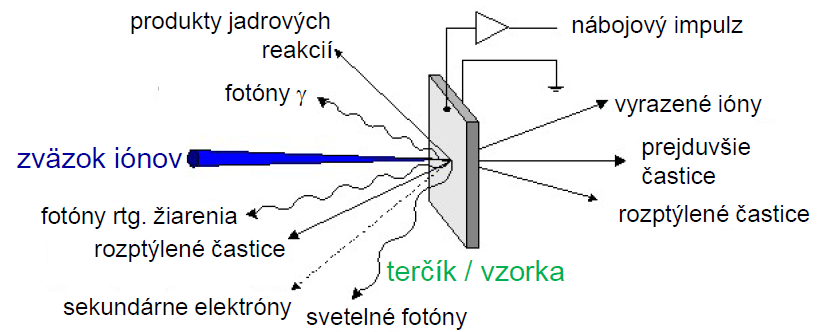
\includegraphics[width=10cm]{iont-svazky.png}
	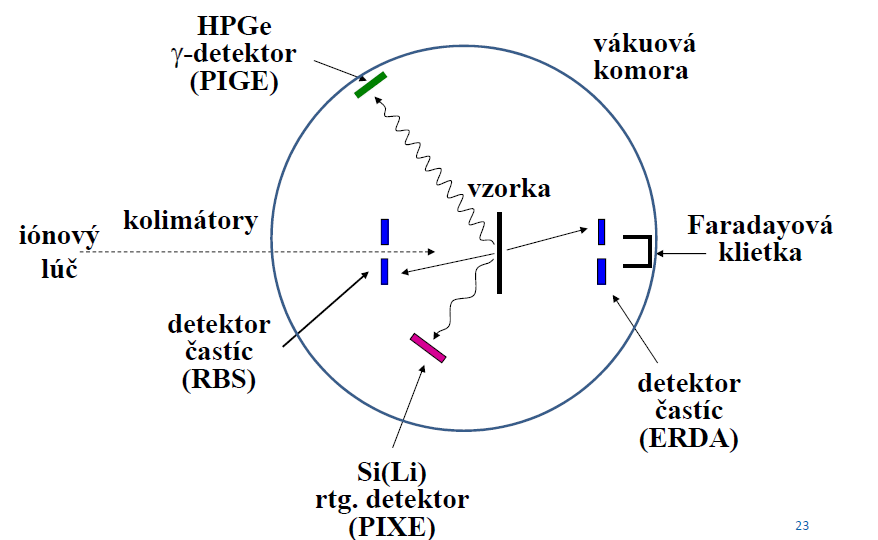
\includegraphics[width=7cm]{iont-svazky-exp.png}
\end{figure}

V zásadě existují dva procesy, resp. interakce urychlených iontů s danou látkou:\\

1) \underline{Interakce s jádrem (Elastický Coulombův rozptyl) }
\begin{itemize}
    \item Víme počáteční energii $E_0$, víme jeho hmotnost $M_1$ a měříme jeho energii $E_1$ po jeho zpětném rozptylu.
    \item Využijeme $E_1$ = K * $E_0$, kde K je kinematický faktor a je funkcí hmotností obou interagujících částic a úhlu odrazu zaznamenáného odraženého iontu
    \item Neznámou tedy představuje pouze hmotnost $M_2$, kterou jsme schopni z toho dopočítat a určit o jaké jádro se jedná.
\end{itemize}

2) \underline{Interakce s elektrony (elektronový rozptyl)}
\begin{itemize}
    \item Lokalizace a určení atomu ($M_2$) jakožto funkce hloubky, resp. v závislosti na tom v jaké hloubce dojde k rozptylu.
    \item množství úbytku energie záleží na brzdném účinku látky, tedy na hustotě elektronů v látce a vzdálenosti, kterou nabitý iont urazí při průchodu látkou.
    \item Prvky, které se v materiálu objevují pouze v určité hloubce mají na naměřeném spektru svůj pík posunuty, ale jsou posunuty o jistou míru/energii, která představuje vzdálenost, kterou musel iont projít materiálem, aby se k nim dostal.
    \item Ke stanovení je nutné mít naměřenou energii iontu po odrazu na povrchu a pak následně v dané hloubce. Čím hlouběji iont musel jít, tím více ztratí energie
    \item Správnost určení rozdílu energií při odrazu na povrchu a v hloubce ($\Delta E$) závisí na = energetické rozlišení detektoru, energetický rozptyl urychleného svazku dopadajících iontů a také energetický rozptyl směrem k a od terčíku, příprava povrchu terčíku. Na závěr samozřejmě závisí na materiálu, který je měřen.
\end{itemize}

\underline{Měřené spektrum podle tloušťky měřeného vzorku materiálu}
\begin{itemize}
    \item Ultra tenká vrstva (několik atomárních vrstev)

    \begin{figure}[ht!]
        \centering
        \includegraphics[width=0.5\linewidth]{ultra tenká vrstva - RBS.png}
        \caption{ultra tenká vrstva - RBS}
    \end{figure}

    \item Tenká vrstva (několik stovek až tisíců atomárních vrstev)

    \begin{figure}[ht!]
        \centering
        \includegraphics[width=0.5\linewidth]{Tenká vrstva - RBS.png}
        \caption{Tenká vrstva - RBS}
    \end{figure}

    \item Hrubá vrstva = toto už jsou mm, v zásadě bulk/objem.

    \begin{figure}[ht!]
        \centering
        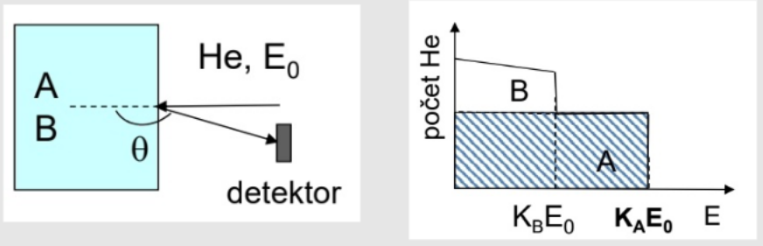
\includegraphics[width=0.5\linewidth]{Bulk - RBS.png}
        \caption{Bulk - RBS}
    \end{figure}

    \item Pokrytí povrchu = bulk materiál, který má na povrchu naneseny různé tloušťky jiného materiálu/materiálů. Zde rozdělujeme 2 varianty (lehký bulk a těžké pokrytí a naopak)

    \begin{figure}[ht!]
        \centering
        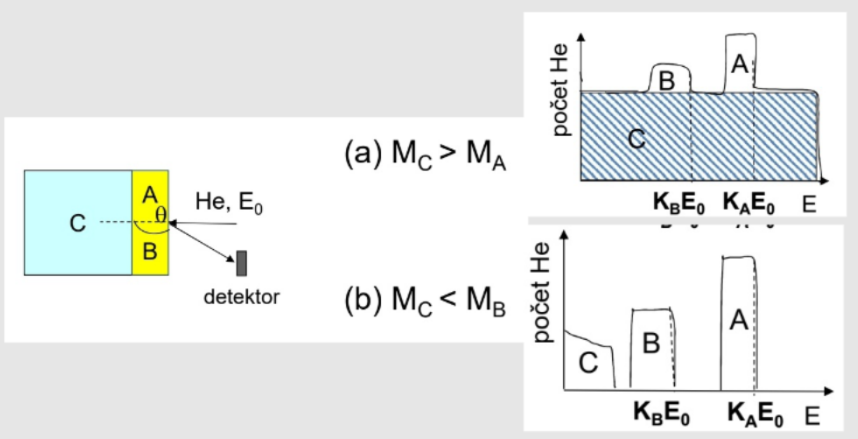
\includegraphics[width=0.5\linewidth]{pokrytí - RBS.png}
        \caption{pokrytí - RBS}
    \end{figure}
\end{itemize}

\noindent- kvalitativní analýza 
\begin{figure}[ht!]
	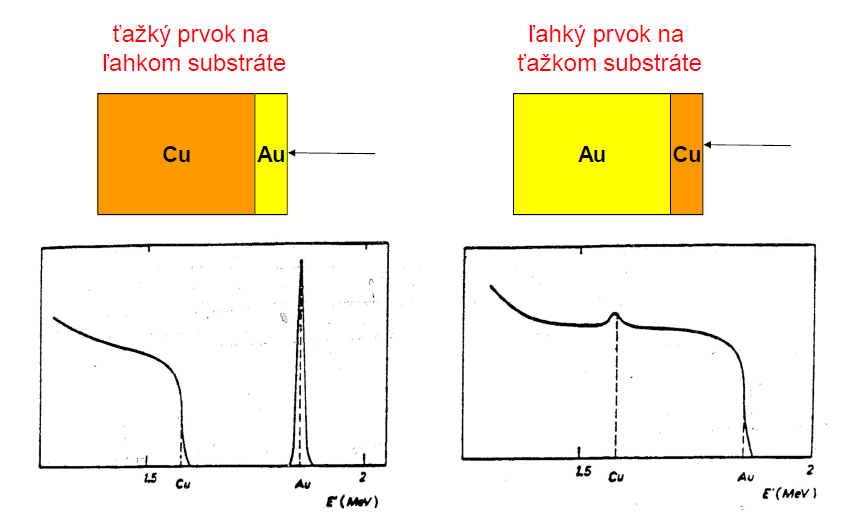
\includegraphics[width=9cm]{rbs-analyza.png}
	%	\includegraphics[width=7cm]{rbs2.png}
	%	\includegraphics[width=7cm]{rbs3.png}
\end{figure}


Výstupem při měření dostáváme z detektoru impulsy, jejichž výška je úměrná energii zpětně odraženého iontu. Z výšky čar výsledného spektra lze stanovit stechiometrické složení vzorku.\\

\underline{Využití:}

-Detektory částic nastavené na RBS jsou často součásti většího celku jehož součásti jsou i detektory na PIGE, PIXE, ERDA a celé to bývá vaukováno, aby nedocházelo k parazitní interakci s částicemi atmosféry (nahoře je ovšem psáno, že RBS jde dělat i na vzduchu, což jde, ale je lepší tam tu parazitní interakci nemít).

-Umění, archeologie (sochy, obrazy, předměty - například rozdíl mezi zlatem a pozlacením), Materiálový výzkum a Geologie.

\subsection{Kanálování}

- Kanálování je speciální mód RBS techniky. Vyžadováno je, aby orientace urychlených iontů byla ve správné poloze vůči krystalografické mříži, a to konkrétně podél hlavní krystalografické osy krystalu.

- V čistém a ideálním krystalu by měl iont jakoby "projít rovně skrz  a mezi jednotlivými rovinami", avšak v případě přítomnosti poruch či příměsí jsme schopni detekovat jejich polohu v krystalu, jelikož pak dochází k poklesu intenzity detekovaného záření (stínení Coulombovského rozptylu).

\begin{figure}[ht!]
	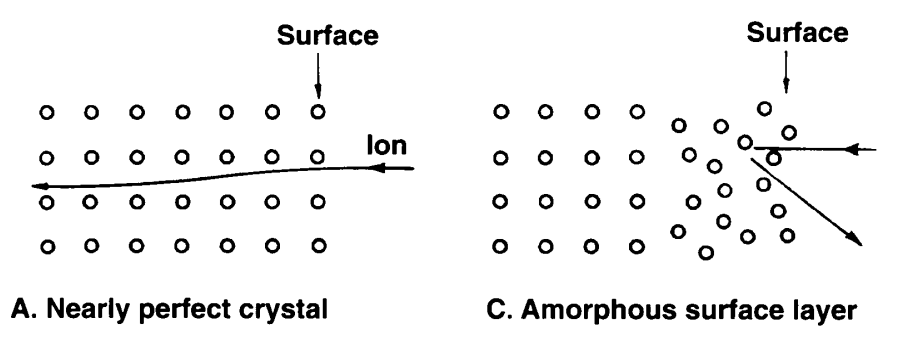
\includegraphics[width=10cm]{rbs-kanalovani.png}
	%	\includegraphics[width=7cm]{rbs2.png}
	%	\includegraphics[width=7cm]{rbs3.png}
\end{figure}

\subsection{PIXE}
PIXE je tzv. Particle Induced X-Ray Emission a jedná se nedestruktivní o metodu, která využívá detekce charakteristického RTG záření.

\underline{Výhody:}
\begin{itemize}
    \item Nedestruktivní technika schopna měřit tuhé látky, tekutiny i aerosoly
    \item Vysoká citlivost a rychlost měření
    \item Dobrá rozlišovací schopnost = multiprvková analýza (Z>13 = Al)
\end{itemize}

\underline{Nevýhody:}
\begin{itemize}
    \item Nelze analyzovat organické vzorky
    \item Omezená hloubková informace
    \item Potřeba urychlovače
\end{itemize}

\underline{Princip:}

- Excitací atomu iontovým svazkem (vyražení elektronu a jeho zabrání elektronem z vyšší energetické hladiny) a produkce charakteristického RTG záření, jehož detekči lze identifikovat původce a identifikovat tak prvek (v zásadě stejné jako u RFA, akorát tady se využívají ionty a ne fotony z radionuklidu nebo rentgenky).

- Stejně jako u RFA, tak i zde je Augerův elektron konkurenční jev a dohromady dávají jedničku. Takže existuje klasicky pravděpodobnost, že k vyzáření RTG dojde a ta je dána účinným průřezem pro ionizaci a fluorescenčním výtěžkem.

- Stejně jako u RFA, tak se projevují matricové jevy, které mi ovlivňují měření, tedy to co naměřím a to co realně je ve zkoumaném materiálu.

- Stejně jako u RFA, tak plocha pod čarou je rovna koncentraci prvku

- K detekci charakteristického RTG záření se využívá HPGe, Si(Li)

\begin{figure}[ht!]
	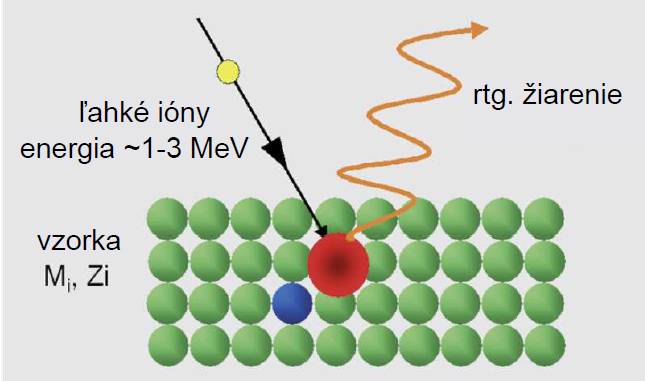
\includegraphics[width=8cm]{pixe.png}
	%	\includegraphics[width=7cm]{rbs2.png}
	%	\includegraphics[width=7cm]{rbs3.png}
\end{figure}

\underline{Aplikace a využití:}
\begin{itemize}
    \item Materiálový výzkum
    \item Geologie
    \item Umění, architektura
    \item Monitoring znečištění atmosfŕy
\end{itemize}

\underline{Speciální případy:}
\begin{itemize}
    \item Mikrosvazek = distribuce prvků ve vzorku (analýza hrubých vrstve s vysokým rozlišením) -> stopová množství, malé oblasti s vysokým rozlišením.
    \item Externí svazek = Analýza velkých a komplexních předmětů svazkem z urychlovače, který je vyveden ven do atmosféry na zkoumaný objekt (proto externí svazek)-> Louvre, artefakty, obrazy.
\end{itemize}


\subsection{PIGE}
-PIGE = Particle Induced Gamma Emission

-Jedná se o nedestruktivní metodu pro stanovení prvkového složení na základě interakce urychlených protonů, popř. d, $\alpha$ a málokdy těžkých iontů s jádrem atomu za vzniku gama záření, které poté detekujeme. Toto záření tak je pak v některých případech doprovázeno ještě další reakcí, resp. vznikem další částice/záření

-Nejčastěji se opět měří ve vakuové komoře a nejvíce se využívají urychlené protony

\begin{itemize}
    \item Rezonanční záchyt (p, $\gamma$) - mohu využít rezonancí prvků, které jsou ve zkoumaném materiálu a pak detekuji jen gamu. To ale vyžaduje, že vím co tam je, resp. vím co v tom hledám, abych danou rezonanci mohl využít.

    \item nepružný záchyt (p, $p^| \gamma$)

    \item Srážky s přeuspořádáním (p, n$\gamma$), (p, $\alpha\gamma$), (p,n)
\end{itemize}

\subsection{ERDA}

-ERDA = Elastic Recoil Detection Analysis


-Jedná se o metodu využívající pružný rozptyl lehkých jader po dopadu těžkých iontů

-Slouží pro detekci lehkých prvků v těžké matrici (dokáže detekovat vodík v tuhých látkách)

\underline{Výhody:}
\begin{itemize}
\item Dobrá citlivost na lehké prvky
    \item Dá se kombinovat s RBS
    \item Menší poškození vyšetřovaného materiálu
    \item Idektifikace 1-H a 2-H hloubkových profilů (pomocí alfa).
\end{itemize}

\underline{Nevýhody:}
\begin{itemize}
    \item Menší hloubkové rozlišení a hloubka analýzy (způsobeno hmotností, resp. velikosti těžších iontů) je kvůli rozptylu dopadajících iontů asi několik stovek nm
    \item Vzorek musí být spešl připraven + omezená geometrie ozařování a detekce.
\end{itemize}

\underline{Princip:}
- Pružný rozptyl dopadajícíh vysokoenergetických a těžkých iontů (MeV) a ven jdou odražené ionty a vyražené atomy z materiálu.

- Umožňuje profilování lehkých jader

- S využitím standardů umožňuje i kvantitativní analýzu

\begin{figure}[ht!]
	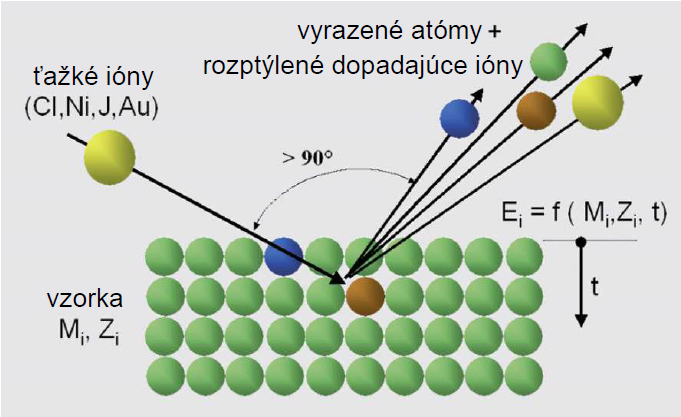
\includegraphics[width=8cm]{erda.png}
	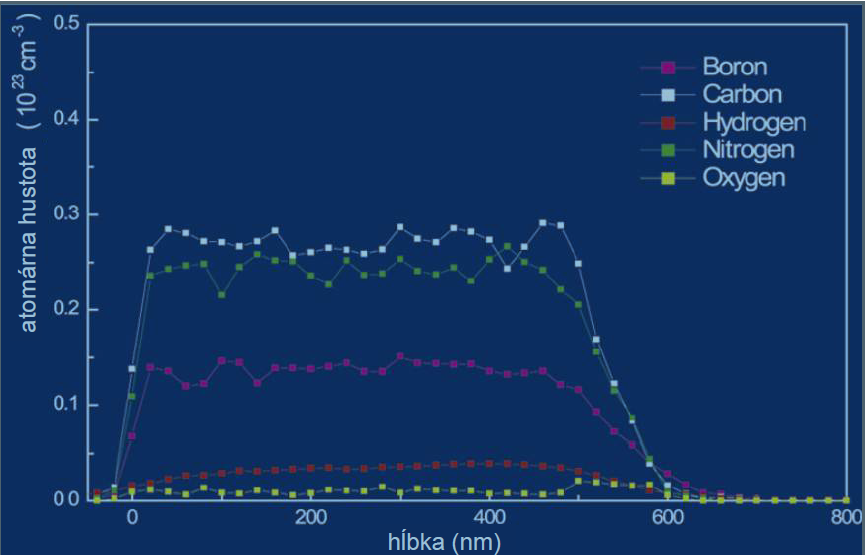
\includegraphics[width=7cm]{erda-spektrum.png}
	%	\includegraphics[width=7cm]{rbs3.png}
\end{figure}

\underline{Módy provozu:}

\begin{itemize}
    \item Transmisní: Velmi tenké vzorky

    \begin{figure}[ht!]
        \centering
        \includegraphics[width=0.38\linewidth]{transmisní ERDA.png}
        \caption{transmisní ERDA}
    \end{figure}

    \item Odraz pod malými úhly = nejčastější metoda

    \begin{figure}[ht!]
        \centering
        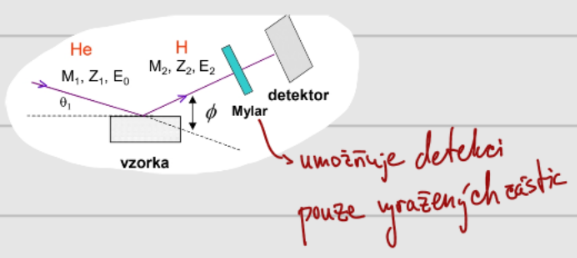
\includegraphics[width=0.5\linewidth]{odrazová ERDA.png}
        \caption{odrazová ERDA}
    \end{figure}
\end{itemize}

- V obou geometriích platí, že $E_2 = K * E_0$, kde faktor $K$ závisí na hmotnostech bombradující a vyražené částice a dále na úhlu rozptylum takže pak jen určíme zase hmotnost $M_2$.



\subsection{NRA}
- NRA = Nuclear Reaction Analysis

-Jedná se o metodu pro detekci lehkých prvků (Z<18), jež je izotopicky citlivá a umožňuje identifikaci a lokalizaci stopových prvků. Jedná se o nedestruktivní metodu s analytickou hloubkou několik stovek nm, ovšem jedná se vždy o exotermickou nebo endotermickou reakci a tudíž energetická bilance je vždy nenulová.

- Jedná se o nepružný proces, a proto se částice na začátku nerovnají produktům reakce.

\underline{Princip:}

-Jaderná reakce mezi dopadajícím iontem a prvkami v terčíku. Následně dochází k detekci produktů reakce ($\gamma$ nebo částice).

\begin{figure}[ht!]
	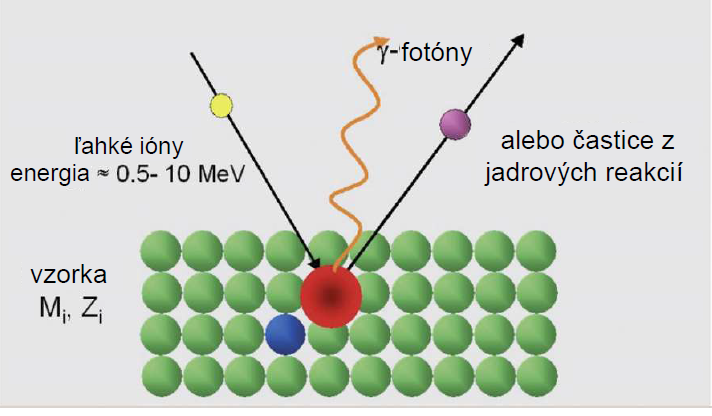
\includegraphics[width=8cm]{nra.png}
	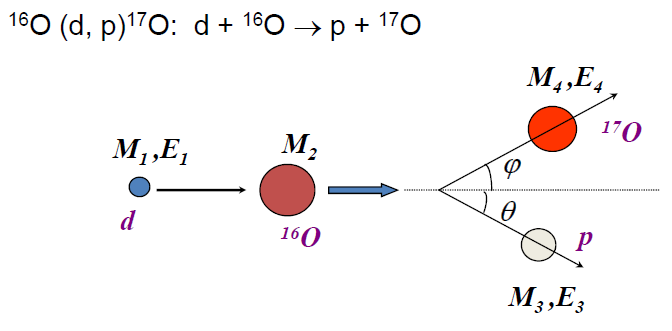
\includegraphics[width=7cm]{nra2.png}
	%	\includegraphics[width=7cm]{rbs3.png}
\end{figure}

- Detekuji produkty reakce (částice nebo $\gamma$)( pomocí Si detektoru nebo $\gamma$ fotony detekuju pomocí Ge či NaI(Tl) detektorů)a změřím si energii $E_3$ pro dané $M_1$, $E_1$ a $\theta$ a tím identifikuji $M_2$.

- Poté si naměřím spektrum $E_3$, které mi podá informaci o hloubkovém rozložení $M_2$ a tím ho lokalizuji v materiálu.
\\

\underline{Pozn.:} Reakce může probíhat dvojím způsobem, a to sice přes složené jádro (všechny nukleony jsou využity) a nebo jakožto tzv. přímá reakce, kde jen některé nukleony jsou použité (někdy nazýváno trhací reakce).
\\

- Pravděpodobnost reakce je klasicky dána příslušným účinným průřezem.
\\

- K detekci příslušných jader v hloubce nebo na povrchu se dají využít rezonance, kdy pokud se energie bombardující částice rovná energii rezonance, tak k interakci dojde na povrchu. Pokud je ovšem energie částice vyšší než energie rezonance, tak k interakci dojde v hloubce pod povrchem (cestou do materiálu se energie sníží a až se vyrovná tak interaguje).

- Příkladem je analýza vodíku pomocí 15-N za vzniku 12-C + 4-He a $\gamma$. Rezonance je při 6,385 MeV a s hloubkou dochází k posuvu rezonance, a proto se vyuźívájí energie vyšší než rezonance až napŕ. do 15 MeV.
\\

\underline{Využití:} Farmacie, archeologie, Geovědy, umění
\\
s
\underline{Srovnání RBS a NRA:}

\begin{itemize}
    \item RBS je pro detekci těžkých prvků v lehké matrici, zatímco NRA je pro detekci lehkých prvků.
    \item RBS využívá elastický rozptyl dopadajících částic (typicky $\alpha$ = 2 MeV), zatímco NRA vyuźívá nepružný roztpyl mezi dopadající částicí a částicí v terčíku (detekce produktů reakce)
    \item RBS má energetickou bilanci nulovou a NRA nemá
    \item u RBS jsou jádra terčíku i dopadající částice v základním stavu, zatímco u NRA jsou produkty reakce odlišné od původních, které do reakce vstupují.
\end{itemize}

\newpage
\section{Využití jaderně fyzikálních metod v materiálovém výzkumu: Mossbauerova spektrometrie, elektron-pozitronová anihilační spektrometrie, neutronová aktivační analýza}


\subsection{Mossbauerova spektrometrie}
- objevena německým fyzikem Rudolfem Mossbauerem 1958

- založeno na rezonanční fluorescenci $\gamma$ záření

- obvykle používané prvky: \iso{57}{Fe}, \iso{119}{Sn}, \iso{121}{Sb}, \iso{129}{I}

- široká škála aplikací při studiu chemických vazeb, anorganické chemii pevných látek, atd. Hlavní množství článků a studií je ale zaměřeno na železo.

-Jedná se o metodu izotopicky citlivou (bezodrazová jaderná rezonanční absorpce/fluorescence gama záření).

\subsubsection{Princip}

- Mossbauerův jev = bezodrazová jaderná rezonanční absorpce gamma záření

\begin{itemize}
    \item založeno na emisi a absorpci $\gamma$ záření emitovaného jádrem bez zpětného rázu

    \item atomy ve zdroji emitující $\gamma$ záření musí být stejné, jako v atomy ve vzorku

    \item vlastně je to tak, že jádra ve vzorku jsou excitovaná gammou, která je emitovaná při stejné deexcitaci ve zdroji


    \item Zde zdroje fotnů jsou generovány fotony o dané energii a pokud je tato energie veeeelmi přesná jako je energie mezi vzbuzeným a základním stavem atomu či jádra ve zkoumaném materiálu, tak dojde k tzv. rezonanční absorpci.

    \item Poté dochází opět k přechodu zkoumaného jádra do základního stavu emisí fotonu o té samé energii, co to původně vyvolala

    \item Celé co chceme je dosáhnout překrycu emisní a absoprpční čáry, což je velmi složité neboť je šířka píku (energie) velmi malá a komplikuje to celé jev tzv. zpětného rázu.
\end{itemize}

\subsubsection{Zpětný ráz}
\begin{itemize}

\item při emisi vysokoenergetické částice z jádra funguje zpětný odraz, část hybnosti je předaná emitujícímu jádru (analogicky u zbraně - taky mě to hodí trochu dozadu)

\item energie gamma záření má proto o trošku nižší energii než je energie rezonance, a to o energii tohoto zpětného rázu.

\item pro energii zpětného rázu platí: $E_{R} = \dfrac{E_{\gamma}}{2 M c^2}$, kde $M$ je hmotnost emitujícího jádra a $E_{\gamma}$ je energie emitovaného fotonu

\item s narůstající hmotností $M$ klesá energie zpětného odrazu, a proto platí, že jeli energie emitovaného gama záření malá oproti hmotnosti jádra, jež jej emituje, pak se energie zpětného rázu pohltí a s jádrem to nehne. V opačném případě je třeba tuto energii nějak zohlednit a ideálně ji kompenzovat.

\item v případě nevázaného jádra je posun energie značný a není možné Mossbauerův jev pozorovat. Neboli nedojde k překryvu emisní a absorpční čáry.

- Příkladem je známé železo 57-Fe u něhož je šířka čáry 4,6 neV a energie zpětného rázu je 2meV. To znamená, že emitované gama o velikosti 14.4 keV, které na něj letí s cílem ho excitovat, tak mi je k ničemu, protože energie fotonu je nižší o ty 2 meV a tudíž nedosáhnu překryvu emisní a absorpční čáry, která je ultra tenounká. Nutno dále zmínit, že o energii zpětného rázu se mi navíc posouvá nejen emisní čára, ale i absorpční čára, neboť to má vliv i na jádro, jež energii přijíma. Souhrně řečeno: U volného jádra (plynné či kapalné médium) dochází při emisi k zpětnému rázu, o který se sníží energie emitovaného fotonu a pak nevystačuje energie na excitaci cílového jádra.

\item Zvýšení hmotnosti jádra, aby byla energie zpětného rázu pohlcena/kompenzována lze dosáhnout uvázáním jádra do krystalické mřížky -> zpětný ráz je daleko menší, do hmotnosti se taky připočítávají okolní vázané atomy, neboli mřížka tlumí odraz.
\end{itemize}


\underline{Jak to funguje:}

\begin{itemize}
    \item Mám zdroj, který emituje přesně energii, kterou chci pro excitaci atomu/jádra v mém vzorku (pro tyto účely uvažujme 57-Fe

    \item Ve vzorku mám atomy/jádra 57-Fe, které toto záření absorbují, jsou excitována a poté při deexcitaci emitují gama záření o té samé energii, která je excitovala z mého zdroje (jak bylo řečeno výše, tak zdrojem je to samé jádro, které chci ve vzorku excitovat. Toto jádro, které já beru jako zdroj tak excituju nějakým externím RN zdrojem například).

    \item Emitované záření ze vzorku je pak emitované do celého prostorového úhlu.
\end{itemize}

\begin{figure}[ht!]
    \centering
    \includegraphics[width=\linewidth]{Mossbauer excitace jádra.png}
    \caption{Mossbauer excitace jádra}
\end{figure}




%\subsubsection{Dopplerův efekt}
%- způsobený tepelným pohybem jader
%
%- dochází k rozšiřování rezonancí, platí $$E_{\gamma} = E_0 - E_R + E_D,$$ kde $E_D = k\cdot v \cdot \cos(\beta/c)$
%
%- rozšíření rezonance je izotropní
%
%
%\textit{Následující sekci moc nechápu, ale radši jí sem napíšu}

\subsubsection{Pravděpodobnost jevu}

Celá pravděpodobnost, že nastane tento jev je popsána skrze účinný průřez rezonanční absorpce závisející na spinu základního a excitovaného jádra, vlnové délce fotonů a na šířce čáry.

%- účinný průřez rezonanční absorpce 

$$\sigma_0 = \dfrac{\lambda^2}{2\pi} \cdot \dfrac{2I_e + 1}{2I_g +1} \cdot \dfrac{1}{1+\alpha},$$
kde $I_{g,e}$ jsou jaderné spiny základního a rezonančního stavu, $\alpha$ koeficient vnitřní koverze a $\lambda$ vlnová délka fotonu
 
 % - pak je tam vzorec pro výpočet počtu přechod mezi $E-E_0$ a $E-E_0 + dE$, poocí f-faktoru
 
Dále hraje roli, tzv f-faktor, který popisuje pravděpodobnost bezfononového procesu. Tento faktor závisí na silách v mřížce a tedy čím více mřížka vibruje, tím více bude f-faktor klesat. Pravděpodobnost Mossbauerova jevu tedy roste se snižující se energií gama fotonu (menší zpětný odraz), roste se snižující se teplotou (menší tepelný pohyb) a roste se zvyšující se Debeyeovou teplotou (popisuje míru síly vazeb mezi jádrem a okolní mřížkou, resp. obecně míru síly vazeb).
 
 %- pro ideální experiment musí platit, že výchylka atomů je malá v  porovnání s vlnovou délkou gamma záření, teplota je menší než Debeyova teplota, energie přechodu není příliš vysoká (< 150 keV) a energie zpětného rázu je malá
 
 - Mossbauerovou spektormetrii lze měřit pouze krystalické a amorfně tuhé látky, zamrznuté roztoky (enmohu kapaliny a plyny)


\subsubsection{Uspořádání experimentu}
- Základní součástí experimentu je zdroj záření, zkoumaný vzorek a detektor. Ne každý izotop je však vhodný pro zkoumání a měření touto metodou (již řečeno).

- Aparatura se skládá z:

\begin{itemize}
    \item Zdroj/zářič: Nejvíce využívaný je izotop 57-Fe, dále je 119-Sn či Au nebo Eu. Hlavní je ale to železo.
        \begin{itemize}
            \item Omezení zkoumání vzorků na ty, které obsahují např. právě to 57-Fe
            \item Energie fotonu musí být v určitém rozmezí energií, a proto to nefunguje pro všechny jádra (nad 180 keV je energie zpětného rázu moc velká a pod 5 keV se neprojevuje rezonanční absorpce).
            \item Potřebuji zdroj fotonů s velmi přesnou energií aby to fungovalo
            \item Požadavky na zdroj jsou tedy: Dostupnost, trvanlivost, šířka čáry
        \end{itemize}
    \item Absorbátor/zkoumaný vzorek: Pokud je vzorek moc tlustý pak dojde k úplné absorpci a nebudu mít žádný signál. Příliš tenký vzorek je ale také špatně, avšak existuje vztah pro výpočet efektivní tloušťky (pro železo je to 1-5 mg/cm2 Fe atomů

    \item Detektor: V zásadě lze využít širokou škálu detektorů
        \begin{itemize}
            \item Scintilační NaI(Tl) - nejvíce využívaný scintilák, pak existuje ještě na bázi Ytria, ale ten má na hovno energietické rozlišení a účinnost, ale má rychlou odezvu a je dobrý pro vysoké četnosti. Obecně jsou scintiláky dobré, jelikož jsou rychlé.
            \item Proporcionální (plynem plněný) - lepší energetická rozlišovací schopnost (je to pravda?)
            \item Polovodičový - na bázi Si či Ge, avšak pro tuto metodu je to možná až moc overkill a zbytečně drahé
        \end{itemize}

    \item Pojezd zdroje - Jelikož je překryv energií hodně malý, tak mohu jemnou modulací energie pomocí Dopplerovské modulace doladit, aby došlo k překryvu absorpčního a emisního píku. V praxi to provedu tak, že zdroj umístím na nějakou membránu a pohybuji s ním tam a zpět (kmitám) - lze si představit jako membrána u reproduktoru.
\end{itemize}

\underline{Rozdělujeme 3 uspořádání při experimentu:}

- Měřenní může v obecnosti trvat hodiny až dny nebo týdny, přičemž podmínky testu jsou statické. Mimo jiné mohu na zkoumaný materiál aplikovat nějaké vnější vlivy = magnetické pole, změna teploty apod.

\begin{itemize}
    \item Transmisní = Zdroj - vzorek - detektor. Měřím co je za vzorkem. Měřím tzv. emisní spektrum, protože měřím, to co mi ze vzorku vylétává

    \item Konverzní = Měřím jednak emitované gama záření, ale i RTG či konverzní elektrony, augerovy elektrony, čímž dostávám informace z různé hloubky, ovšem celkově je to stále jen desítky mikrometrů.

    \item Odrazová = Detektor je mimo osu primárního svazku a tím mám geometrii na odraz
\end{itemize}


\begin{figure}[ht!]
    \centering
    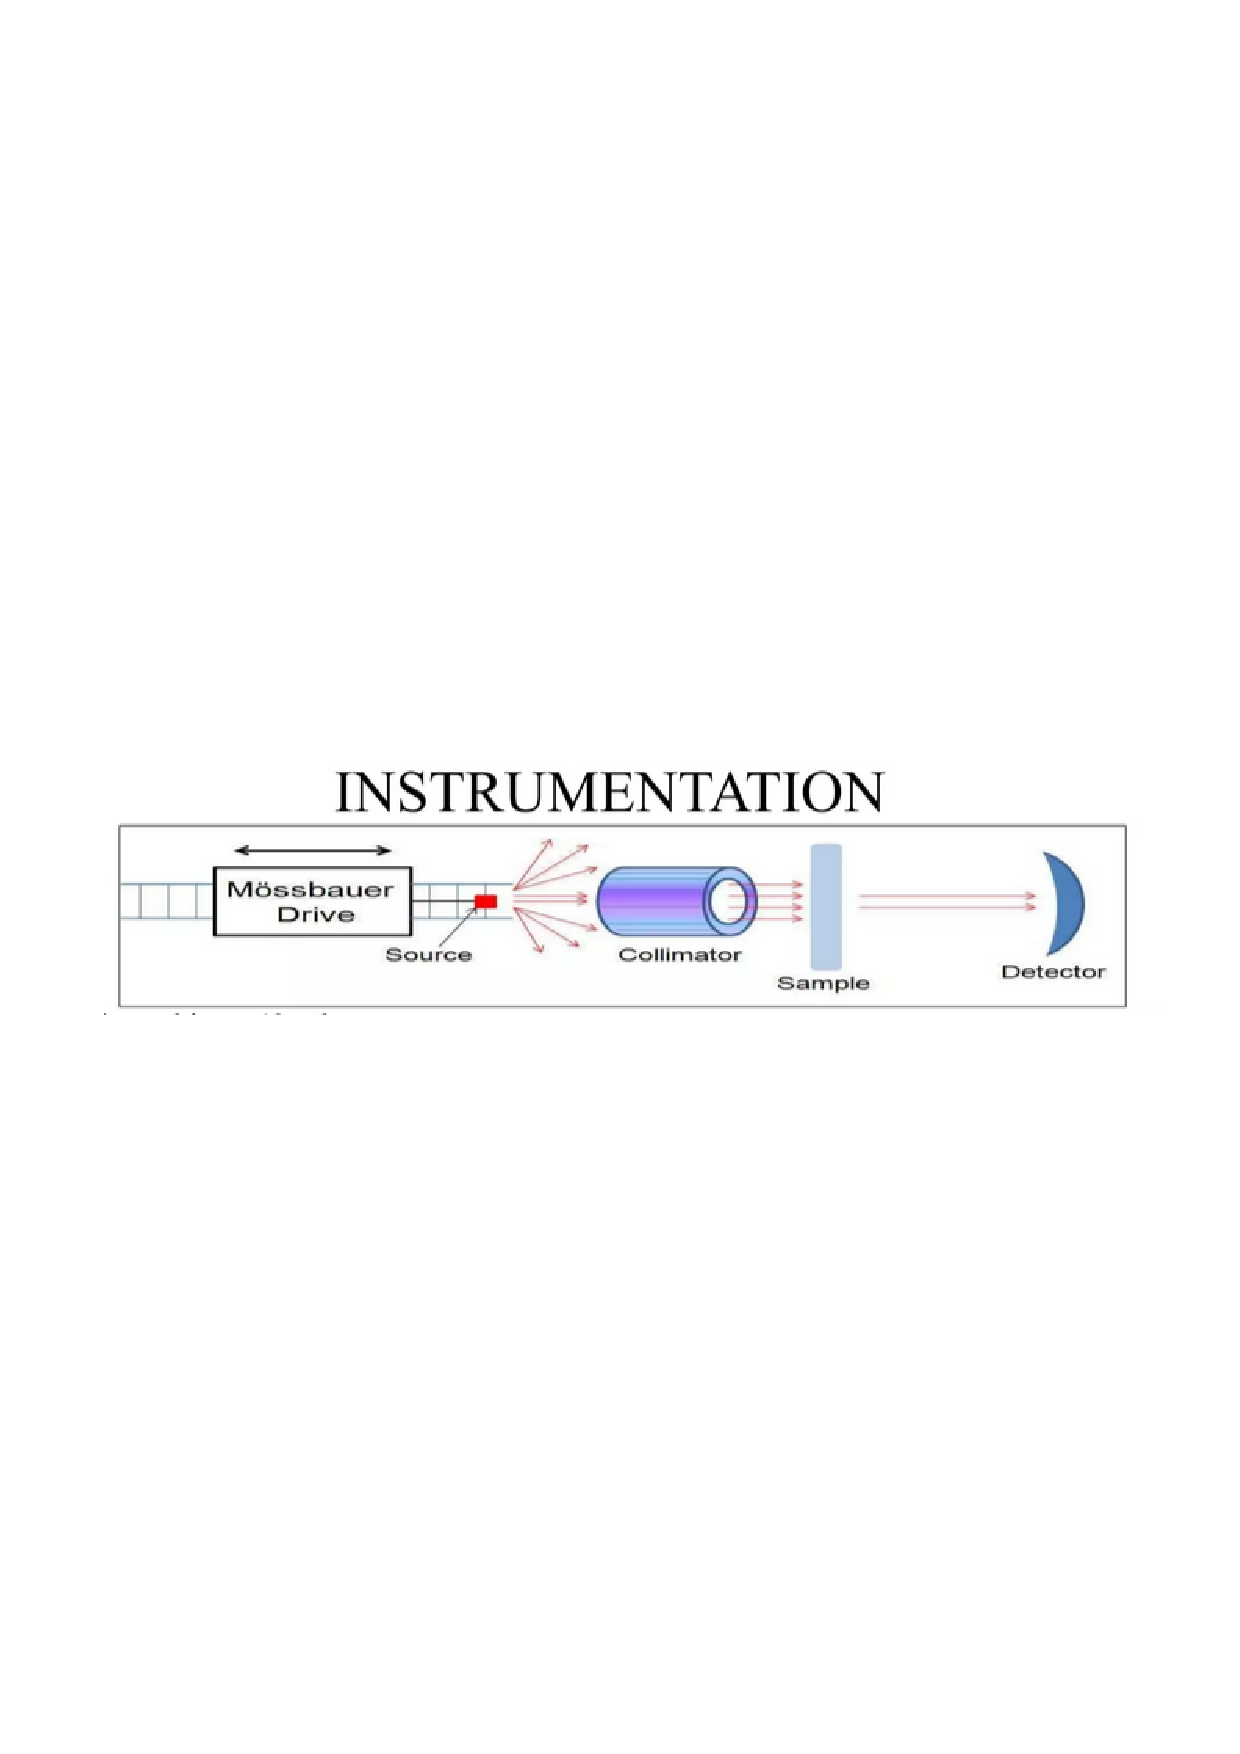
\includegraphics[width=0.8\linewidth, trim={1.5cm 11cm 1.5cm 11cm}, clip]{figs/mossbauer_instrumentation.pdf}
    \caption{Experimentální uspořádání transmisní Mossbauerovy spektrometrie}
    \label{fig:2_6_mossbauer_zapojeni}
\end{figure}

%- můžu mít transmisní geometrii, odrazovou geometrii, můžu měřit konverzní elektrony
%- CEMS (Conversion Electrons Mossbauer Spectroscopy), TMS (Transmission Mossbauer Spectrometr), CXMS (Conversion X-ray Mossbauer Spectroscopy)
%- vzorek nesmí být ani moc tlustý, ani moc tenký - definuji efektivní tloušťku
%- jako detektory se využívají scintilárky, proporcionální detektory, polovodičové detektory nebo Si-PIN detektory
%- scintilační detektory NaI(Tl), YAP(Ce) 
%- proporcionální dteektory mají lepší rozlišení v porovnání se scintilákama
%

\subsubsection{Využití - k čemu je to dobré}
\begin{itemize}
    \item Mossbauerovské jádro mi funguje v mém materiálu jako sonda a říká mi informace o jeho okolí = lokální mikrostruktura
    \item Sledování hyperjmených interakcí Mossbauerovského jádra s jeho okolím = jedná se o interakce, které nějaký způsobem ovlivňují excitační stavy - Energetické stavy budou ovlivňovány svým okolím
    \item Mohu zkoumat vliv např. externího magnetického pole na posun či rozštěpení excitovaného či základního stavu (excitovaný/základní stav mají nějakou hladinu a buď může dojít vlivem externích jevů k jejich posuvu a nebo rozštěpení na více hladit)
    \item Informace o charakteru vazeb
    \item Informace o spinu
    \item Informace o oxidačním stavu
    \item Kvalitativní (identifikace sloučenin) i kvantitativní (poměrové zastoupení) např. fáze železa a jejich poměrové zastoupení i uspořádání. Interakce konkrétního nuklidu se svým okolím. 
    \item Využívá se především v materiálovém výzkumu a dále geologie, farmaceutický průmysl, biologie/medicín. Spíš ale prostě ten materiálový výzkum a je to.
\end{itemize}

\subsubsection{Hyperjemné interakce}

- jedná se o interakce, které nějaký způsobem ovlivňují excitační stavy, a to jak posunem nebo štěpením na více hladin
- bavíme se o:
\begin{itemize}
   \item elektrické monopólové interakci - izomerický posun
   \item elektrická kvadrupólová - kvadrupólové štěpení
   \item magnetická dipólová - magnetické hyperjemné štěpení
\end{itemize}

\begin{figure}[ht!]
   \centering
   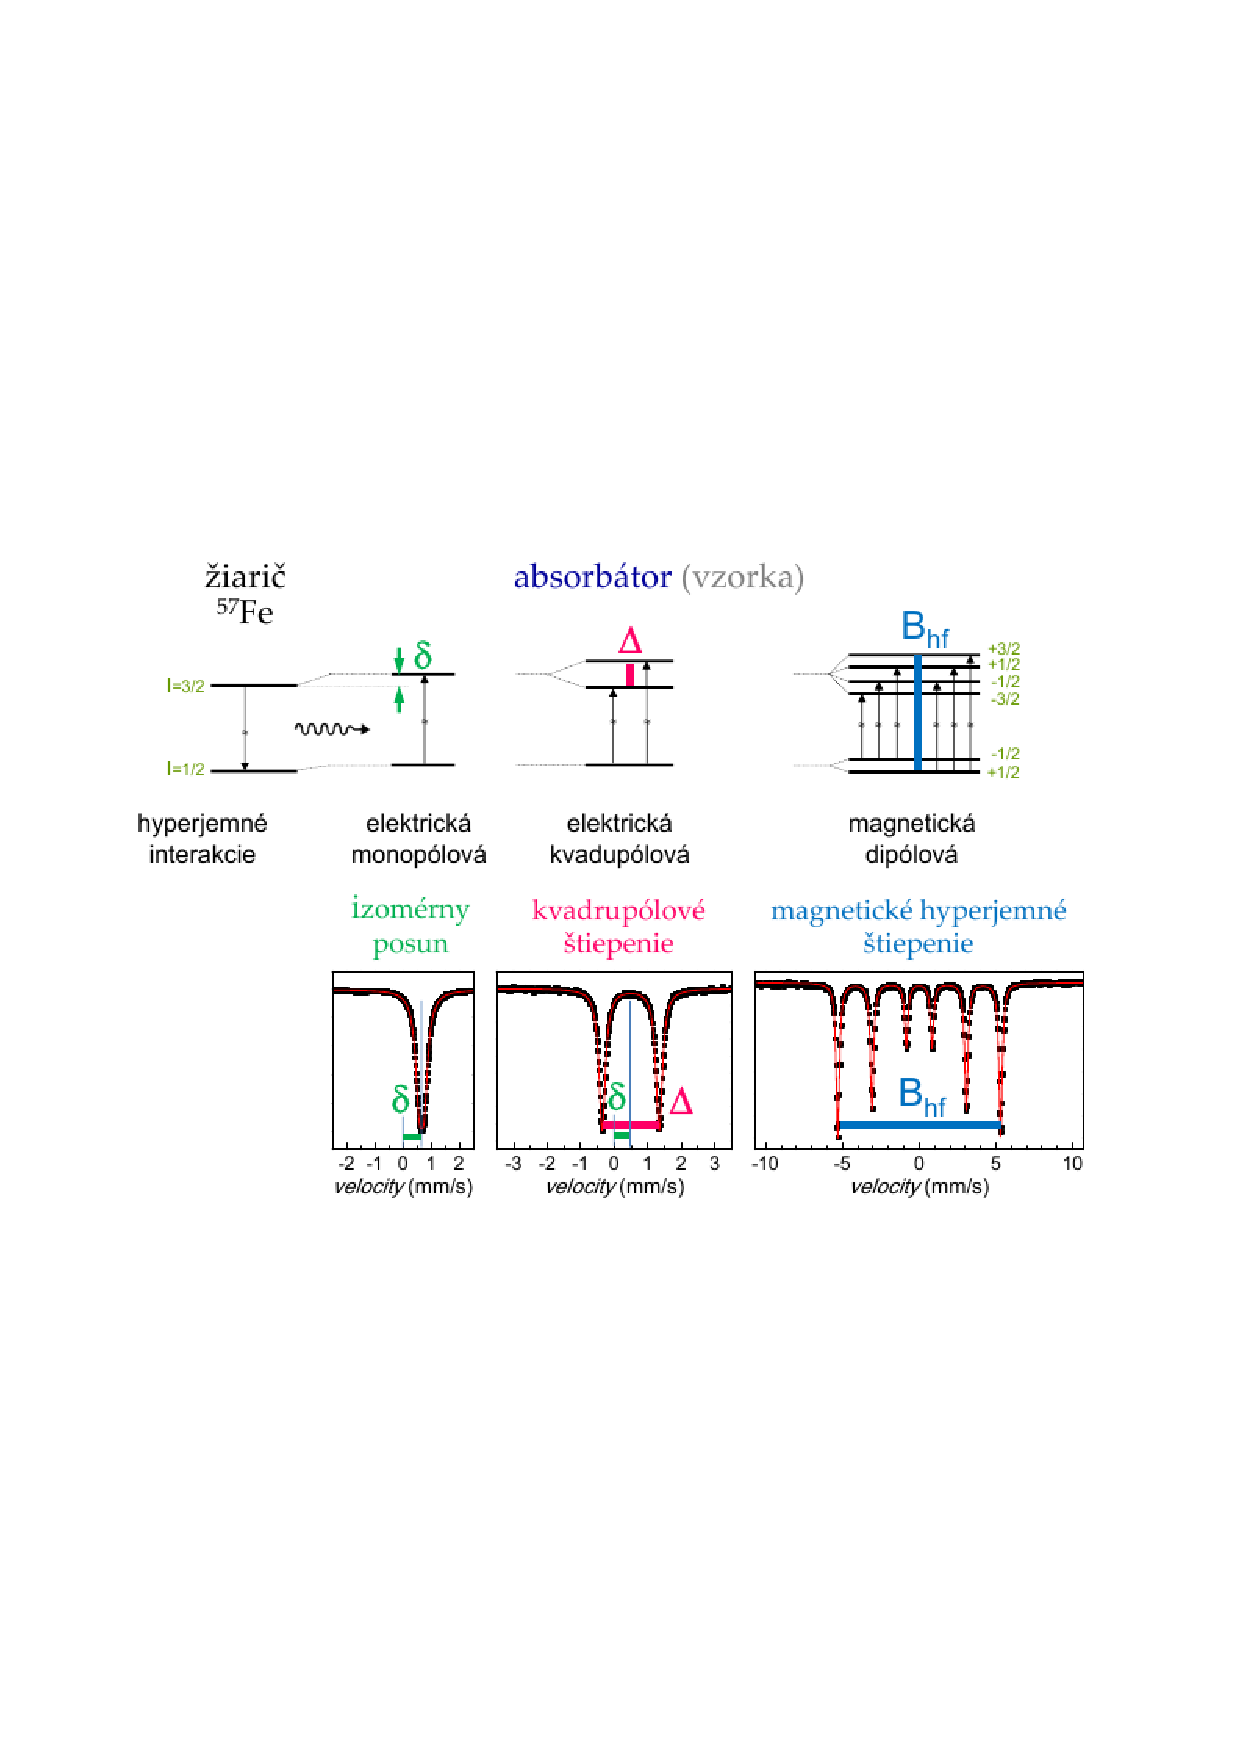
\includegraphics[width=0.8\linewidth, trim={2cm 10cm 2cm 10cm}, clip]{figs/mossbauer_interactions.pdf}
   \caption{Hyperjemné interakce}
   \label{fig:6_2_mossbauer_hyperjemne_interakce}
\end{figure}


\vspace{1 cm}

Elektrická monopólová interakce 
\begin{itemize}
\item interakce rozložení náboje jádra s hustotou elektronů v prostoru jádra 
\item izomerní posun $\delta = \dfrac{2\pi}{5} Ze^2 [R_e^2 - R_g^2] \cdot {\rho_a - \rho_s}$
\item pro excitovaný, resp. základní stav platí, že poloměr jádra se mění, stejně jako hustota
\item určuji s ohledem na referenční materiál (bcc-Fe)
\item udává informacee o charakteru vazeb, spinu, oxidačním čísle, elektronegativitě
\end{itemize}

\vspace{1 cm}
Elektrická kvadrupólová interakce
\begin{itemize}

\item i nterakce mezi jádrovým kvadrupólovým momentem a nehomogenitami elktrického pole
\item kvadrupólové štěpení: $\Delta = \dfrac{1}{2} eV_{zz} (1+\dfrac{1}{3}\eta^2)^{1/2}$ \\
\item jaderná podmínka: elektrický kvadrupólový moment - $eQ \neq$ 0 ($I$ > 1/2) a 
\item elektronová podmínka: gradient elektrického pole od elektronů $\neq$ 0 (příspěvek od mřížky a valenčních elektronů)
\item dává informaci o lókální symetrii, oxidačním stavu, charaktere vazeb, spinovém stavu



\end{itemize}
\begin{figure}[ht!]
   \centering
   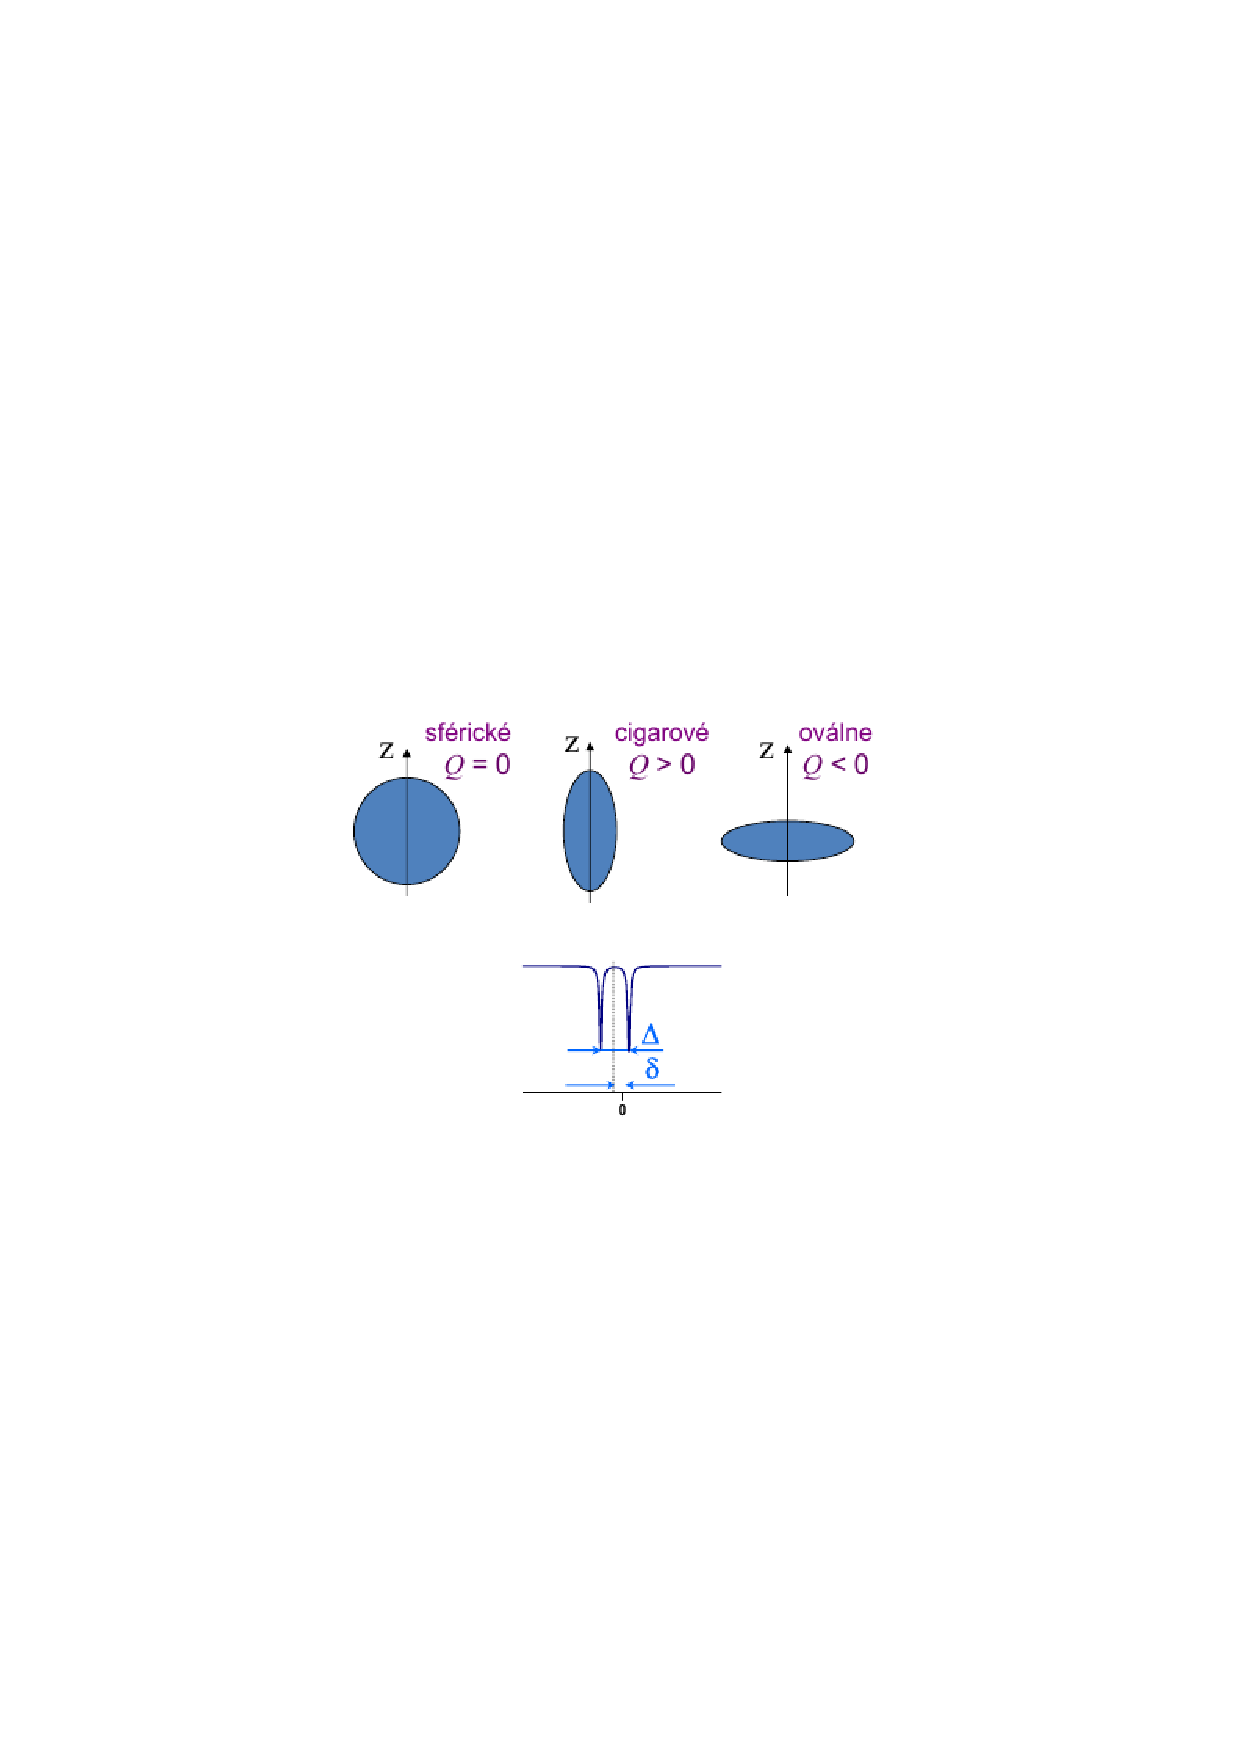
\includegraphics[width=0.5\linewidth, trim={4cm 11cm 4cm 11cm}, clip]{figs/mossbauer_quadrupole.pdf}
   \caption{Elektrické kvadrupólové štěpení}
   \label{fig:6_2_mossbauer_electric_quadrupole}
\end{figure}




\vspace{1 cm}
Magnetická dipólová interakce
\begin{itemize}
   \item interakce magnetického momentu jádra s vnitřním nebo aplikovaným magnetickým polem
   \item $E_{m_1} = - \dfrac{\mu H m_1}{I} = - g_N \beta_N H m_1$
   \item magnetické štěpení hladin jádra (Zeemanův jev)
   \item jádrová podmínka: magnetický dipólový moment $\mu \neq 0$ (I > 0)
   \item elektronová podmínka: intenzita magnetického pole $H \neq 0$
   \item platí výběrová pravidla pro jádrový spin a magnetické kvantové číslo
\end{itemize}
\begin{figure}[ht!]
   \centering
   
\includegraphics[width=0.5\linewidth, trim={5cm 14cm 5cm 14cm}, clip]{figs/mossbauer_magnetic_quadrupole.pdf}
   \caption{Magnetické kvadrupólové štěpení}
   \label{fig:6_2_mossbauer_magnetic_quadrupole}
\end{figure}



\subsubsection{Kalibrace}
\begin{itemize}
   \item zdroj záření: \iso{57}{Co} v matrici Rh, Pd, Cu, Cr
   \item kal%ibrací ryhlostní stupnice (převedu rychlost na energii)
   \item kalibrační absorbátory - bcc-Fe, $\alpha$-Fe$_2$O$_3$
   \item nastvaení nulové rychlosti
\end{itemize}
\subsubsection{APlikace Mossbauerovy spektrometrie}

\begin{itemize}
   \item strukturní informace, stechiometrie, substituce, nekrystalické systém
   \item identifikace fází
   \item Fe2+ a Fe3+
   \item energetické rozlišení 1 : 10$^{13}$
   \item teplotní a tlakové studie
\end{itemize}
\begin{figure}[ht!]
   \centering
   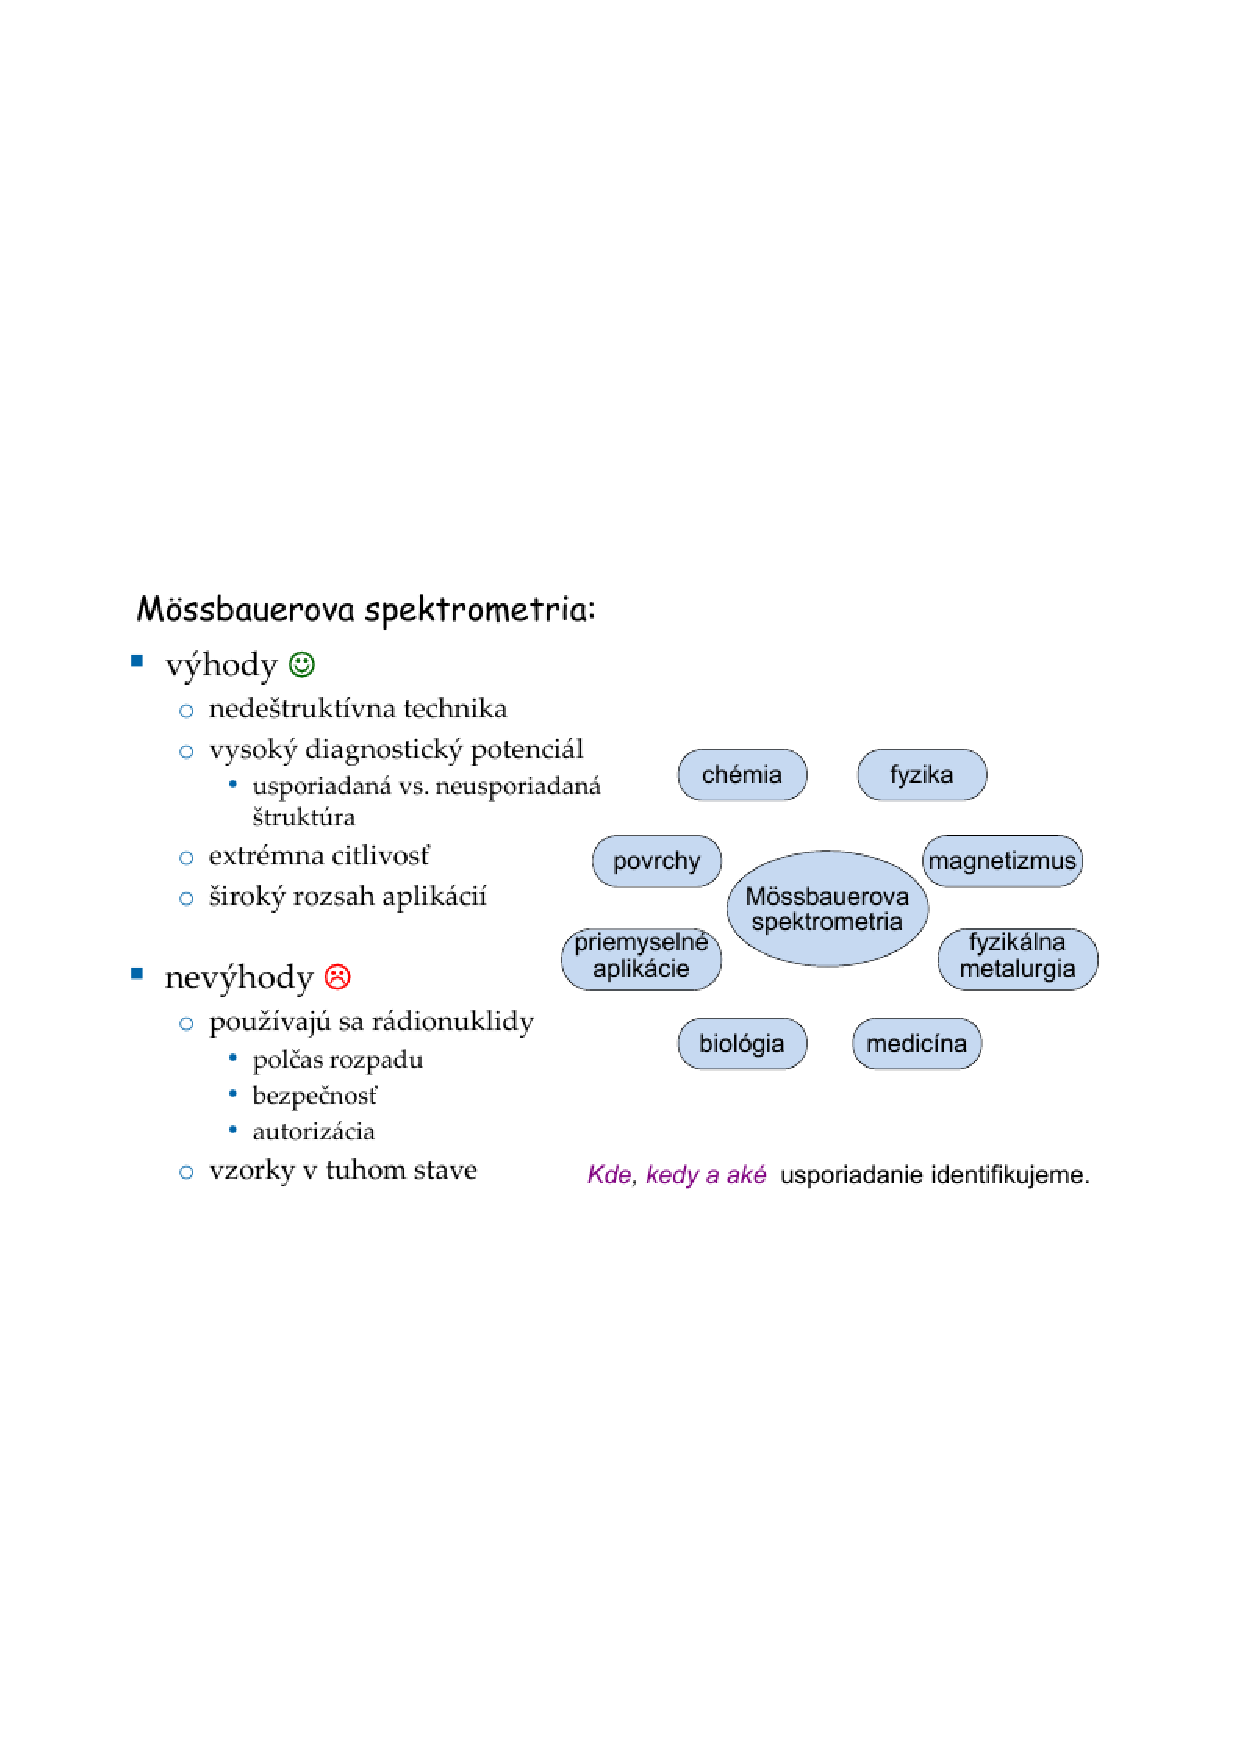
\includegraphics[width=0.5\linewidth, trim={2cm 10cm 2cm 10cm}, clip]{figs/mossbauer_shrnuti.pdf}
\end{figure}


\subsection{Elektron-pozitronová anihilační spektroskopie}
- udává unikátní informace o defektech v pevných látkách (především vakance, dislokace, shluky vakancí, hranice zrn - principiálně se jedná o oblast se sníženou hustotou kladného náboje - od jader :D -> potenciálov jáma pro záchyt pozitronů)

- zdroje pozitronů:
\begin{itemize}
	\item beta+ radionuklidy: jádra bohatá na protony (p -> n + $\beta$ + + $\nu$), Na-22, Cu-64, Co-58
	\item produkce e--e+ párů z vysokoenergetických fotonů gama: impuzní zdroj e+
	\item jaderné reakce: Cd-113(n, gama)Cd-114, Cu-63(n, gama)Cu-64, kontinuální zdroj s vysokou intenzitou
\end{itemize}

-> zdroje pro PET: C-11, N-13, O-15, \textbf{F-18}, Ga-68 - výroba: nejčastěji cyklotron

\noindent- princip anihilace: pozitronový zářič -> interakce pozitronu s elektronem -> vznik dvou fotonů o energii 511 keV (nejpravděpodobnější proce)

\begin{itemize}
    \item anihilace nenastává okamžitě - mezitím: vázaný stav - pozitronium (para a orto pozitronium - podle toho jestli stejný nebo opačný spin pozitronu a elektronu a také podle toho jinak dlouho trvají)
\end{itemize}



\subsubsection{Experimentální techniky}
\begin{itemize}
    \item doba života pozitronů - vyzářen pozitron a gama -> měří se vyzáření pozitornu a gama
    \item Dopplerovo rozšíření  - koincidenční změření energie obou anihilačních fotonů -> charakterizace chem. okolí defektů

    \item úhlové korelace
\end{itemize}

\begin{figure}[ht!]
    \centering
    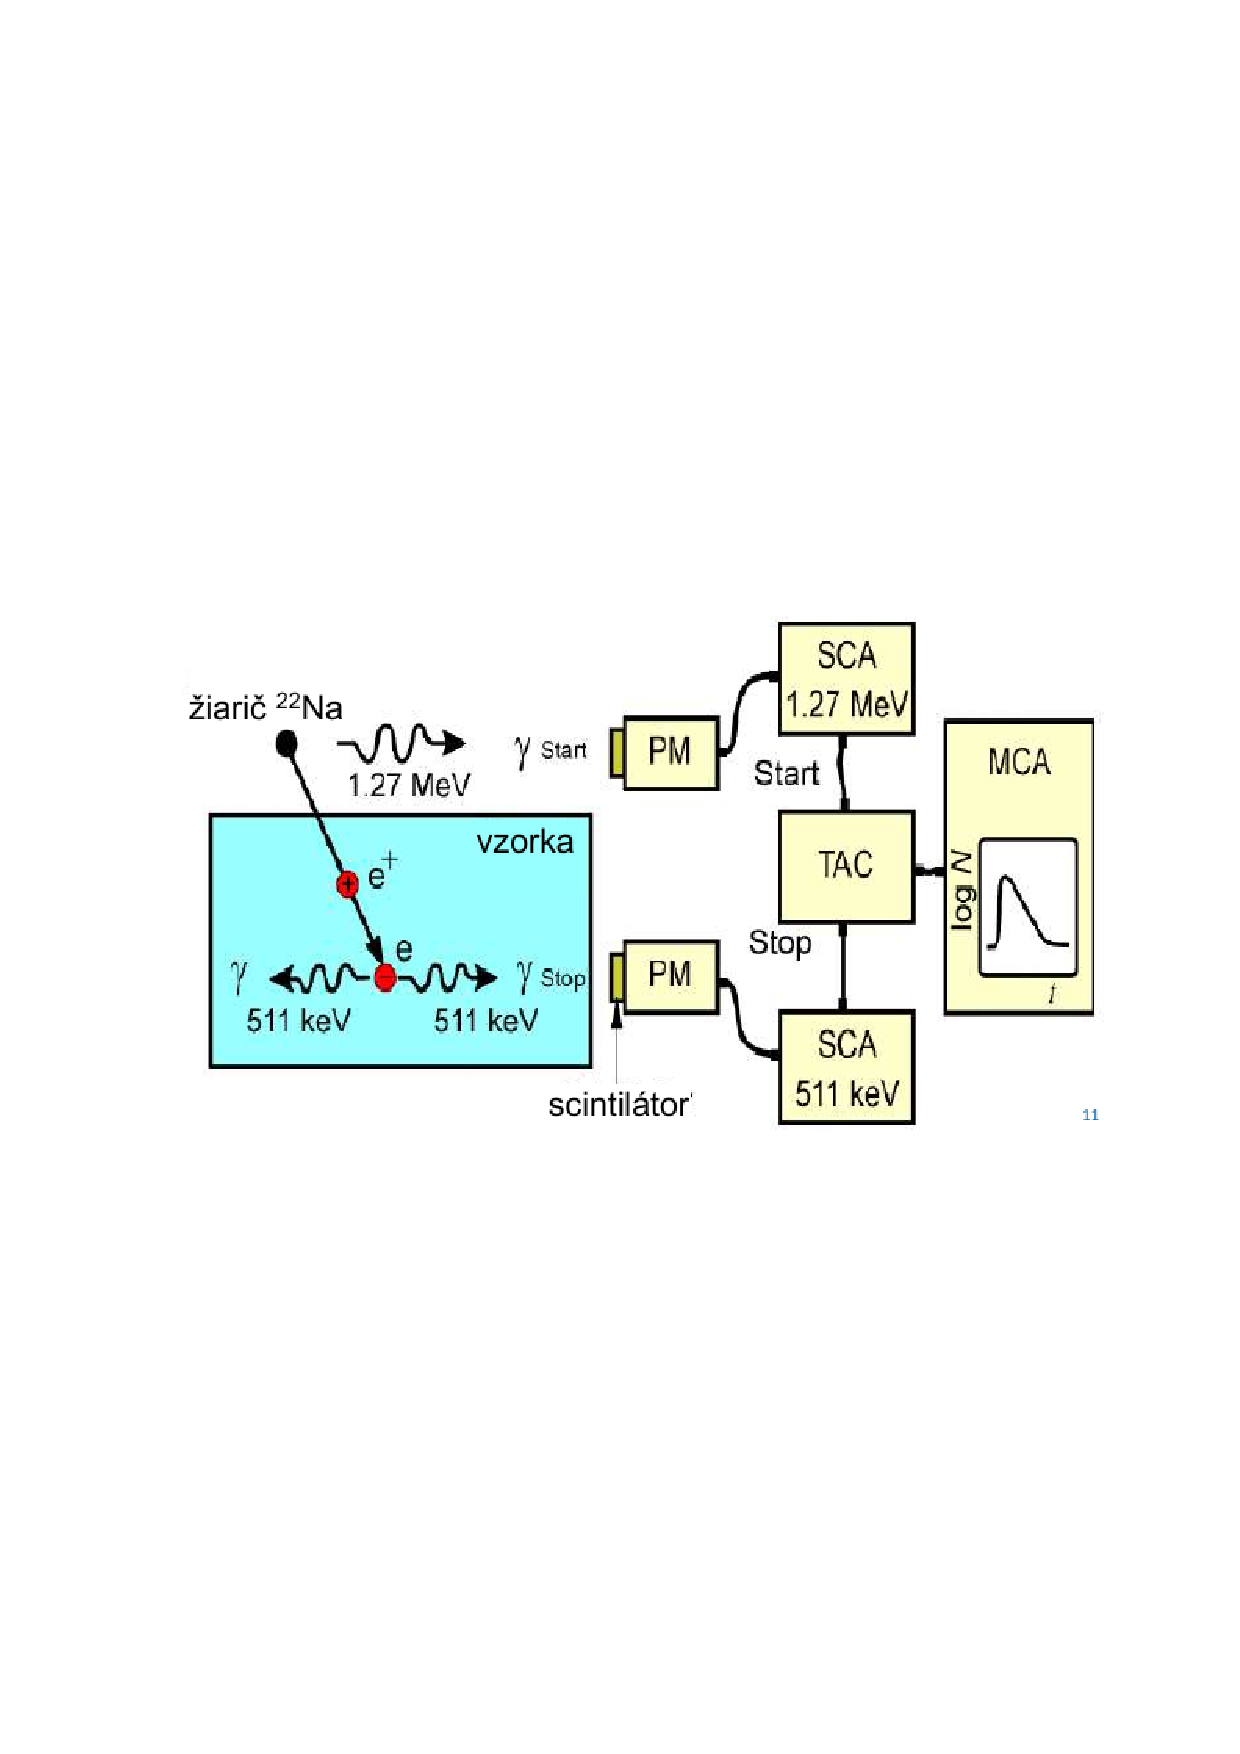
\includegraphics[width=0.8\linewidth, trim={2cm 10cm 2cm 10cm}, clip]{figs/pas_doba_zivota.pdf}
    \caption{Metoda doby života pozitronů.}
    \label{fig:6_2_pas_doba_zivota}
\end{figure}

\begin{figure}[ht!]
    \centering
    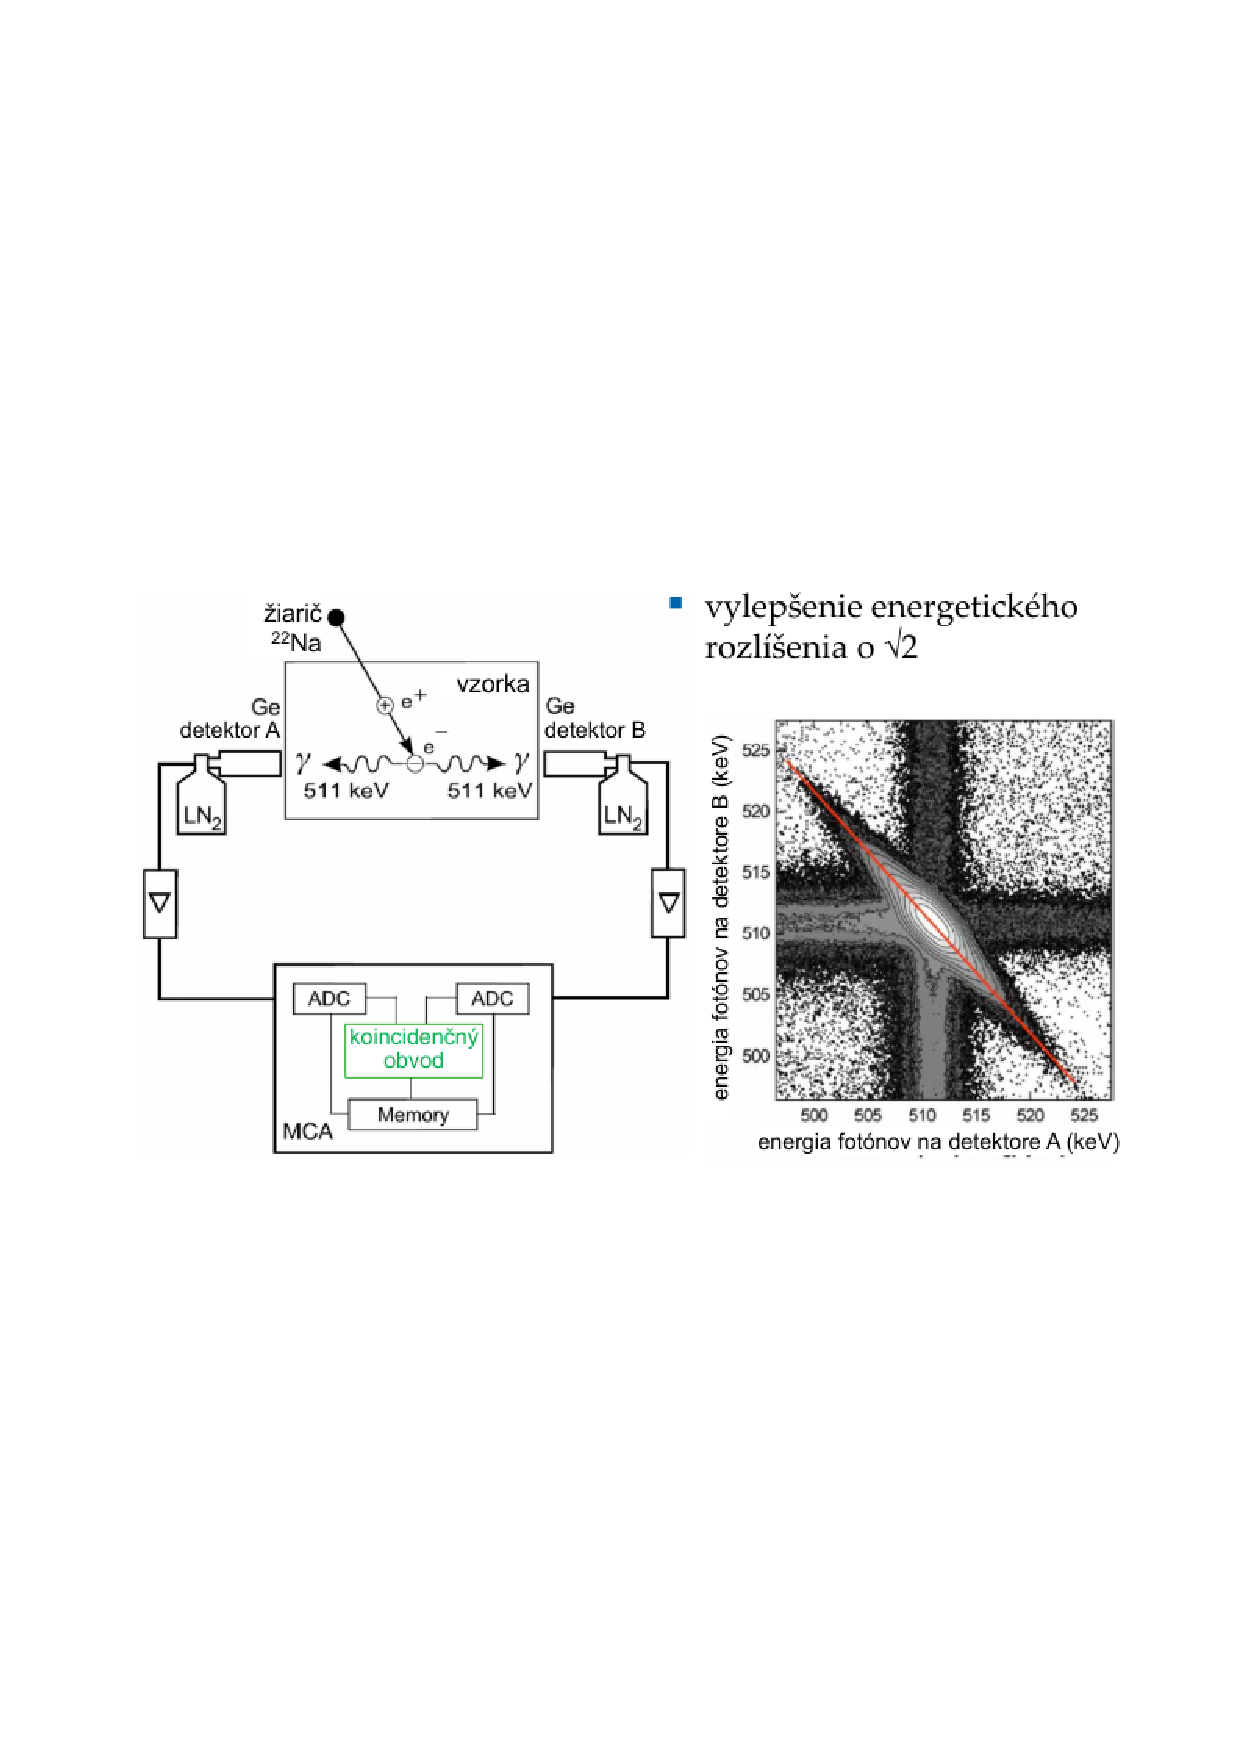
\includegraphics[width=0.8\linewidth, trim={2cm 10cm 2cm 10cm}, clip]{figs/dopplerovo_koincidencni_zapojeni.pdf}
    \caption{Metoda Dopplerova rozšíření- koincidenční zapojení}
    \label{fig:6_2_pas_dopplerovo_rozsireni}
\end{figure}

\subsection{Neutronová aktivační analýza - NAA}

\begin{itemize}
    \item Je založena na aktivaci chemických prvků přítomných v analyzovaném vzorku. 
    \item Jedná se o jednu z nejvíce citlivých metod chemické analýzy
    \item Obvykle je aplikována s využitím měření následného rozpadu aktivovaných prvků (měření gama)
    \item Existuje i metoda s měřením okamžitého záření a ta je využívána pokud produkt reakce má velmi krátký poločas rozpadu a nebo vzniká stabilní produkt.
    \item Pro NAA se dají vyuźít neutrony všech energií, avšak nejčastěji se využívají tepelné, a to kvůli větší dostupnosti neutronů při této energii a také kvůli energetické závislosti účinných průřezů, které mají v této oblasti vysoké hodnoty.
    \item Množství aktivovaných RA atomů daného prvků ve vzorku je přímo úměrné množství těchto atomů a proto se dá využít i pro kvantitativní analýzu.
    \item Indukovaná aktivita závisí na době ozařování a poločasu rozpadu, přičemž okolo $10x T_{1/2}$ dosahuje akivita saturované hodnoty.
    \item Po aktivaci jader v analyzovaném vzorku následuje měření radioaktivity vzorku a identifikace RN na základě energie a intenzity emitovaného gama záření a s ohledem na poločas rozpadu.
    \item Množství studovaného prvku lze získat z naměřené aktivity s tím, že je nutno brát v potaz:
    \begin{itemize}
        \item Hustotu toku neutronů (resp. energetické spektrum)
        \item Energetickou závislost účinných průřezů
        \item Dobu ozařování
        \item Poločas rozpadu
        \item Detekční účinnost trasy (geometrie, stínění, mrtvá doba atd.)
        \item Dobu měření
        \item Dobu chladnutí (přesun po ozařování k detektoru)
    \end{itemize}
\end{itemize}
 
\underline{Rozdělení NAA:}
\begin{itemize}
    \item Absolutní
    
        \begin{itemize}
            \item Z přímého měření aktivity umožňuje stanovit množství zkoumaného izotopu, avšak vyžaduje k tomu přesnou znalost neutronového spektra, účinných průřezů s ohledem na energetický rozsah neutronového pole.
            \item Málo kdy využívaný přístup protože přesná znalost neutronového spektra není v praxi obvykle k dispozici
        \end{itemize}
    \item Porovnávací:
        \begin{itemize}
            \item Srovnávání aktivity RN ve zkoumaném vzorku s jeho aktivitou v podobě standardu/etalonu o známé hmotnosti a složení, který byl ozářen za stejných podmínek jako zkoumaný vzorek
            \item Při srovnávací metodě se nevyužívají hodnoty účinných průřezů ani neutronový tok a v případě stejné geometrie při detekci/měření tak ani absolutní detekční účinnost (pro oba měřené je to stejné, tak to není vyžadováno)
            \item Vysoká přesnost, avšak časově náročné pokud vzorek obsahuje vícero prvků, protože pro každý je nutné mít etalon zvlášť.

        \end{itemize}
    \item $k_0$ metoda
        \begin{itemize}
            \item využívá $k_0$ faktory, které se stanovují na základě jaderných dat v kombinaci s experimentálním stanovením.
            \item nezávisí na neutronovém toku a charakteristikách detektoru
        \end{itemize}
    \item Instrumentální NAA - toto známe a děláme na KJR.
        \begin{itemize}
            \item Nedestruktivní metoda pro stanovení vícero prvků v rámci jednoho měření
            \item Nežádoucím efektem je vzájemné ovlivňování prvků = Vznik jednoho RN reakcemi na dvou různých prvcích (26Mg(n;$\gamma$)27Mg a 27Al(n;p)27Mg) = Tento problém je ovšem řešitelný v případě, kdy jeden z prvků produkuje i další radioaktivní nuklidy a dále také pokud je rozdíl v energetické závislosti účinných průřezů na energii neutronů, tak se dá použít vhodný filtr jako např Cd.
            \item V praxi se měří tak, že se vzorek ozáří v reaktoru na saturovanou hodnotu, pak se nechá vychladnout (snížení aktivity) pokud je moc naaktivovaný a pak se odnese do gama spektrometru a měří se gama záření z rozpadu RN. Z naměřeného spektra se poté stanovuje kvantita a kvalita složení materiálu.
        \end{itemize}
\end{itemize}

\subsubsection{Nastavení experimentálních parametrů}
\begin{itemize}

            \item V rámci tohoto měření, tak je vhodné mít odladěnou dobu ozařování (ať to není zbytečně moc a aktivita dlouhodobě žijících RN není moc vysoká)
            \item dobu vymření (chceme minimalizovat aktivitu všech RN kromě toho, který chceme měřit)
            \item Doba měření (měla by být kratší než nějaký významnější pokles aktivity vzorku - pak mi do toho začne hrát roli pozadí a Rn, K a U)
            \item při ozařování dochází ke vzniku vícero aktivačních produktů z jednoho prvku (pro ověření lze měřit dlouho a zaměřit se na ověření přes poločas rozpadu). Popřípadě aktivační produkty obvykkle emitují $\gamma$ fotony o vícero energiích, čímž je možné taky jednoznačně stanovit.
            \item Měřící geometrie (mrtvá doba)
            \item Velikost vzorku: zbytečně velký vzorek představuje riziko samostínění, samoabsorpce gama záření či zbytečně velkou aktivitu nebo problematické manipulace (to platí i pro zbytečně malý vzorek).
            \item Tok primárních částic přímo ovlivňuje úroveň produkované aktivity.
            \item Ve výsledném výpočtu reakční rychlosti, resp. obecně měření je nutné zohlednit několik faktorů = plocha pod píkem při měření, počet částic v látce na počátku, oprava na čistou dobu měření, doba ozařování, rozpad při vymírání, rozpad při měření, Radiační výtěžek (oprava na intenzitu gama přechodu), oprava na efektivitu detektoru pro danou geometrii (detekční účinnost). Korekce na nerovnoměrné ozařování, korekce na samoabsorpci.
        \end{itemize}

\underline{Využití a aplikace NAA:}
\begin{itemize}
    \item Monitoring životního prostředí
    \item Zajištění jakosti v průmyslu
    \item Hygienické studie
    \item Certifikace referenčních materiálů
    \item Stopové prvky
    \item Kvalita půdy
    \item Analýza prvkového složení
    \item Analýza uhlí
    \item Mnohé další
\end{itemize}

\newpage
\section{Jaderně fyzikální metody v nukleární medicíně (gamma kamera, CT, PET)}
Jedná se o metody založené na využití farmaceutických radionuklidů, a to ve formě absorpce v těle nebo zavedenímm do lidského organismu. Jako detektory jsou většinou využívány scintilátory, proto metody dělíme na:
\begin{itemize}
    \item dynamickou scintilografii - sleduje časové změny rozložení radionuklidů, např. činnost orgánů
    \item planární scintilografie - statická vizualizace
\end{itemize}
\subsection{Zdroje záření}
V medicíně lze využívat růzzné druhy zdrojů:

\begin{itemize}
    \item radionuklidy 
    \begin{itemize}
        \item $\gamma$ záření z jaderných reakcí, jsou definovány energií a poločasem rozpadu, musí být vyráběny např. na cyklotronech
        \item \iso{99m}{Tc} - $\gamma$-kamery, \iso{18}{F} - PET, \iso{123}{I} - $\gamma$ kamera, \iso{131}{I} - terapeutický zdroj (prostě ti to vysmaží mutující buňky v nádoru), \iso{11}{C} - PET, \iso{67}{Ga} - $\gamma$ kamera, \iso{81}{Rb} - PET \textit{každý ten zdroj se používá na něco trochu jiného, na diagnostiku mozku použijí asi nějaký jiný než na diagnostiku sleziny atd.}
        
    \end{itemize}
\end{itemize}

\subsection{Diagnostika}

Dělíme podle činnosti:
\begin{itemize}
    \item morfologická (uspořádání, tvar, velikost)
    \item funkční (činnost orgánů)
    \item dynamická (časová závislost)
\end{itemize}
podle uspořádání:
\begin{itemize}
    \item absorpční - RTG, CT
    \item emisní - PET, gamma kamera, magnetická rezonance
    \item kombinovaná - NAA, CT+PET
    
\end{itemize}

\subsection{Gamma kamera}

\begin{figure}[ht!]
    \centering
    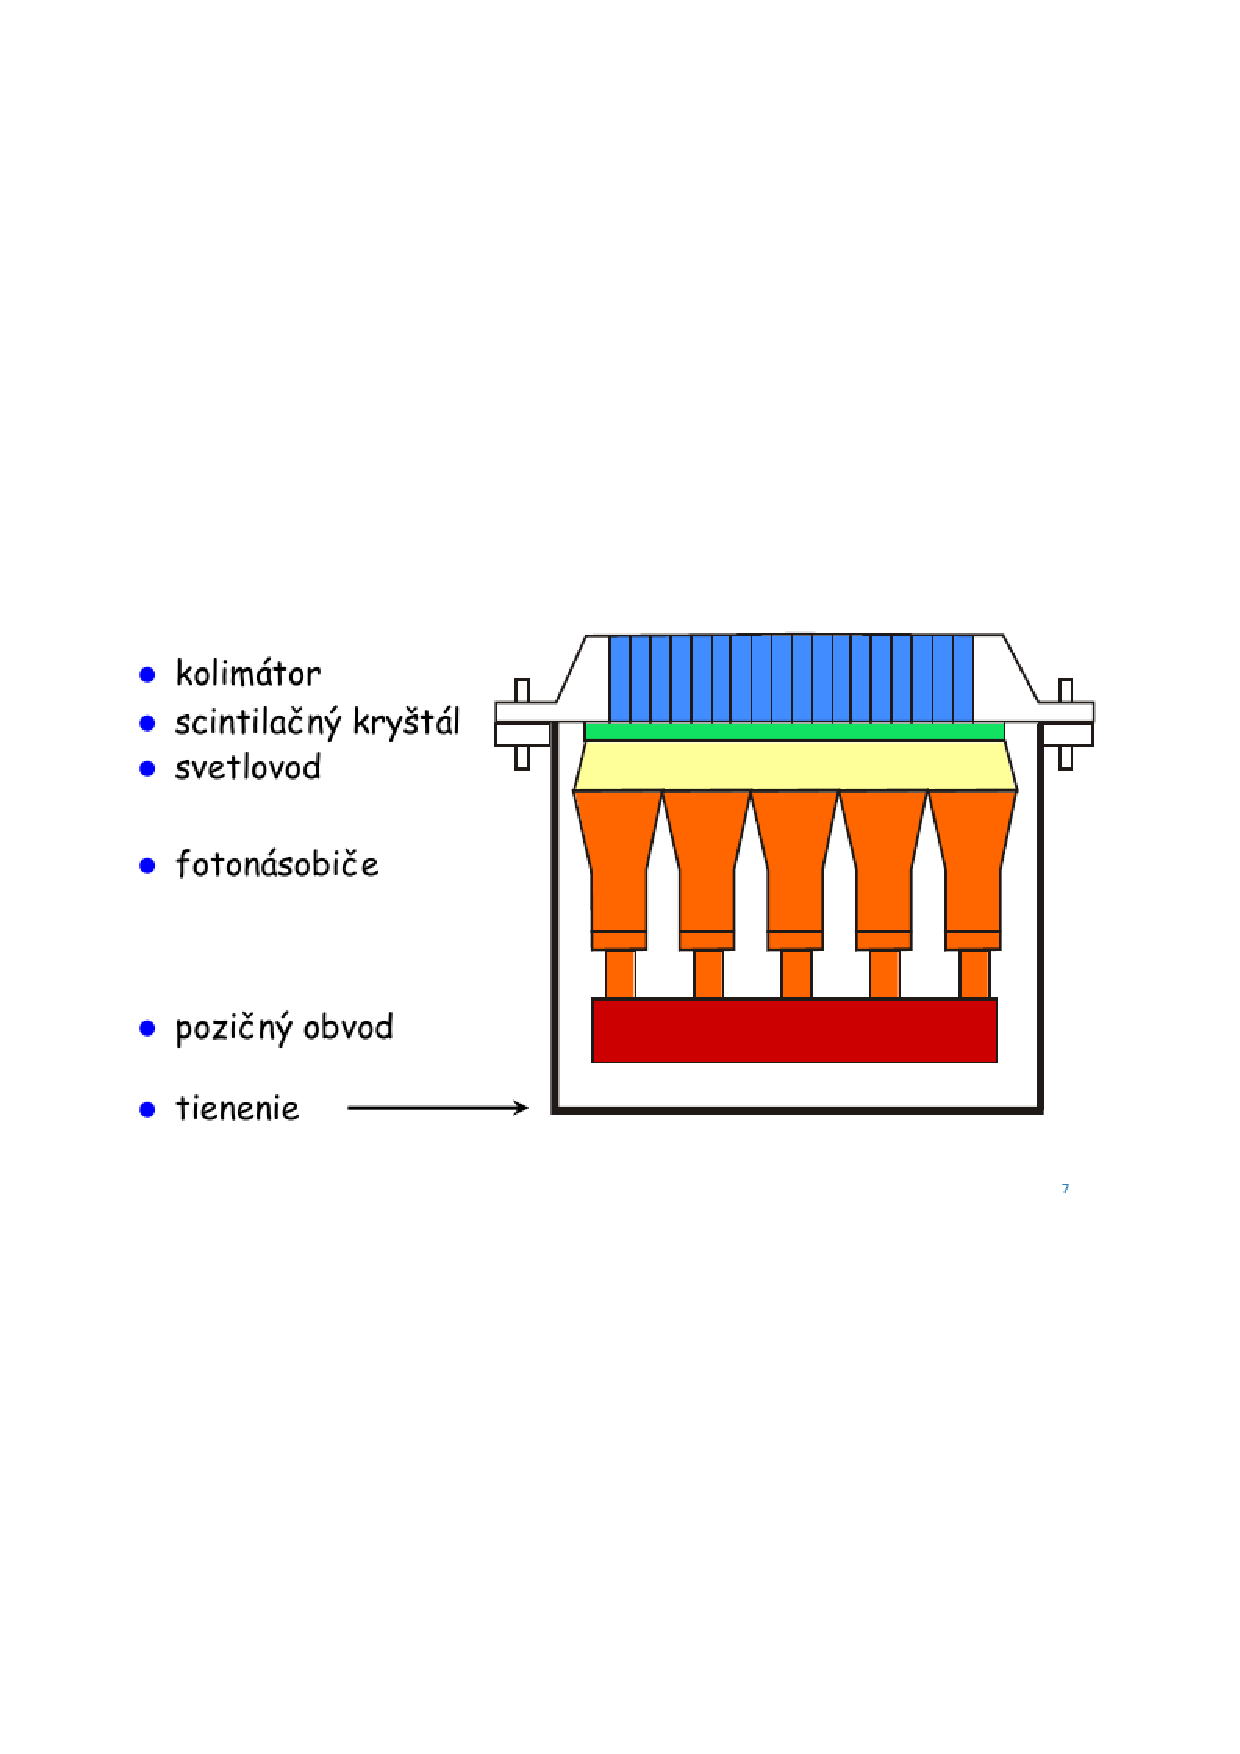
\includegraphics[width=0.55\linewidth, trim={2cm 10cm 2cm 10cm}, clip]{figs/gamma_kamera.pdf}
    \caption{Základní komponenty gamma kamery}
    \label{fig:2_5_gamma_kamera}
\end{figure}

\begin{figure}[ht!]
    \centering
    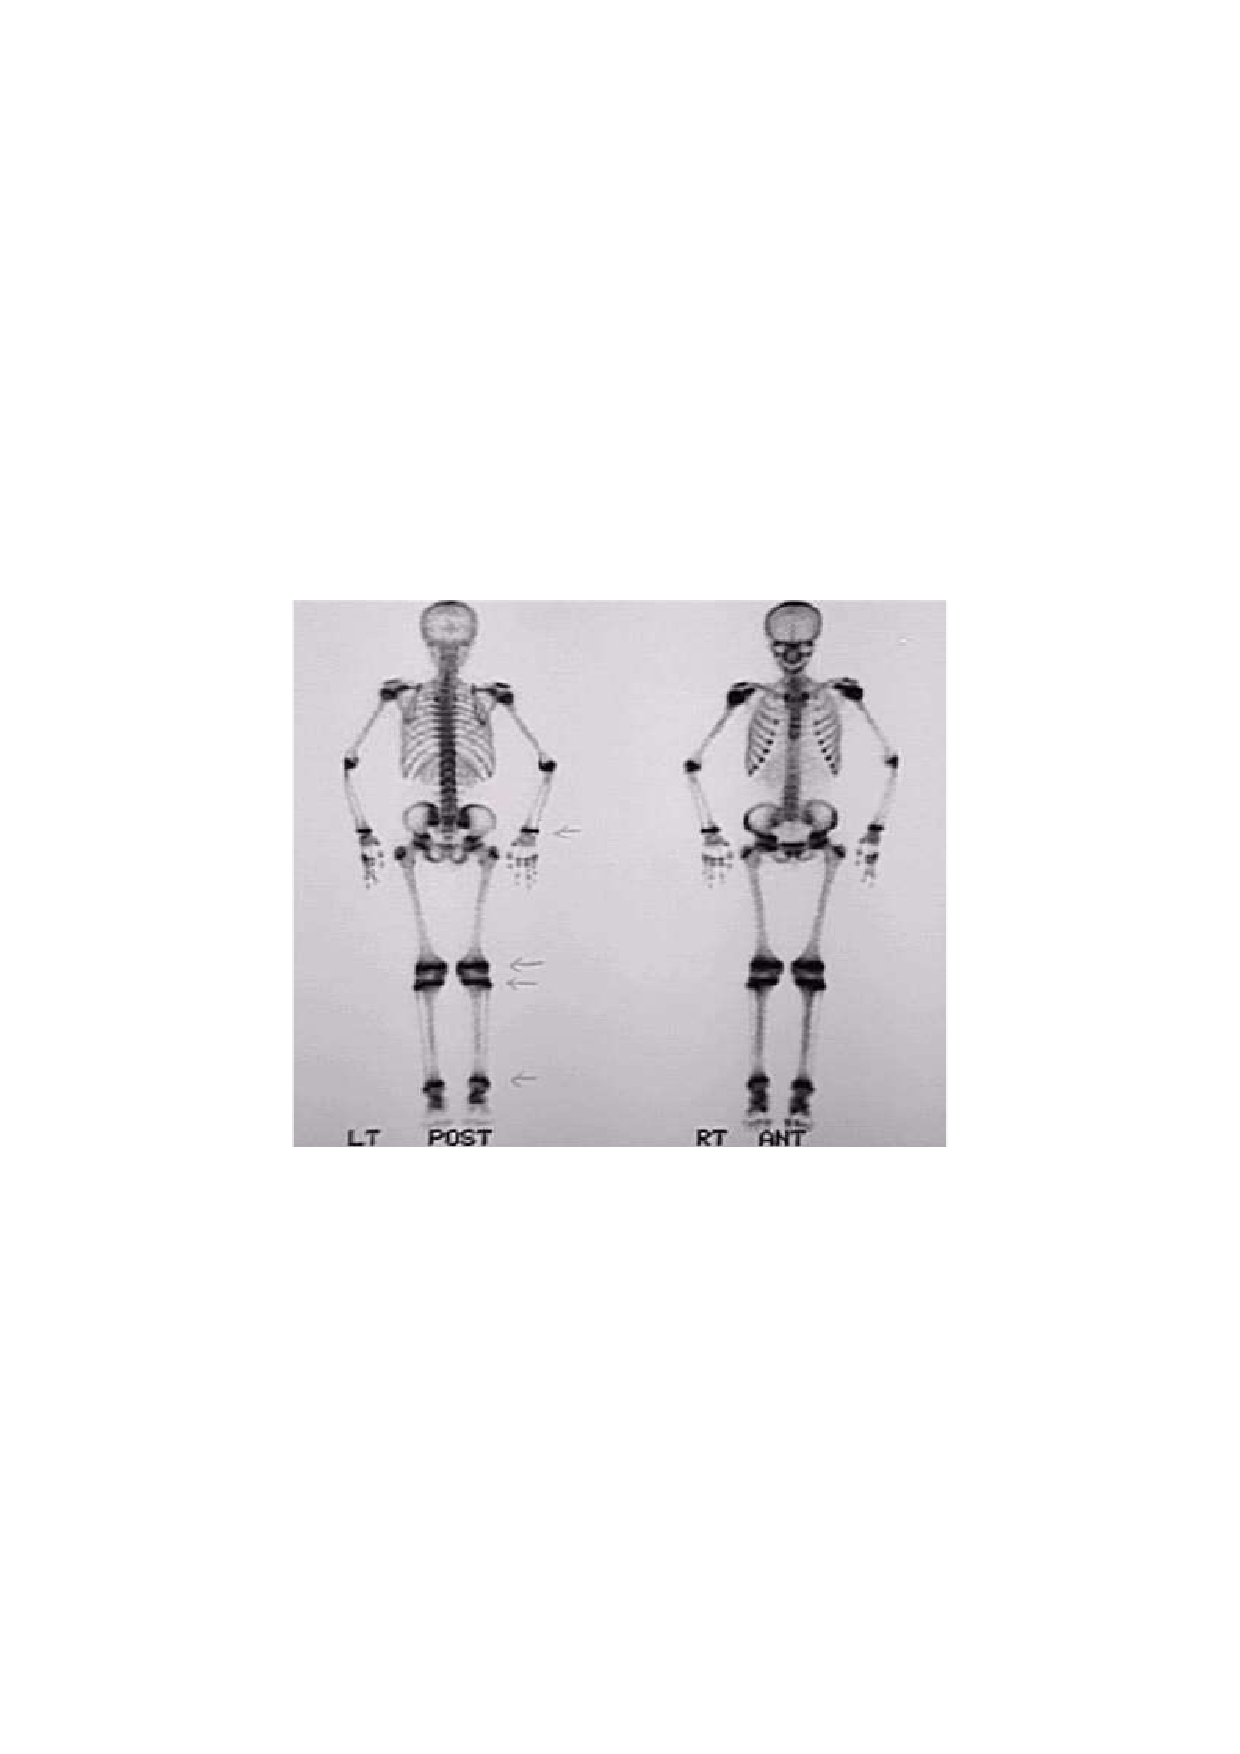
\includegraphics[width=0.5\linewidth, trim={2cm 8cm 2cm 8cm}, clip]{figs/gamma_kamera_snimek.pdf}
    \caption{Celotělový snímek z gamma kamery}
    \label{fig:5_2_gamma_kamera_snimek}
\end{figure}
Kolímátor: 
\begin{itemize}
    \item paralelní mnohokanálový kolimátor - ovlivní směr fotonů, geometické zorné pole kamery, prostorov rozptyl, citlivost systému - výběr dle energie registrovaných fotonů, rozlišení, skenovací hloubky a požadované citlivosti
    \item výsledný obraz - počet otvorů, průměr otvorů, délka jednotlivých trubic, materiál atd.
\end{itemize}
Výběr radionuklidu:
\begin{itemize}
    \item poločas rozpadu musí mít několik hodin, produkované $\gamma$ musí ít stovky keV, lehko zabudovatelný do farmaka, v nemocnici musí vydržet několik dní
    \item typicky se používá \iso{99m}{Tc}
\end{itemize}


\subsection{Počítačová tomografie - CT}
\subsubsection{Princip}
- založená na zeslabení svazku RTG záření (absorpční metoda)
- RTG: $I = I_0 \cdot exp(-\mu\cdot t)$
- CT: mám sadu $j$ řádků a $i$ sloupců, každý detektor sbírá informaci o zeslabení
$$I_{12} = I_{0} \cdot exp(-(\mu_{1} + \mu_{2})\cdot \Delta t)$$
$$I_{34} = I_{0} \cdot exp(-(\mu_{3} + \mu_{4})\cdot \Delta t)$$
$$I_{13} = I_{0} \cdot exp(-(\mu_{1} + \mu_{3})\cdot \Delta t)$$
$$I_{24} = I_{0} \cdot exp(-(\mu_{2} + \mu_{4})\cdot \Delta t)$$

- přes získané intenzity $I_{12}, I_{34}, I_{13}, I_{24}$ jsem schopný zrekonstruovat koeficienty $\mu_{i}$ ve všech blocích

-takhle to funguje, akorát je těch bloků o dost více


- generované RTG záření prochází tělem, na druhé straně gantry jsou detekován sadou scintilátorů

- získané data tvoří projekci, kompletní sada zeslabení v závislosti na úhlu $\theta$ a vzdálenosti $t$ je pak sinogram

- následně je obraz rekonstruován 

- sinogram je kompletní soubor projekcí, ukazuje grafickou závislost polohy objektu od úhlu projekce
\begin{figure}[ht!]
    \centering
    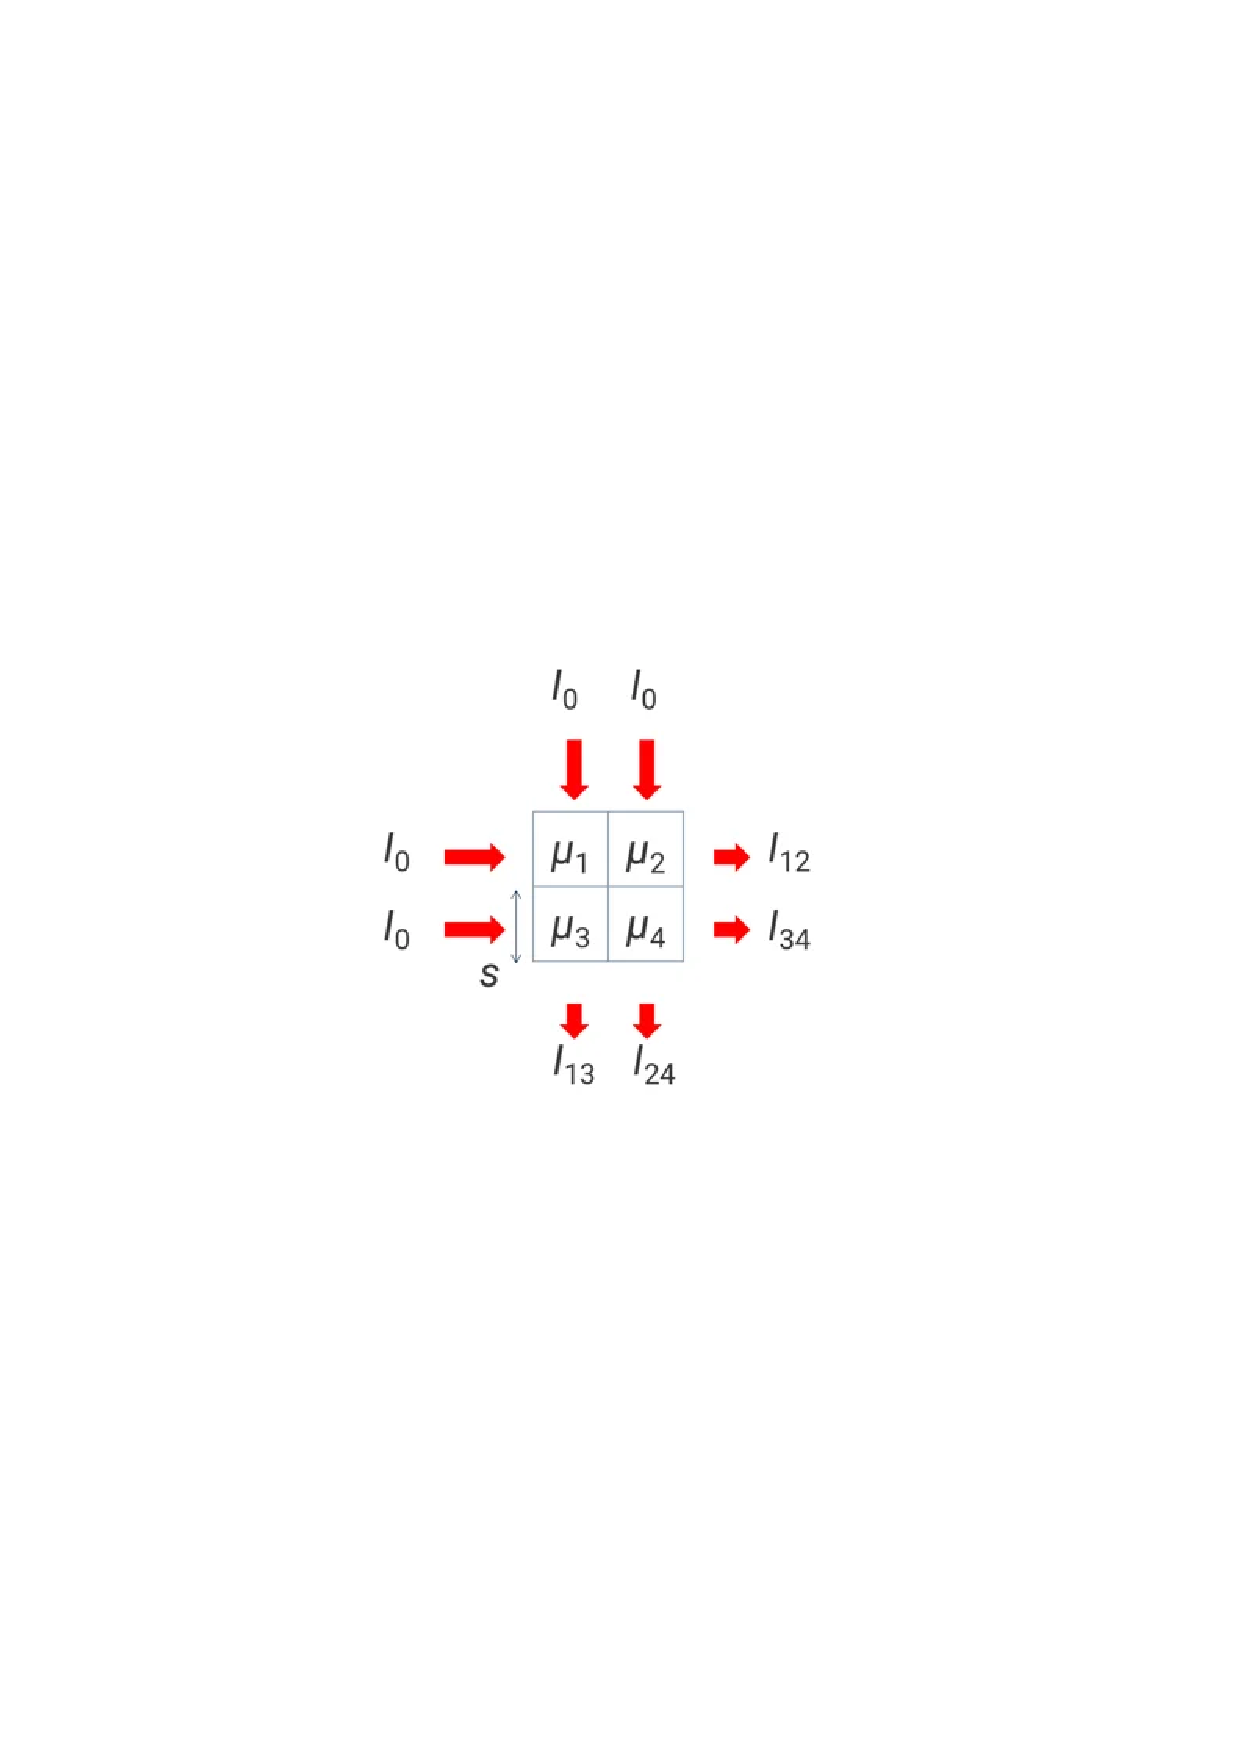
\includegraphics[width=0.4\linewidth,trim={5cm 10cm 5cm 10cm}, clip]{figs/ct_scheme.pdf}
    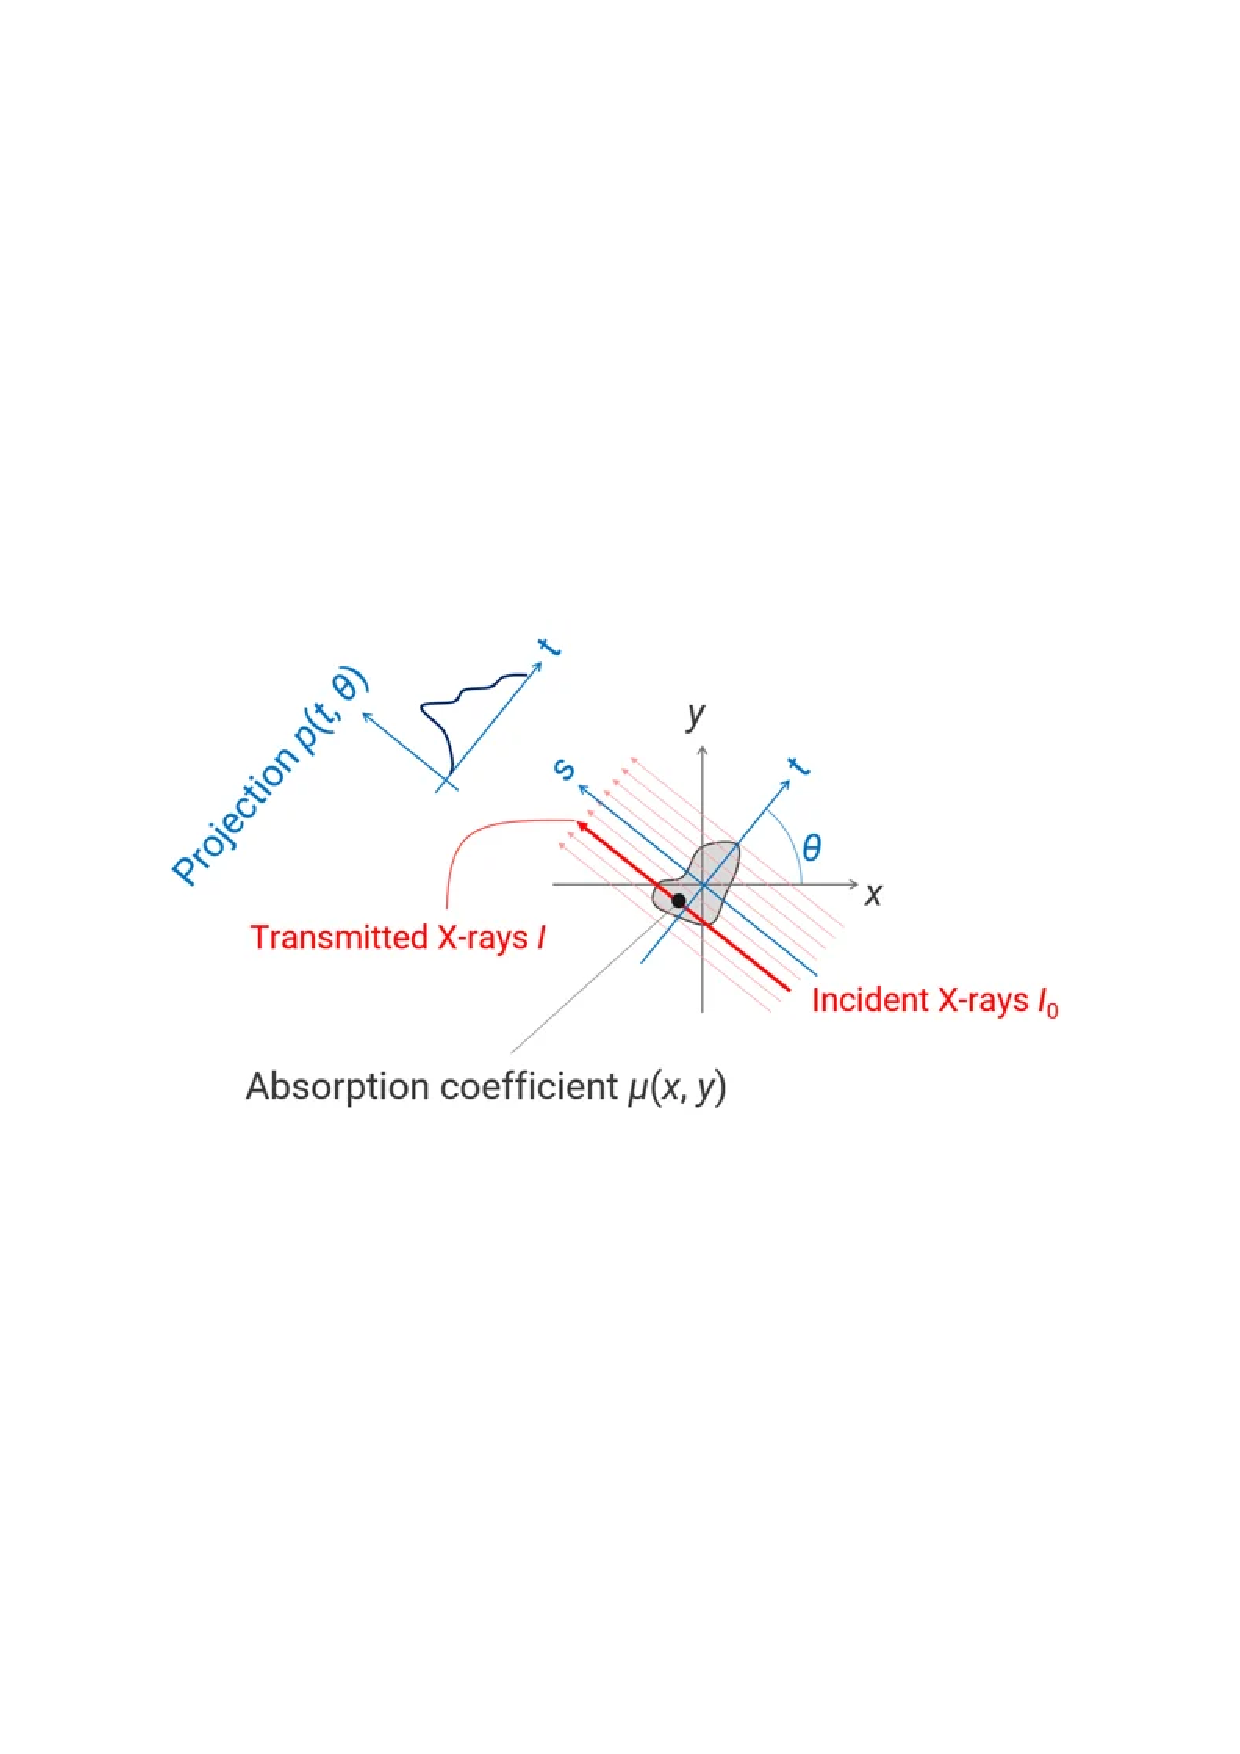
\includegraphics[width=0.5\textwidth,trim={2.5cm 10cm 3cm 10cm}, clip]{figs/ct_projection.pdf}
    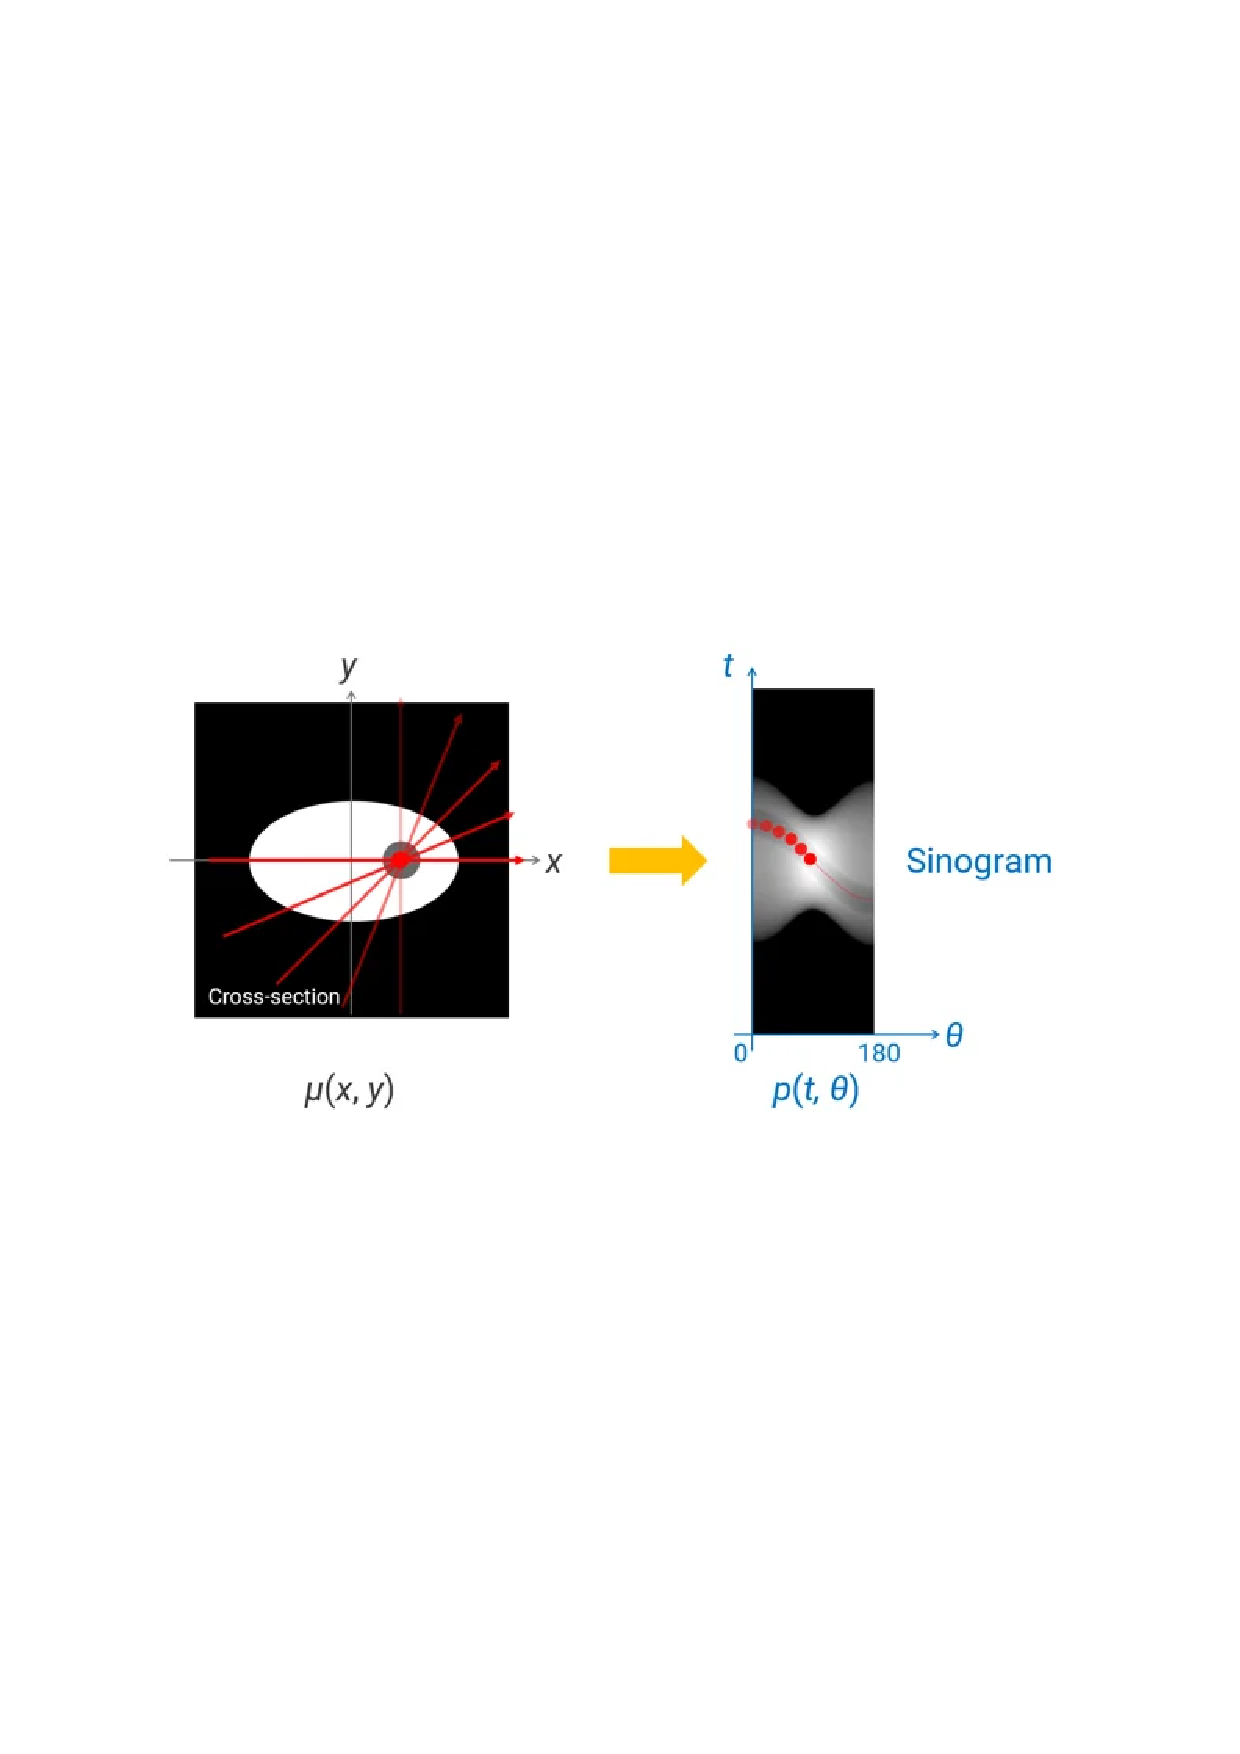
\includegraphics[width=0.5\textwidth,trim={3cm 7cm 3cm 10cm}, clip]{figs/ct_sinogram.pdf}
    
\end{figure}
- kontrast se hodnotí vůči koeficientu zeslabení pro vodu, jednotky Hounsfield
- pokud budu proces opakovat a posouvat spirálou axiálně podél těla $\longrightarrow$ dostanu 3D obraz


\subsubsection{Základní součástky CT tomorgafu}
\begin{itemize}
    \item gantry, RTG trubice, kolimátor a filtr, detektory, systém získávání informací o odezvě, vyšetřovací lůžko
\end{itemize}
\begin{figure}[ht!]
    \centering
    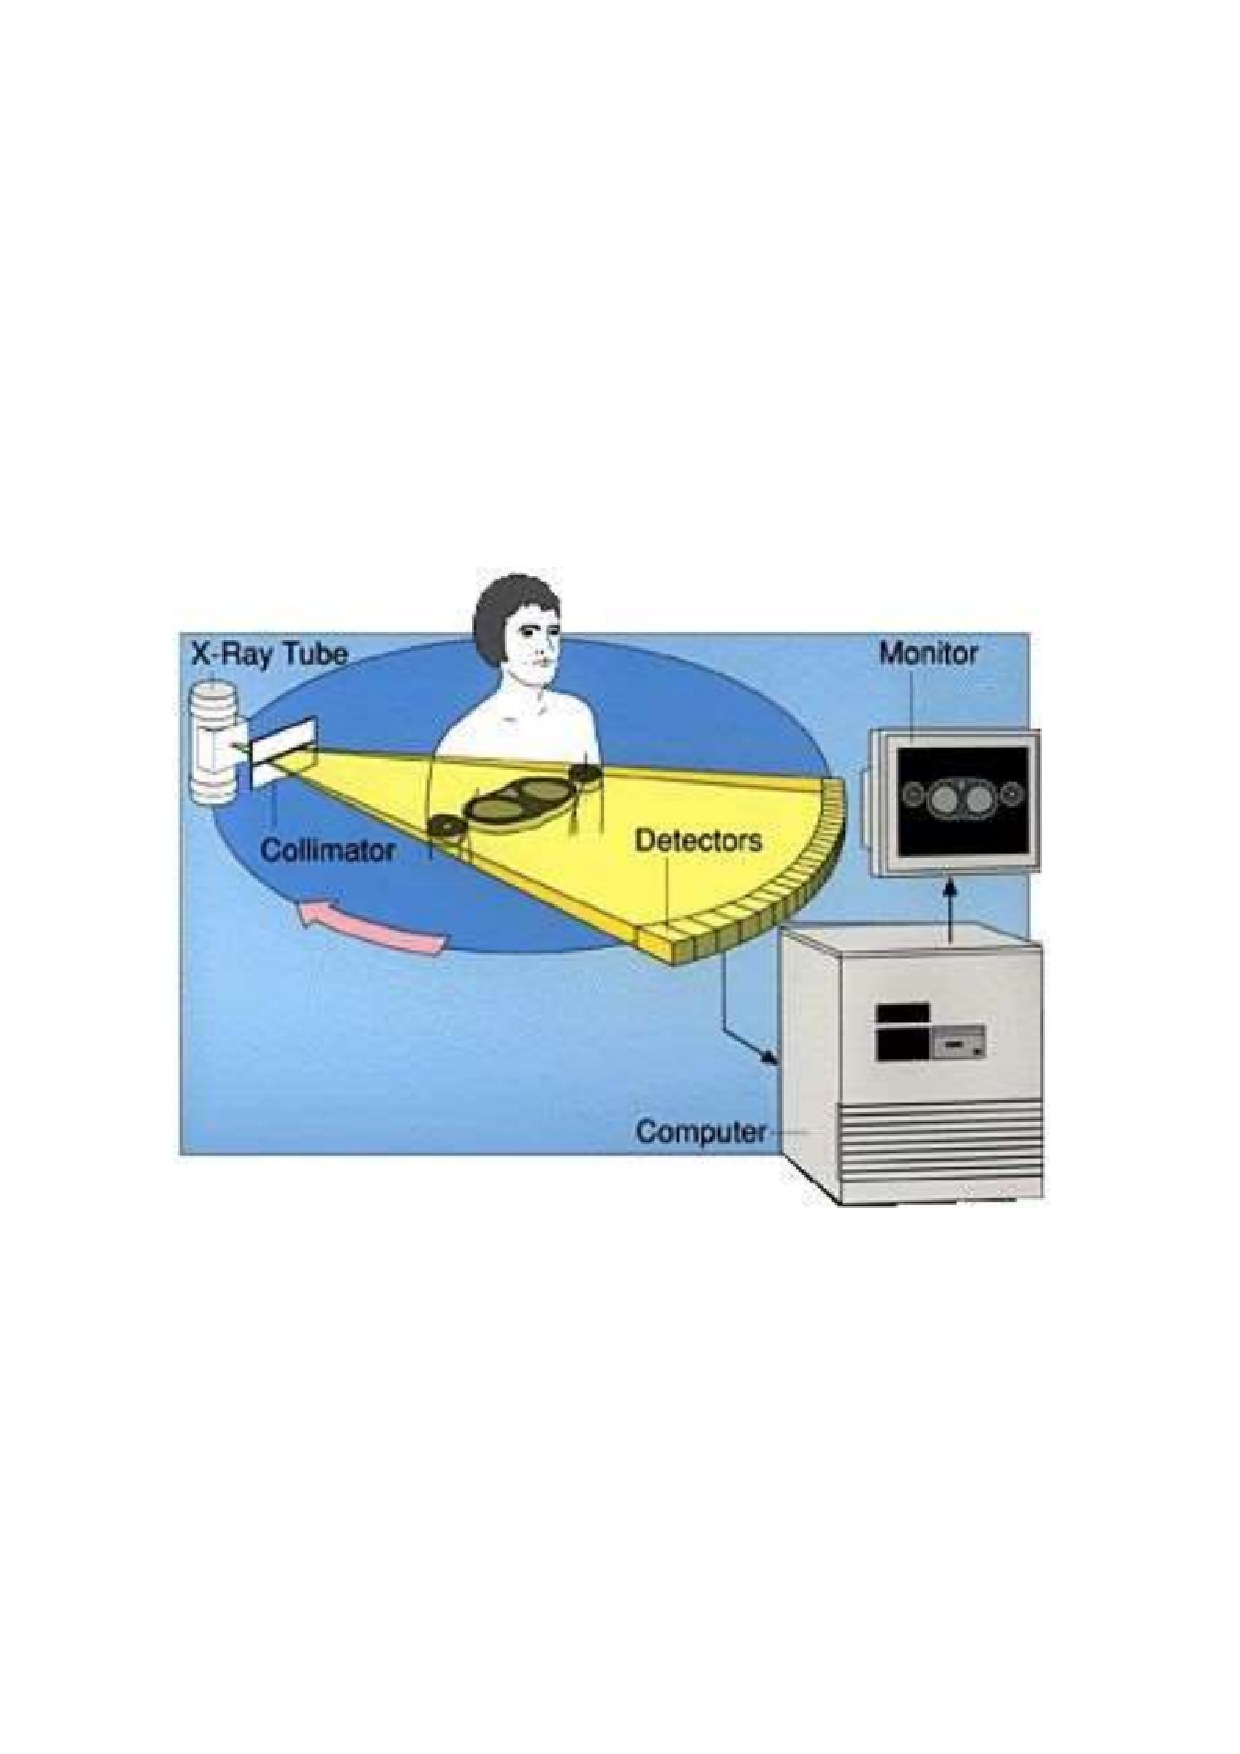
\includegraphics[width=0.5\linewidth,trim={3cm 7cm 3cm 7cm}]{figs/ct_ilustrace.pdf}
    % \caption{}
    % \label{fig:enter-label}
\end{figure}

\newpage
\subsection{PET} 
- metoda založená na pozitron-elektronové anihilaci
- zdroj pozitronů - beta rozpad
\subsubsection{Základní součástky PET tomografu}
\begin{itemize}
    \item gantry, vyšetřovací lúžko, systém detektorů, počítač, laserové zaměřovače
\end{itemize}
- zdroj pozitronů: nejčastěji \iso{18}{F} v deoxyglukóze, 
- detektory - scintilační detektory (NaI(Tl), berylium germaniový, gadolinium-křemíkový, lutecium-křemíkový), počet detektorů udává rozlišení (tisíce)
- princip je podobný jako u CT, pomocí detekovaných fotonů z anihilace je pro daný úhel vytvořena projekce, kompletní projekce tvoří sinogram
- sinogram -> rekonstrukční algoritmus -> finální obraz
\subsection{Rozlišení obrazu}
- co narušuje obraz:
\begin{itemize}
    \item útlum - dáno tloušťkou tkáně, fotoefektem, Comptonovým jevem (sekundární gamma je tlumeno)
    \item Comptonův rozptyl
    \item náhodná koincidence
\end{itemize}

- často mohu kombinovat CT a PET
- z CT získám anatomickou strukturu, z PET biologické procesy


\begin{figure}[ht!]
    \centering
    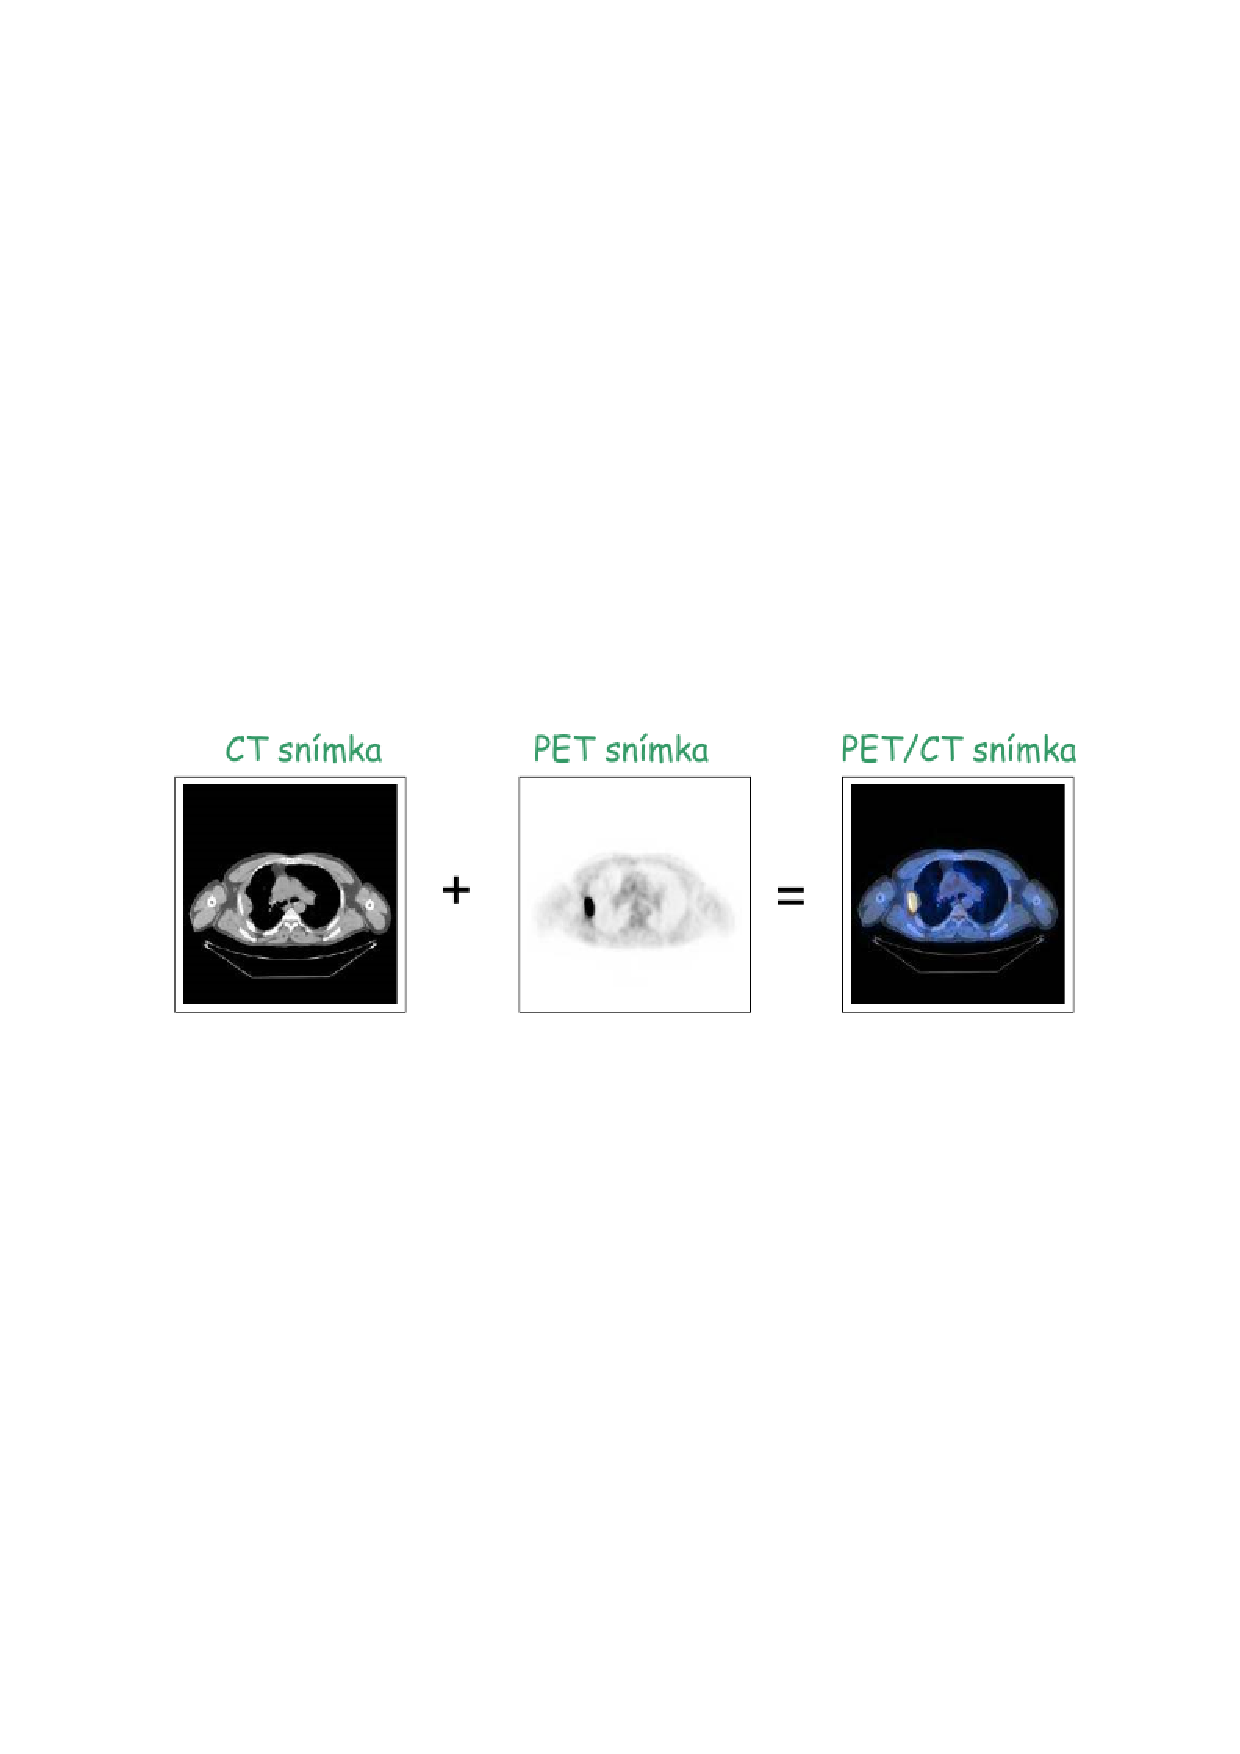
\includegraphics[width=0.8\linewidth, trim={1cm 11cm 1cm 11cm}, clip]{figs/pet_obrazy.pdf}
    \caption{Snímky z CT a PET tomografie}
    \label{fig:2_6_CT_PET_tomografie}
\end{figure}

\newpage
\section{Využití synchrotronového záření v materiálovém výzkumu - získání synchrotronového záření a jeho vlastnosti,
příklady experimentálních technik}

- Synchrotronové záření, někdy také nazývané jako magnetické brzdné záření je záření vysílané relativistickými elektrony kroužícími v magnetickém poli a vzniká tak při pohybu nabité částice se zrychlením. Dochází tak k uvolňování ELMG záření.

- Jelikož je zrychlení vektorové, nemusí docházet ke zpomalování nebo zrychlování nabité částice, ale stačí změna dráhy pohybu a tím se také utváří zrychlení, jež vede na uvolnění části energie do okolí (elmg záření).

- Dále platí, že pokud je při změně dráhy pohybu rychlost částice malá, tak emitované záření je uvolňováno izotropně. Pokud je rychlost vysoká (v/c je cca 1), tak je záření soustředěno do kuželu ve směru pohybu částice s určitým úhlem rozevření kužele, jež závisí na Lorentzovu faktoru, který je nepřímo úměrný rychlosti (čím větší rychlost tím menší rozevření kužele).

\subsection{Schéma uspořádání synchrotronu:}

Sychrotron je cyklický urychlovač částic, jež se skládá z elektronového děla, lineárního urychlovače pro prvotní zrychlení částice a posléze ze dvou prstenců (urychlující a akumulační). Vývodem akumulačního prstence je trasa vedoucí do koncové stanice, kde je realizován experiemnt.

\begin{figure}[ht!]
	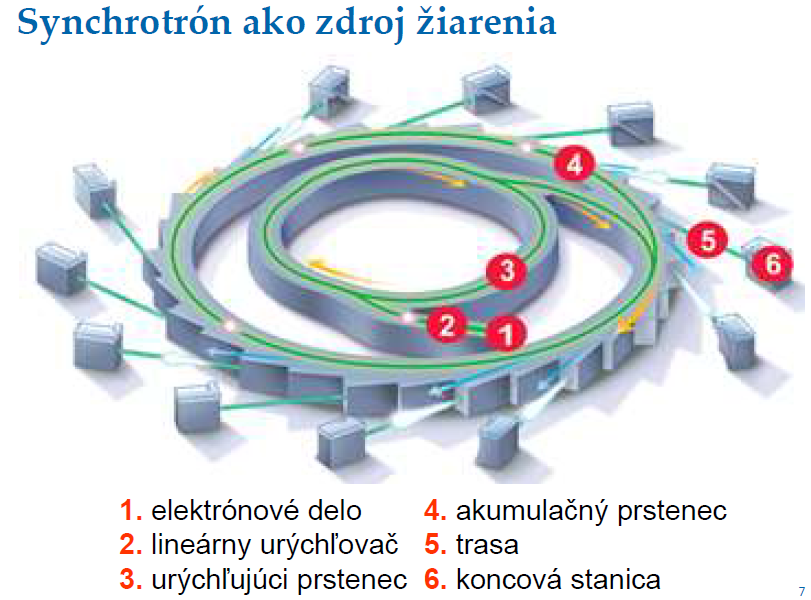
\includegraphics[width=7cm]{synchrotron.png}
	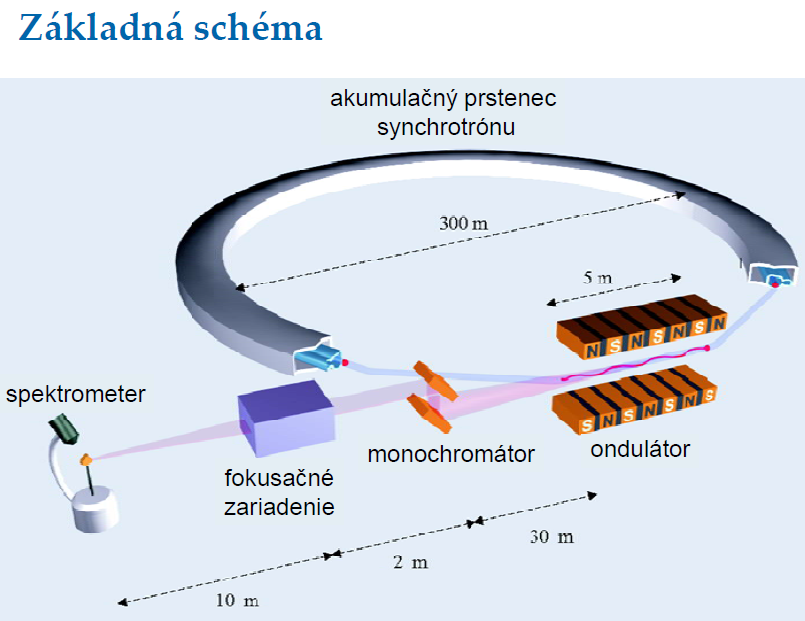
\includegraphics[width=7cm]{synchrotron2.png}
	%	\includegraphics[width=7cm]{rbs3.png}
\end{figure}

\subsection{Tvorba synchrotronového záření}

-Bylo již řečeno v jakých případech a jak vzniká synchrotronové záření, ale jak se to dělá v praxi?

- V praxi se využívá tzv. vlkádacích zařízení, kterými jsou: ohybací magnet, Wigglery a Ondulátory

\begin{itemize}
    \item \underline{Ohybací magnet}: Ohybací magnet slouží k zakřivení dráhy pohybu nabité částice a přitom je tečně k dráze pohybu uvolňováno záření, které se pak dá kolimovat.

    \begin{figure}[ht!]
        \centering
        \includegraphics[width=0.5\linewidth]{ohybací magnet.png}
        \caption{ohybací magnet}
    \end{figure}
    \item \underline{Wiggler}: Zařízení, jež je tvořeno větším počtem dvojic permanentních magnetů, které zapříčiní klikacení dráhy pohybu částice a to způsobuje tvorbu širokého svazku nekoherentního záření. Intenzita záření je úměrná N (počet magnetů).

    \begin{figure}[ht!]
        \centering
        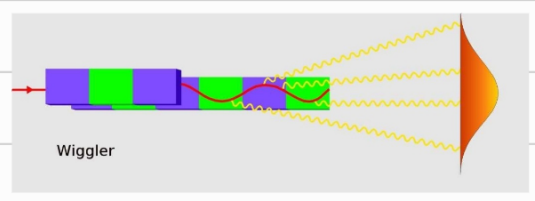
\includegraphics[width=0.5\linewidth]{Wiggler.png}
        \caption{Wiggler}
    \end{figure}
        
    \item \underline{Ondulátor}: Je to to samé co wiggler (opět permanentní magnety), ale magnety jsou slabé a je to asi i delší. Ta částice se tudíž neklikatí tolik a výsledná intenzita emitovaného záření je dokonce úměrná $N^2$, kde N je počet magnetů

    \begin{figure}[ht!]
        \centering
        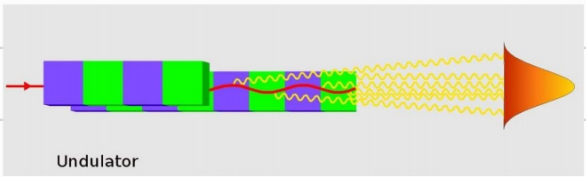
\includegraphics[width=0.5\linewidth]{Ondulátor.png}
        \caption{Ondulátor}
    \end{figure}
    
\end{itemize}


\subsection{Vlastnosti synchrotronového záření}

\begin{itemize}
    \item Spojité a velmi široké spektrum (od IR po RTG záření)
    \item Vysoká monochromatizace
    \item Při využití ondulátorů, je záření koherentní
    \item Stabilita svazku
    \item Impulzní emise (Záření je emitované časticemi a podle počtu částic je to víc spojité a nebo více impulsní.
    \item Přeladitelnost (můžeme si vybrat energii). -> Více stupňová monochromatizace na monokrystalech Si => Monochromátor s vysokým rozlišením (rozptyl cca 1 meV) => kolimace a fokusace pomocí Be čočky nebo K-B zrcadlo a tím fokusace až na rozměry 4x10 $\mu m^2$
    \item Polarizované
    \item Briliance = kombinace toku, velikost zdroje, divergence svazku = jedná se v zásadě o trochu komplikovanější Intenzitu pro popis elektromagnetického záření. 
\end{itemize}


\underline{Využití:}

- Dá se využít pro jaderný rezonanční rozptyl (studium hyperjemných interakcí, vibrační vlastnosti jader, magnetické přechody apod. a to za extrémních vnějších podmínek = magnetické pole, kryo, vysoká teplota apod..)

- RTG mikroskopie - využití RTG svazků s rozlišením v řádu desítek nm a zobrazení tenkých vrstev a povrchů.

- Transmisní X-ray mikroskopie (TXM) - Dobrý kontrast, vysoké rozlišení

- RTG sepktroskopie = měření chemického složení.

- RTG absorpční spektroskopie = informace o typu a vzdálenostech sousedních atomů

- RTG tomografie = 3D obrazy drobných objektů s velmi vysokým rozlišením na úrovni mikrometrů.ě
\\

\underline{XFEL:} 

- Zařízení XFEL (X-Ray Free Electron Laser) je zařízení, které je v podobě lineárního urychlovače (European XFEL) a umožňuje lineárně urychlovat elektrony až na energie 17 GeV. Urychlené elektrony pak projdou ondulátorem a vzníká záření jako ze synchrotronu, které má rozsah energií od 0,01 - 20 keV (velmi malá vlnová délka).

- Velmi malá krátkost pulsů (cca desítky fs)

- o 10 řádů vyšší briliance jako u 3. generace sychrotronů. 

- V zásadě jsou dány frekvence na balík (jak často přichází balík elektronů, resp. pulsu), ale pak je ještě samotná frekvence v rámci balíku a proto je krátkost pulsů velmi malá.

\begin{figure}[ht!]
    \centering
    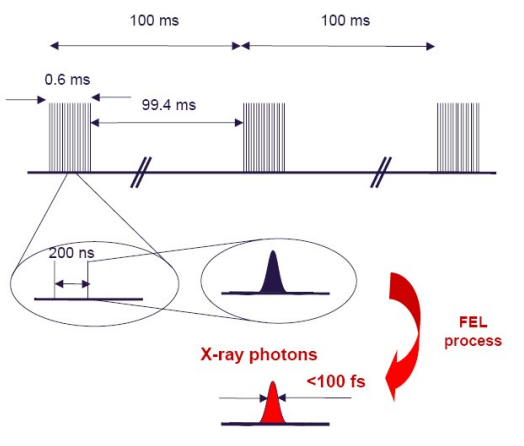
\includegraphics[width=0.5\linewidth]{časová struktura pulsů fotonů.png}
    \caption{časová struktura pulsů fotonů}
\end{figure}

\newpage
\section{Jednotky a veličiny v dozimetrii, základy legání metrologie, etalony a stanovená měřidla}

Metrologie je věda zabývající se měřením a mezi základní cíle a úkoly patří:
\begin{itemize}
    \item definice jednotek a jejich realizace pomocí vědeckých metod
    \item vývoj a udržování etalonů nejvyšší úrovně
    \item zajištění fungování měřidel ve výrobní sféře
    \item zajistit správnost měření v úředních nebo obchodních sférách
\end{itemize}

\subsection{Základy legální metrologie}

-Hlavním je zákon č. 505/1990 Sb. o metrologii => upravuje práva a povinnosti subjektů a státních orgánů správy pro účely zajištění správnosti a jednotnosti měřidel a měření
\\

- Dále jsou důležité prováděcí vyhlášky k samotnému zákonu, a to sice:
\begin{itemize}
    \item Vyhláška MPO č. 262/2000 Sb., kterou je zajišťována jednotnost a správnost měřidel a měření

    \item Vyhláška MPO č. 345/2002 Sb., kterou se stanoví měřidla k povinnému ověřování a měřidla podléhající schvalování

    \item Vyhláška MPO č. 264/2000 Sb., o základních měřících jednotkách a ostatních jednotkách a o jejich označování
\end{itemize}

\underline{Klasifikace měřidel:}
\begin{itemize}
    \item Etalony (primární, sekundární, mezinárodní, státní) = objekt či něco jiného, jež obecně slouží k uchování a realizaci dané jednotky (etalon hmotnosti, kde jednotka je kg, tak je snad krystal křemíku, protože umíme přesně určit počet atomů v mřížce).
    \item Stanovená měřidla = Jedná se o měřidla, která MPO (ministerstvo průmyslu a obchodu) vyhláškou stanoví k povinnému ověřování s ohledem na jejich význam (obchod, daně, sankce, tarify, poplatky, medicína, ochrana ŽP, BOZP).
    \item Pracovní měřidla = jedná se o měřidla jež nejsou etalonem ani stanoveným měřidlem
    \item Certifikované a ostatní referenční materiály = Jedná se o materiály přesně stanoveného a známého chemického složení, které slouží pro ověřování nebo ke kalibraci (často to bývají etalony)
\end{itemize}

- Schvalování typů měřidel je proces, při kterém jsou ověřeny metrologické a technické vlastnosti stanovených měřidel, jež vycházejí z technických norem.
Zkoušky pro schválení typu stanoveného měřidla obsahuji funkční zkoušky, zkoušky odolnosti proti rušivým vlivům vnějšího prostředí a zkoušky elektromagnetické kompatibility. Výsledkem je certifikát a přidělení značky schválení typu.
\\

- Pod pojmem návaznost rozumíme: (definice je na hovno) V zásadě se jedná o to, že vemu např. 8 vah z celého světa, nastavím je pomocí kvalitního etalonu na to, že toto je 1kg a potom, když něco naměřím já, tak i Karlíkovi z horní dolní můžu věřit, že to má jak já, protože to má nastavený v návaznosti na ten samý etalon a tudíž i v návaznosti na mne.
\\

- Ověřování je proces, resp. potvrzení, že měřidlo má požadované metrologické vlastnosti.
\\

- Kalibrace je proces, kdy je periodicky upravováno a kontrolováno, že měřidlo měří to co má a případná kalibrace probíhá pomocí certifikovaných a ostatních referenčních materiálu, kterými jsou nejčastěji etalony.
\\

\underline{ÚNMZ = Ústav pro technickou normalizaci, metrologii a státní zkušebnictví}

- Zastupování ČR ve věci mezinárodních věcí s ohledem na metrologii

- Dohled na činnosti ČMI

- Kontrola dodržování zákona o metrologii

- Schválení a vyhlášení státních etalonů

- Poskytování metrologických expertíz
\\

\underline{ČMI}

- Uchovávání a rozvoj státních etalonů

- Schvalování typů a ověřování stanovených měřidel

- Certifikace referenčních materiálů

- Kalibrační služby
\\

\subsection{Veličiny a jednotky - legislativa}

Existují různé soustavy jednotek, kde nejvíce je rozšířené SI, dále existuje imperiální, americká apod... Stačí znát SI

- V obecnosti jsou základní jednotky SI popsáné v Zákoně č. 505/1999 Sb. o metrologii. Obsaženy jsou dále odvozené jednotky, násobky, díky a jiné povolené jednotky.
\\

Základní jednotky a veličiny SI jsou:
\begin{itemize}
    \item Čas - s
    \item Proud - A
    \item Svítivost - cd
    \item Látkové množství - mol
    \item Teplota - K
    \item Hmotnost - kg
    \item Délka - m
\end{itemize}

- Odvozené jednotky vyjadřované jednotkami základními jsou např. hustota, objem, plocha, rychlost,...

- Odvozené jednotky se zvláštním označením i názvem jsou např. náboj, síla, aktivita, absorbovaná dávka,...

- Odvozené jednotky vyjádřené jednotkami základními spolu s jednotkami se zvláštním názvem a označením jsou např. Expozice, PDE, dávkový příkon, dávkový ekvivalent,...
\\

\underline{Vlastnosti a výhody SI:}
\begin{itemize}
    \item Systematická a mezinárodně uznávaná soustava veličin a jednotek
    \item Pro každou veličinu zavedena pouze jedna jednotka
    \item Odvozené jednotky tvořeny součiny mocnin základních jednotek
    \item Násobky a díly jednotek vyjádřeny předponami
\end{itemize}


\underline{Další mimosoustavné jednotky} - jsou použitelné spolu s SI v rámci specifikovaných oborů a nebo výjimečně a tehdy, jeli definován vztah k SI jednotkám.
\begin{itemize}
    \item Uzel
    \item dioptrie
    \item Angstrom
    \item barn
    \item 1 atm
    \item curie
    \item calorie
\end{itemize}


\underline{Veličiny ve vztahu k atomové a jaderné fyzice:}

- Aktivita, přeměnová konstanta, poločas rozpadu, barn, hustota toku, fluence, absorbovaná dávka, kerma, expozice, dávkový ekvivalent, efektivní dávka, PDE,...

\subsection{Jednotky a veličiny v dozimetrii}

\underline{Expozice:}

- Definována pro popis ionizujících účinků fotonů ve vzduchu [X] = C$\cdot kg^{-1}$.

- Expozice je definována jako podíl celkového náboje dQ iontů jednoho znaménka, jež vznikly při úplném zabrzdění všech elektronů a pozitronů uvolněných fotony v malém objemu vzduchu, a hmotnosti tohoto objemu vzduchu dm.

\begin{center}
    \begin{equation}
        X = \frac{dQ}{dm}
    \end{equation}
\end{center}

\begin{figure}[ht!]
    \centering
    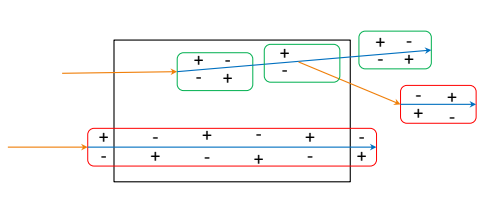
\includegraphics[width=0.5\linewidth]{expozice.png}
    \caption{expozice}
\end{figure}

\underline{Absorbovaná dávka}

- Vyjadřuje střední energii předanou IZ dané látce o jednotkové hmotnosti

- Jednotkou absorbované dávky je [D] = Gy

\begin{center}
    \begin{equation}
        D = \frac{\overline{\varepsilon}}{dm}
    \end{equation}
\end{center}

\underline{Kerma}

- Popisuje působení nepřímo ionizujícího záření z hlediska energetických ztrát primárních částic

- Jednotkou Kerma je: [K] = Gy


\begin{center}
    \begin{equation}
        K = \frac{dE_k}{dm}
    \end{equation}
\end{center}

\underline{Dávkový ekvivalent, resp. ekvivalentní dávka}

- Jedná se o veličinu jž využívá tzv. faktoru kvality Q, kterým je přenásobena absrobovaná dávka a tento faktor kvality pak popisuje vliv daného IZ na tkáň (bez rozdělování o jakou tkáň se jedná).

- Q=1 pro elektrony, gama a RTG, dále je Q=10 pro protony, neutrony a Q=20 pro nabité ionty, alfa částice, štěpné produkty

\begin{center}
\begin{equation}
    H = Q \cdot D
\end{equation}    
\end{center}


\underline{Efektivní dávka}

- Jedná se o Dávkový ekvivalent násobený dalším faktorem kvality, a to tentokrát tkáňovým faktorem, který zohledňuje ještě dále, jaká část těla schytala to záření, protože každá část těla je jinak náchylná/odolná. To v praxi znamená, že kostní dřeň je snad nejvíce náchylná, zatímco játra nebo oko, dlaň (kůže) není tolik.

\begin{center}
    \begin{equation}
        D \cdot w_r = H, E = \sum_T w_T \cdot H_T
    \end{equation}
\end{center}

\newpage
\section{Využití proporcionálních detektorů a kapalných scintilátorů v metrologii aktivity radionuklidů}

-Metrologie radioaktivity radionuklidů je dělena do dvou základních skupin:

\begin{itemize}
    \item Absolutní = Využívá přímé detekce veličiny (Koincidenční metoda, elektrostatická metoda, kalorimetrická metoda, absolutní počítání částic).
    \item Relativní = Vztah mezi veličinou indikovanou a veličinou měřenou (spektrometrie gama, ionizační komora)
\end{itemize}

\subsection{Využití proporcionálních detektorů}

- Jedná se o primární metodu měření = vychází z definice veličiny.

- Proporcionální detektor, je často válcové geometrie a skládá se z anody (tenký drátek z W, Mo, Cu, ocel, Au pokrytí) a katody (tělo detektoru). Díky velkému rozdílu ve velikosti elektrod je mezi nimi velký rozdíl napětí, a to vytváří velmi intenzivní elektrické pole. Pracovním plynem uvnitř detektoru je často Ar, Kr, Xe + zhášecí plyn, což je například Metan nebo propanbutan.

- Výstupní impuls na detektoru je úměrný deponované energii

- Typická náplň je plyn P-10 (90\% Ar a 10\% CH$_4$)

- Důležité je, aby anodový drátek měl konst. průměr a tloušťku

- Výhodou proporcionálního detektoru je, že téměř nemá mrtvou dobu a je tedy hodně dobře schopen detekovat dva signály "naráz"

- Je provozován v oblasti proporcionality VA charakteristiky plynového detektoru, kdy měřená četnost téměř nezávisí na napětí (pracovní napětí detektoru je zvoleno v této oblasti). Provoz v této oblasti umožňuje rozvoj townsendovy laviny, jež představuje plynové zesílení.

- Plynová naplň v detektoru je přítomna za účelem zesílení vstupního signálu = plynové zesílení. Proto je proporcionální počítač vhodný pro detekci záření malých energií, které je pak třeba zesílit právě přítomným plynem (ionizace plynu k zesílení vstupního signálu, a to řádové E2 až E3).

- Proporcionální počítač se používá k měření $\alpha$ a $\beta$ záření.

- Proporcionální počítače lze využít jako prosté detektory čítání, ale také částečně pro spektrometrii/spektroskopii neboť výstupní signál je úměrný vstupnímu, resp. deponované energii (s uvážením zesílení od plynu).
\\

\underline{Druhy proporcionálních počítačů:}
\begin{itemize}
    \item Průtokový: 
        \begin{itemize}
            \item Pracovní plyn protéká detektorem o atmosférickém tlaku a díky tomu je snadná výměna vzorků.
            \item Měření $\alpha$ a $\beta$ záření, zejména pak $\beta$.
            \item Lze udělat i 4$\pi$ variantu
            \item Vhodný pro měření nízkoenergetické $\beta$ a plynných radioaktivních sloučenin i neutronů (pro neutrony je potřeba konverzní materiál).
        \end{itemize}
    
    \item Tlakový: 
    \begin{itemize}
            \item Plynová náplň má vyšší hmotnostní číslo a plyn je natlakován do cca 1,5 MPa.
            \item Vyšší tlak umožňuje dosáhnout vyšší účinnosti detekce záření (Tím, že je to natlakované, tak se tam vejde více plynu a tím se mi zvyšuje pravděpodobnost interakce záření s plynem).
        \end{itemize}
    
\end{itemize}


\underline{Korekce:} - zejména pro interní proporcionální poćítač, kdy je měřený vzorek uvnitř.
\begin{itemize}
    \item Koncový efekt = Na okrajích elektrod je elektrické pole deformované. Lze kompenzovat využitím dvou počítačů různé délky a rozdíl odezvy odpovídá četnosti naměřené ideálním detektorem o délce rozdílu jejich délek.
    \item Stěnový efekt = částice emitovaná v blízkosti stěn nestačí dostatečně ionizovat (oprava na základě
měření s několika počítači stejné délky různých poloměrů, vliv klesá s rostoucím tlakem plynové náplně)
\end{itemize}


\subsection{Využití kapalných scintilátorů}

- Jedná se o scintilační detektor, kde scintilační látka je tekutá/roztok

- Jedná se o roztoky scintilačních látek v organických rozpouštědlech + měřený vzorek, který je v tomto taktéž rozpuštěn (podle druhu měřeného vzorku se používají rozpouštědla jako je toulen, xylen, ethalon

- Kapalné scintilátory se používají pro detekci IZ ($\alpha$ a $\beta$) o vyšších energiích (minimální detekovatelná energie je 3-10 keV).

- Využívají se pro tzv. metodu TDCR (triple to double coincidence ratio)

- Detekční účinnost je dána účinnosti fotokatody daného fotonásobiče (kvalita fotonásobiče)

\subsubsection{TDCR}

- Jedná se o koincidenční zapojení tří fotonásobičů, jež funguje na principu poměru trojných a dvojných koincidencí.

- Tato metoda slouží ke stanovení počítací účinnosti, a to experimentálně bez potřeby kalibračního standardu.

- počítací účinnost ($\varepsilon_D$), neboli parametr TDCR (v zásadě detekční účinnost) se určuje na základě srovnání experimentu a modelu => V praxi je měřeno TDCR pro různé účinnosti detekce, které mohu měnit defokusací PMT, optickými filtry atd. 

Tím získávám závislost naměřené aktivity na TDCR (aktivita by měla být nezávislá na TDCR - kritérium správnosti) a dále závislost detekční účinnosti na TDCR (tu detekční účinnost si měním). Ve výsledku srovnáním experimentu a modelu získám účinnost $\varepsilon_D$.

$\left(\frac{\varepsilon_T}{\varepsilon_D}\right)_{výpočet} = \left(\frac{N_T}{N_D}\right)_{měření}$

- Výsledný počet řešení TDCR parametru se odvíjí od druhu radionuklidu a složitosti jeho kaskády rozpadu).

Výsledná aktivita je získána jako: $A = \frac{N_D}{\varepsilon_D}$

\begin{figure}[ht!]
    \centering
    \includegraphics[width=1\linewidth]{TDCR.png}
    \caption{TDCR}
\end{figure}

\newpage
\section{Koincidenční metoda stanovení aktivity a spektrometrie záření gama jako sekundární metoda měření aktivity}

\subsection{Koincidenční metoda}


- Využívá se faktu, že při RA přeměně RN dochází často k emisi vícero záření/částic.

- V praxi se jedná o využití dvou detektorů, kdy každý je citlivý na jiný druh záření a výstup, resp. impuls na výstupu čítače koincidencí je jen v případě, když dojde k "současnému" výskytu impulsů na obou detektorech (vstup A i B). Je nutné, aby impulsy byly zaznamenány v rámci tzv. rozlišovací doby. V opačném případě není zaznamenána koincidence, ale pouze výstup na čítači A či B.

\begin{figure}[ht!]
\centering

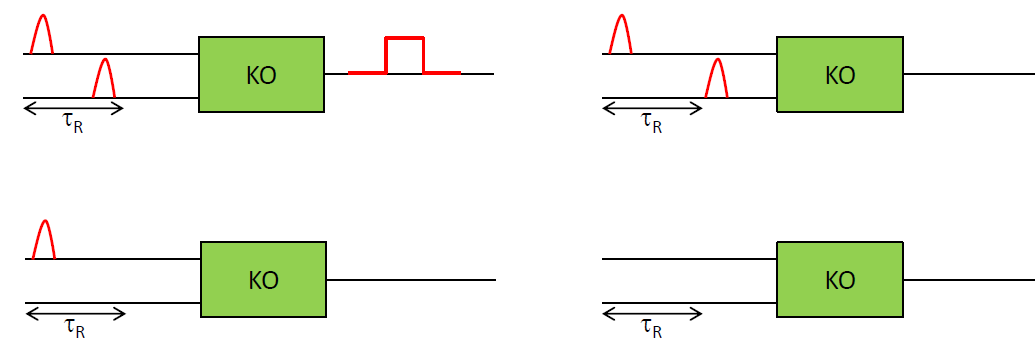
\includegraphics[width=0.7\linewidth]{koin-obvod.png}
%	\includegraphics[width=7cm]{prutok-propor.png}
	%	\includegraphics[width=7cm]{rbs3.png}
\end{figure}

\begin{figure}[ht!]
    \centering
    \includegraphics[width=\linewidth]{jednoduché koincidenční zapojení.png}
    \caption{jednoduché koincidenční zapojení}
\end{figure}

\underline{Rozlišovací doba} může být stanovena dvěma způsoby, a to:
\begin{itemize}
    \item Generátor - Pomocí generátoru si mohu nastavovat časový interval mezi generovanými signály a měřit jak citlivý je detekční systém na různé časové intervaly. Postupně se mění rozlišovací doba a sleduje se, kdy systém správně detekuje koincidenci.
    \item Náhodné koincidence - Postupně se snižuje rozlišovací doba a měří se náhodné koincidence. Jakmile začne počet zaznamenáných koincidencí výrazně klesat, začiná se přibližovat optimální rozlišovací době. Cílem je najít takovou rozlišovací dobu, která minimalizuje počet náhodných koincidencí zatímco stále zachovává koincidence, které chci měřit.
\end{itemize}

Důležité je však znovu zdůraznit, že do celkového počtu koincidencí se mi projeví jak pravé tak náhodné koincidence a proto je žádoucí nastavit rozlišovací dobu správné.


\begin{figure}[ht!]
    \centering
    \includegraphics[width=1\linewidth]{Výsledné zapojení koincidenčního obvodu.png}
    \caption{Výsledné zapojení koincidenčního obvodu}
\end{figure}

Dobré vědět k čemu slouží jednotlivé komponenty:

\begin{itemize}
    \item Detektor = záznam/detekce signálu od IZ.
    \item Předzesilovač = Jeho hlavním úkolem je zesílit slabé signály z detektoru na úroveň, která je dostatečná pro další zpracování. Důležité je, aby zesílení proběhlo bez výrazného zvýšení šumu (změnou nastavení impedance), což by mohlo negativně ovlivnit kvalitu signálu. Další úlohou je přivedení pracovního napětí na detektor.
    \item Zesilovač = zvyšuje úroveň signálu, který již byl zesílen předzesilovačem, na úroveň vhodnou pro zpracování dalšími elektronickými obvody, jako je například jednokanálový analyzátor. Musí poskytnout stabilní a lineární zesílení signálu, aby nedocházelo k deformaci (zkreslení) původního signálu
    \item Zpožďovací linka = záměrně zpožďuje signál přicházející z detektoru o určitou dobu. Její hlavní funkcí v koincidenčním měření je zajistit, aby signály z různých detektorů dorazily do koincidenčního obvodu ve správném časovém rozmezí, i když mají různé dráhy nebo rychlosti zpracování. To je důležité pro správnou identifikaci koincidenčních událostí, protože signály musí dorazit téměř současně, aby byly považovány za koincidentní.
    \item JKA = Jednokanálový analyzátor slouží k selekci signálů podle jejich amplitudy, což odpovídá energii detekovaného záření. Signál má tak posléze formu 1 nebo 0, tedy splňuje nebo nesplňuje. Propustí pouze ty signály, jejichž amplituda spadá do definovaného rozsahu (dolní hranice stanovená diskriminací).
    \item Obvod mrtvé doby = Obvod mrtvé doby je navržen tak, aby po detekci jednoho signálu zablokoval možnost detekce dalších signálů po určitou dobu. Mrtvá doba je důležitá pro zabránění registrace falešných koincidenčních událostí způsobených příliš blízkými nebo souběžnými událostmi, které by mohly být mylně považovány za koincidentní.
    \item Koincidenční obvod
    \item Čítač
\end{itemize}

\subsubsection{Instrumentální opravy}

\begin{itemize}
    \item korekce na pozadí, náhodné koincidence a mrtvou dobu 


    \item aplikace koincidenční metody: 
    \begin{itemize}
        \item 4$\pi \, \beta - \gamma$: nuklidy \iso{24}{Na}, \iso{42}{K}, \iso{56}{Co}, \iso{59}{Fe} => při této koincidenční metodě je RN vložen do interního počítače (měření $\beta$) a okolo počítače jsou např. scintilační detektory pro měření $\gamma$. Celé je to posléze stíněné pro minimalizaci vlivu pozadí.
        
        \item 4$\pi \, \alpha - \gamma$: \iso{210}{Po}, \iso{241}{Am}

        
    \end{itemize}
\end{itemize}
\subsubsection{Korekce - Opravy jednoduchého jaderného schématu}
\begin{itemize}
    \item vnitřní konverze - vyzáření elektronu z obalu (konverzní elektron) a u toho vzniká ještě doprovodné charakteristické RTG záření => detekce KE v $\beta $ kanálu. Není to to samé jako Beta přeměna. Jedná se o konkurenční proces k emisi fotonu při deexcitaci. Oprava probíhá úpravou vztahu pro výpočet elektronů v $\beta$ kanálu, tedy poměr naměřených četností/aktivita. 
    \item citlivost kanálu $\beta$ na záření $\gamma$ řeším úpravou koincidenční rovnice. V opačném případě, kdy jsou elektrony v $\gamma$ kanálu, lze využít například stínění detektorů, kterým částice Beta neprojde.
    \item brzdné záření - většinou zanedbatelně malý vliv, ale dělá to vliv záření $\beta$ na detektor citlivý na $\gamma$. Pokud chceme, tak se opět mohou dělat opravy koincidenční rovnice. Možná by se toho šlo zbavit vhodným nastavením diskriminace?
    
\end{itemize}

\subsubsection{Metody}
\begin{itemize}
    \item \textbf{extrapolační metoda} -Spočívá v uskutečnění série měření pro různé hodnoty detekční účinnosti v kanále $\beta$ ($\varepsilon_\beta = \frac{n_k}{n_\gamma}$), čehož docílíme např. překrytím vzorku filmem či změnou diskriminace/zesílením (upravuji účinnost v kanále $\beta$). Výsledná závislost (účinnost na $\frac{n_\beta \cdot n_\gamma}{n_{PK}}$ ) (viz rovnice níže) je lineárně proložena a extrapolována k nule (s -> 0). Všechny výše zmíněné opravy lze uvažovat ve společném tvaru $$M = \dfrac{n_{\beta} n_{\gamma}}{n_{PK}} = A \cdot [1 + S\cdot k] $$ \\
   \item Stopovací metoda: přimíchám čistý ZIZ $\beta$ se vzorkem $\beta-\gamma$, použiju přincip extrapolační metody (získám měření pro různé poměry aktivity vzorku a celku). V praxi funguje tak, že smíchám čistý zdroj IZ $\beta$ a vhodný radionuklid s kaskádou $\beta - \gamma$. Posléze měřím celkovou aktivitu směsi ($A_{xs}$) a aktivitu RN s kaskádou ($A_s$). Odečtením jednoho od druhého dostanu aktivitu čistého zdroje IZ $\beta$ ($A_x$) => $A_{xs} = A_x + A_s$.
    \item záchytové radionuklidy - měřím koincidenci záření X$_{\text{K}}$ a X$_{\text{L}}$ - čistý záchyt elektronu
    \item záchytové radionuklidy - měřím koincidenci záření X - $\gamma$ - obdoba kaskádám $\alpha - \gamma$, větší uplatnění korekčních faktorů, oboje měření se záchytovými radionuklidy je těžší na provedení, neboť si zde konkurují různé proces
    
    \end{itemize}

\subsection{Spektrometrie gama jako sekundární metoda měření aktivity}

\underline{Interakce fotonů s látkou:}

\begin{itemize}
    \item Fotoelektrický jev (energie fotonů je zpravidla nejmenší) - energie je všechna předána elektronu a dochází k jeho vyražení z elektronového obalu. Jeho prázdné místo je zabráno elektronem z vyšší energetické hladiny/slupky a rozdíl energií je vyzářen v podobě RTG charakteristického záření.

    \item Comptonův rozptyl: (vyšší energie gama fotonů) - Část energie je předána elektronů a dochází k jeho vyražení. Platí, že fotoefekt je závislý na hmotnostním čísle, ale Comptonův jev není, a proto je pro lehká jádra pravděpodobnější Comptonův rozptyl.

    \item Tvorba elektron-positronového páru: Energie iniciujícího fotonu musí být vyšší než je 1,02 MeV (2x511 keV) a ideálně o něco vyšší. Dochází k přeměně fotonu v blízkosti jádra atomu na pár elektron a positron. Přebytek energie je předán jádru v podobě hybnosti. Při jejich zániku rekombinací vzniká tzv. anihilační fotony, které mají 2x$\gamma$ pod úhlem 180$^\circ$ o velikosti 2x511 keV. Tato energie je tam dána jako podmínka, protože klidová energie, resp. hmotnost elektronu i positronu je 511 keV.
\end{itemize}


\underline{Spektrometrická trasa:}

\begin{figure}[ht!]
\centering
	\includegraphics[width=0.8\linewidth]{spek-trasa.png}
	%	\includegraphics[width=8cm]{elektorstaticka-metoda2.png}
	%	\includegraphics[width=7cm]{rbs3.png}
\end{figure}

MCA = Mnohokanálový analyzátor - počítá impulzy z detektoru v závislosti na velikosti jejich amplitudy. Umožňuje nastavovat počet kanálů (jejich šířka energií), diskriminace, oprava na mrtvou dobu, zesílení,..
\\

\underline{Detektory pro spektrometrii gamma}: Jedná se o materiály s vysokým protonovým číslem
\begin{itemize}
    \item Scintilační detektory = NaI(Tl), LaBr$_3$(Ce), CsI(Tl) => Mají vyšší účinnost a nemusí být chlazeny (možný provoz za pokojové teploty).
    \item Polovodičové detektory = Vysoké energetické rozlišení, ale nutno při provozu chladit na teplotu kapalného dusíku. (HPGe, Si(Li)).
    \item Je dobré mít zajištěné vhodné stínění, na čež se používají materiály s vysokým hmotnostním číslem a také vícevrstvé řešení (Pb, Cd, Cu).
\end{itemize}


\underline{Spektrum detektorů různých velikostí:}
\begin{itemize}
    \item Malé detektory = rozměr je menší než střední volná dráha rozptýleného fotonového záření. Spektrum je tak tvořeno Comptonovým kontinuem, DEP a píkem úplné absorpce.

\begin{figure}[ht!]
    \centering
    \includegraphics[width=0.75\linewidth]{male detektory spektrum.png}
    \caption{male detektory spektrum}
\end{figure}
    
    \item Středně velké detekotry = rozměr je srovnatelný se střední volnou dráhou, a proto spektrum obsahuje to samé co pro malé detektory, ale dále navíc SEP a část spektra náležící vícenásobnému rozptylu.

\begin{figure}[ht!]
    \centering
    \includegraphics[width=0.75\linewidth]{Středně velké detekotry spektrum.png}
    \caption{Středně velké detekotry spektrum}
\end{figure}
    
    \item Velké detektory = Všechny události přispívají do píku úplné absorpce.

\begin{figure}[ht!]
    \centering
    \includegraphics[width=0.75\linewidth]{Velké detektory spektrum.png}
    \caption{Velké detektory spektrum}
\end{figure}
    
\end{itemize}

\underline{Spektrometrické stanovení aktivity:}

- Stanovení aktivity na základě plochy píku, píkové účinnosti, radiačního výtěžku a živé doby měření. 

- Deteční účinnost se pak ještě dělí na absolutní, vnitřní, celkovou a píkovou, kde detekční účinnost obecně znamená podíl počtu částic, které jsou zaznamenány a počet částic emitovaných zdrojem. Píková detekční účinnost obsahuje pouze interakce, jenž patří do píku úplné absorpce.

\begin{center}
    \begin{equation}
        A = \frac{P}{\varepsilon Y t}
    \end{equation}
\end{center}
















\newpage
\section{Metrologie neutronů a metoda manganové lázně včetně zpracování výsledků měření a zdrojů chyb a nejistot.}

- Z hlediska metrologie neutronů je dobré zmínit nejprve veličiny jako je hustota toku neutronů ($\phi$), neutronová fluence ($\varphi$) nebo emise radionuklidového zdroje neutronů (S).
\\
\underline{Hustota toku neutronů $\phi$} = to samé co fluence, ale za 1s.
\underline{Neutronová fluence $\varphi$} = podíl počtu neutronů jež dopadnou z libovolného směru na malou kouli a plochy jejího příčného průřezu (kolik neutronů mi projde plochou celkově za celý čas měření)

\underline{Emise} zdroje $S$ (s$^{-1}$)= počet částic emitovaných ze zdroje za jednotku času.



\subsection{Zdroje neutronů}

\underline{Radionuklidové zdroje}
\begin{itemize}
    \item ($\alpha$, n), ($\gamma$, n), spontání štépení
    \item ($\alpha$, n) = typicky AmBe s emisí od $10^5 - 10^8$ za sekundu a energií neutronů od 5 do 10 MeV. Dále existuje PuBe
    \item ($\gamma$, n) = SbBe, NaBe nebo $D_2O$. Výhodou tohoto typu zdrojů je produkce takřka monoenergetických neutronů, avšak za cenu nižší energie.
    \item spontání štépení = v praxi se využívá hlavně a snad jen 252-Cf, jež má cca 3\% pravděpodobnost spontáního štěpení a zbytek je alfa přeměna.
    \item Mezi hlavní výhody patří relativně nízká cena, dostuponost, transport, malé rozměry, nízké nároky na provoz a údržbu
    \item Nevýhodou je neproměnné spektrum, nižší emise neutronů, doprovodné gama záření a nemožnost vypnutí zdroje.
\end{itemize}

\underline{Generátory neutronů:}

- Využívájí fůzních reakcí ve formě D-D, D-T či T-T reakcí za vzniku 3-He, 4-He a 4-He. Největší energie reakce je při fúzi D-T. V zásadě se jedná o zásobník s plynem částic, které jsou pak urychlovací trubicí (jak urychlovač) urychlovány a dopadají na terčík.

\subsection{Metoda manganové lážně}

- Jedná se o metodu pro standardizaci emise $S$ zdrojů neutronů.
\\

\underline{Princip}
\begin{itemize}
    \item Aktivace 55-Mn ve vodném roztoku $MnSO_4$ pomocí neutronů za vzniku 56-Mn
    \item Rozpad 56-Mn s poločasem rozpadu cca 2,5h na železo 56-Fe, elektron a gama.
    \item Mangan se využívá, neboť má vysoký účinný průřez pro absorpci neutronů (tepelné neutrony cca 100 barnů).
    \item Emise neutronového zdroje $S$ je stanovena na základě saturované aktivity 56-Mn, avšak se zohledněním absorpce neutronů na kyslíku, síře, vodíku a dále se musí zohlednit vliv prahových reakcí na jádrech síry a kyslíku ($T$), korekce na neutrony ztracené ve zdroji a dutinách ($C$) a na závěr korekce na únik neutronů z lázně ($L$).
    \item Saturované aktivity je dosaženo po cca 10 poločasech rozpadu, což zde dělá zhruba jeden den.
    \item Následně je odebrán vzorek roztoku z promíchané lázně a stanovení aktivity odebraného vzorku buď pomocí koincidenční metody nebo gama spektrometrií a následně přepočet na celkovou aktivitu lázně pomocí trojčlenky.
    \item Jinou možností měření je vložit detektor přímo do lázně (scintilák nebo GM).
    \item Z naměřené plochy píku stanovíme aktivitu 56-Mn ($A=\frac{P}{\varepsilon t_{live} Y}$), avšak nutno je učinit korekce na přeměnu po dobu přenosu vzorku do spektrometru, na dobu samotného měření (po tyto doby dochází k rozpadu), mrtvá doba detektoru, radiační výtěžek (pravděpodobnost rozpadu tím procesem, který chci měřit).
\end{itemize}

\begin{center}
    \begin{equation}
        S = A_{Mn} \cdot \frac{[\sigma_{Mn} + \sigma_S + 4\cdot\sigma_O]\cdot N_{Mn} + [\sigma_H + 1/2 \cdot \sigma_O]\cdot N_H}{\sigma_{Mn}\cdot N_{Mn}} = \frac{A_{Mn}}{f}  =>  S = \frac{A_{Mn}}{f\cdot(1- T - C - L)}
    \end{equation}
\end{center}

\begin{equation}
    A_{\text{Mn}} = \dfrac{P\cdot \lambda \cdot \dfrac{t_{\text{real}}}{t_{\text{livey}}}}{(1 - e^{-\lambda \cdot t_1}) \cdot e^{-\lambda \cdot (t_2 - t_1)} \cdot (1 - e^{-\lambda \cdot t_{\text{real}}}) \cdot \varepsilon \cdot Y}
\end{equation}

\underline{Výhody:}

\begin{itemize}
    \item Měření není ovlivněno asymetrií zdroje
    \item vysoký účinný průřez pro absorpci neutronů na 55-Mn je znám s vysokou přesností
    \item Meto není citlivá na $\gamma$ záření, neboť neovlivňuje 55-Mn
    \item V lázni je jen jeden RN
    \item Ne příliš dlouhý ale ani krátký poločas rozpadu a jednoduché přeměnové schéma vznikajícího RN činí tuto metodu nenáročnou na praktické měření.
\end{itemize}

\subsection{Metoda registrace doprovodných částic}

\begin{itemize}
    \item Vhodné pro zdroje neutronů založené na urychlování nabitých částic
    \item Měření anbitých částic spojených s emisí neutronu
    \item Potřeba tenkého terčíku - vyloučení samoabsorpce
    
\end{itemize}

Máme státní etalon emise neutronů - manganová lázeň + scintilační detektor ve speciálním tubusu (nejistota 0,2 \%)

\subsection{Metody měření hustoty toku neutronů}

\begin{itemize}
    \item hustota toku $\phi$ je stanovena pomocí reakční rychlosti $F$ = $N \cdot \sigma \cdot \phi$ -> musím znát $\sigma$ s dostatečnou přesností
    \item obecně rozlišuji metody založené na:
    \begin{itemize}
        \item meření indukované aktivity

        \item počítání reakčních produktů
    \end{itemize}
    \item hlavními problémy při měření jsou
    \begin{itemize}
        \item narušení neutronového pole detektorem
        \item anizotropie detektoru nebo nestejnoměrné oozáření
        \item indukování nežádoucí radioaktivity
    \end{itemize}

    
\end{itemize}
\textbf{Energie neutronů}  



\begin{itemize}
    \item tepelné - v rovnováze s prostředím 0,025 až 1 eV
    \item intermediální 0,5 eV až stovky keV
    \item rychlé - jednotky MeV
\end{itemize}

\begin{figure}[ht!]
    \centering
    \includegraphics[width=0.8\linewidth, trim={1cm 12cm 1cm 12cm}, clip]{figs/neutrony_energie.pdf}
    \caption{Rozdělení neutronů podle energie}
    \label{fig:2_12_energie_neutronu}

\end{figure}
\textbf{Měření indukované aktivity}
\begin{itemize}
    \item aktivita vzniklá v reakcích s neutrony $A(t)\,=\,n_{\text{R}} \cdot (1 - e^{-\lambda \cdot t})$
    \item může docházet k parazitním aktivačním reakcím -> ovlivnění výsledků
    \item měření aktivity: koincidenční metodou $\beta-\gamma$ nebo počítání částíc v geometrii 4$\pi$
    \item rozsah většinou 10$^{10}$ až 10$^{22}$ cm$^{-2}$
    \item intermediální neutrony - rezonance -> překryji detektor kadmiem -> odfiltruji tepelné neutrony (kvůli ostrým maximům v $\sigma$
    \item rychlé neutrony -> prahovými reakcemi

\end{itemize}

\textbf{Počítání reakčních produktů}
\begin{itemize}
    \item většinou využívám (n,$\alpha$) nebo (n,p) případně (n,f) reakce
    \item fluence z počtu zaznamenaných částic (nutné určení účinnosti)
    \item využívám u detektorů:
    \begin{itemize}
        \item scintilační
        \item proporcionální počítače
        \item štěpné komory
        \item termoluminescenční
        \item samonapájecí
        \item fotografické emulze
    \end{itemize}
    
\end{itemize}
\subsubsection{Detektory tepelných neutronů}

\begin{figure}[ht!]
    \centering
    \includegraphics[width=0.4\linewidth, trim={5cm 12cm 5cm 12cm},clip]{figs/reakce_tepelne_neutrony.pdf}
    \caption{Detekce tepelných neutronů - reakce}
    \label{fig:2_12_reakce_tepelne_neutrony}
    
\end{figure}
\begin{itemize}
    \item plynové
    \begin{itemize}
        \item heliové a borové proporcionální komory - plynová náplň \iso{3}{He} a \iso{10}{B}F$_3$ nebo pokrytí stěny \iso{10}{B}
        \item štěpné ionizační komory - stěny poryté obohaceným uranem (velká kinetická energie fragmentů)
        
        
    \end{itemize}
    \item scintilační - konverzní materiál součástí scintilátoru (např. \iso{6}{Li}I(Eu)
    \item polovodičové - konverzní vrstva na povrchu detektoru
    \item termoluminiscenční - LiF obohacený o \iso{6}{Li}
    yitem dteektory sdtop v pevné fázi
    \item aktivační - (n,$\gamma$)
    \item samonapájecí
\end{itemize}

\subsubsection{Detektory rychlých neutronů}
\begin{itemize}
    \item dlouhý počítač - založeno an principu moderace
    \item závislost odezvy na energii nalétávající částice je "po dlouhou dobu stejná" od určité energie
\end{itemize}
\subsection{Spektrometrie neutronů}
\begin{itemize}
    \item většinou se používají Bonnerovy sféry
    \item detektor tepelných neutronů se umístí do středu PE koule s různým průměrem - ty slouží jako moderátor
    \item postupně se naberou spektra 
    \item následně - unfolding = proces, kdy je uhodnuté spektrum neutornů" jako vstup a je následně stanoveno "skutečné"
    \item je to vleká magie, náročné na měření
    \item na reaktoru používám pouze jednu bonnerku jako měřidlo dávkového příkonu
\end{itemize}
Máme státní etalon \textbf{fluence neutronů} a \textbf{hustoty toku neutronů}
\begin{itemize}
    \item etalon fluence:
    \begin{itemize}
        \item zdroje neutronů: \iso{252}{Cf}, 1E8 s$^{-1}$ a AmBe 2E10 s$^{-1}$ a generátor 14 MeV 1E9 až 1E10 s$^{-1}$
        \item kalibrační lavice, Bonnerův spektrometr
        \item měřidlo prostorového dávkového ekvivalentu neutronů (to samé na VR-1 - ta těžká bílá koule)
    \end{itemize}
    \item etalon hustoty toku tepelných neutronů
    \begin{itemize}
        \item grafitová prizma - RN zdroje vkládám do moderujícího prostředí (viz neutronová laborka)
        \item vytvářím pole tepelných neutronů pro potřeby kalibrace a ověřování měřidel
    \end{itemize}
\end{itemize}

\textbf{DOPSAT ZPRACOVÁNÍ VÝSLEDKŮ A ZDROJE NEJISTOT (ASI V JINÉ PREZENTACI)}






\newpage
\section{Základní principy jaderné bezpečnosti a ochrana do hloubky}

\subsection{Princip 3S}
- Pro zajištění mírového a bezpečného využívání jaderné energie a prevenci zneužití jaderných materiálů je nezbytné vytvořit legislativní a regulační rámec. V této souvislosi se v oblasti jaderného průmyslu používají a aplikují tři sféry (pojmy), jež vyjadřují různé formy "bezpečnosti":

\begin{itemize}
    \item \underline{Bezpečnost = Safety} => Dodržovat provozní podmínky, předcházet nehodám a zmírňovat následky nehod. Vše s ohledem na ochranu pracovníků, veřejnosti a životního prostředí.

    - V praxi to znamená, že: Zajistit bezpečný provoz znamená prokázat, že jaderné zařízení neohrožuje svým fungováním bezprostřední okolí ani zaměstnance a uživatele reaktoru

    - Příklad u nás na reaktoru VR1: Bezpečnost jaderného zařízení je prokazována v oblasti jaderné bezpečnosti, radiační ochrany a havarijní připravenosti. Na pracovišti je vymezeno kontrolované pásmo, ve kterém je zabezpečeno nepřetržité monitorování prostředí i osob. Vstup do kontrolovaného pásma je povolen pouze poučeným osobám splňujícím podmínky vstupu. Prostor haly je monitorován systémem RMS (Radiační monitorovací systém), který je doplněn termoluminiscenčními detektory a potřebným množstvím přenosných přístrojů. Obsluha reaktoru je monitorována pomocí filmového a elektronického dozimetru, ostatní osoby vstupující do kontrolovaného pásma jsou vybaveny elektronickými dozimetry. Roční hodnota efektivní dávky od gama záření je pro pracovníky zpravidla menší než 0,5 mSv (povolená roční efektivní dávka pro radiační pracovníky je stanovena na 20 mSv za rok), u návštěvníků a studentů se pohybuje pod prahem citlivosti měřicích přístrojů

    \noindent -	\textbf{Jaderná bezpečnost} = Stav a schopnost jaderného zařízení a fyzických osob obsluhujícíh jaderné zařízení, aby byla zajištěna kontrola štěpné řetězové reakce, odvod tepla z AZ, zabránění úniku RA látek či IZ do ŽP a omezit následky nehod.

    Schopnost zařízení vychází z projektu a konstrukce zařízení, lze zvyšovat pravidelnou inovací a modernizací zařízení. Stav zařízení vystihuje aktuální stav zařízení. Zařízení je v dobrém stavu udržováno díky náležité údržbě a provozním kontrolám (např. kontrola reaktorových nádob a vnitřních částí, stav a provozuschopnost absorpčních tyčí nebo testy systému ochran řízení). Schopnost obsluhy hodnocena již při výběru vhodných pracovníků, kdy jsou hodnoceny odborné znalosti, ale také osobnostní charakteristiky. Schopnost obsluhy vychází z kvalitní odborné přípravy a je ověřována zkušební komisí SÚJB. Schopnost obsluhy je zvyšována (a ověřována) v rámci další odborné přípravy a periodického školení. Stav obsluhy dána aktuálním fyzickým stavem a psychickým rozpoložením. Díky pravidelnému ověřování osobnostní a zdravotní způsobilosti jsou vytvářeny podmínky, aby stav obsluhy odpovídal vysokým nárokům

    \noindent --	\textbf{Radiační ochrana} = Ochrana pracovníků, veřejnosti a životního prostředí před rizikem ionizujícího záření pomocí technických a organizačních opatření


    \noindent --	\textbf{Připravenost k odezvě na RMU} = Spojeno s rozpoznáním a reakcí na mimořádnou událost, která může při provozu vniknout ->  RMU = událost, která vede nebo může vést k překročení limitů ozáření a která vyžaduje opatření, jež by zabránila jejich překročení nebo zhoršování situace z pohledu zajištění radiační ochrany

    - \textbf{radiační mimořádná událost prvního stupně} = RMU zvládnutelná silami a prostředky obsluhy nebo pracovníků vykonávajících práci v aktuální směně osoby, při jejíž činnosti radiační mimořádná událost vznikla

- \textbf{radiační nehoda} = RMU nezvládnutelná silami a prostředky obsluhy nebo pracovníků vykonávajících práci v aktuální směně osoby, při jejíž činnosti radiační mimořádná událost vznikla, nebo vzniklá v důsledku nálezu, zneužití nebo ztráty radionuklidového zdroje, která nevyžaduje zavedení neodkladných ochranných opatření pro obyvatelstvo

- \textbf{radiační havárie} = RMU nezvládnutelná silami a prostředky obsluhy nebo pracovníků vykonávajících práci v aktuální směně osoby, při jejíž činnosti radiační mimořádná událost vznikla, nebo vzniklá v důsledku nálezu, zneužití nebo ztráty radionuklidového zdroje, která vyžaduje zavedení neodkladných ochranných opatření pro obyvatelstvo,

    \item \underline{Zabezpeční = Security} => Prevence, detekce a včasná odezva na krádež, sabotáž, neautorizované vstupy, nelegální převoz a další akce zahrnující jaderné a radioaktivní materiály.
    
    - Neboli: zabezpečení pracoviště je takové aby zabránilo k záměrnému zneužití či poškození zařízení a nebo k neoprávněným manipulacím s jaderným materiálem

    - Příklad u nás na reaktoru VR1: Zabezpečení pracoviště vychází ze základních funkcí fyzické ochrany, jako je včasná detekce útočníka, jeho zpomalení a adekvátní zásah. Fyzická ochrana reaktoru a jaderných materiálů, které se na něm používají, splňuje požadavky vyhlášky SÚJB o zabezpečení jaderných materiálů a jaderných zařízení, která vychází z doporučení Mezinárodní agentury pro atomovou energii.


    \noindent - \textbf{Fyzická ochrana} = Systém technických a organizačních opatření zabraňující neoprávněným činnostem s jaderným zařízením nebo jaderným materiálem.

    \noindent - \textbf{Kybernetická bezpečnost} = Zajištění bezpečnosti kybernetického prostoru - HW, SW, počítačové sítě,..

    \noindent - \textbf{Ochrana informací} -- Ochrana a nakládání s citlivými informacemi, jsou to informace ovlivňující bezpečnost (omezené, důvěrné, tajné), souvisí s kybernetickou bezpečností a fyzickou ochranou
    
    \item \underline{Zárukový proces = Safeguards} => Včasnou detekcí zneužití jaderných materiálů nebo technologií zabránit šíření jaderných zbraní, poskytnutí záruky, že státy využívají jaderný materiál a jaderná zařízení pouze pro mírové účely.

    - Znamená: Reaktor, resp. jaderné zařízení musí být provozováno dle pravidel stanovených smlouvou o nešíření jaderných zbraní. Zárukový proces zajišťuje permanentní evidenci a kontrolu všech jaderných materiálů na pracovišti reaktoru.

    - Příklad u nás na reaktoru VR1: Základním kamenem zárukového procesu na pracovišti reaktoru je systém evidence a kontroly všech držených štěpných jaderných materiálů. Každá položka jaderného materiálu je sledována, má přesně definované místo svého uložení a svůj inventární záznam. Přesuny a manipulace jaderných materiálů lze provést pouze se souhlasem vedoucího evidence jaderných materiálů a tyto změny musí být zavedeny do evidenčních záznamů.

   - Mezinárodní dohody členských států IAEA - Dohoda o nešíření jaderných zbraní ( \textbf{Treaty on the Non-Proliferation of Nuclear Weapon -- NPT}), Dohoda o zárukách
       
        - Výměna informací - Hlášení informací spojených se zárukovým procesem národním koordinátorům a IAEA

    Forenzika - Nástroje a metody pro vyšetřování zneužití jaderných materiálů, neschválené aktivity (forenzní vědy)
    
\end{itemize}

- Může být těžké rozlišit bezpečnost a zabezpečení:

Zabezpečení je spojeno se zlým úmyslem, cílenou akcí lidí, která může ohrozit další lidi, hrozba směřuje z okolí směrem do zařízení. Bezpečnost zahrnuje širší otázky ohrožení lidí (nebo životního prostředí) radiací, bez ohledu na primární příčinu, hrozba směřuje od zřízení směrem do okolí.


\subsection{Principy bezpečného využívání jaderné energie}

V rámci bezpečnosti jaderného zařízení, jehož součástí je jaderný reaktor je provozovatel (držitel lincence) nucen, aby bylo za každé situace zajištěno plnění základních bezpečnostních funkcí (BF), přičemž v analýzách prokazování uvažuje jednoduchou poruchu a hermetičnost kontejmentu.
\\

\textbf{Bezpečnostní funkce}

\noindent - Splnění všech BF je nezbytné pro zajištění jaderné bezpečnosti

\noindent - Kritická bezpečnostní funkce - ochrana celistvosti jedné nebo více fyzických bariér proti úniku RA látek

\noindent  - BF musí být zachovány i při selhání nebo nesprávné činnosti jednotlivých zařízení a chybě obsluhy → musí být zahrnuto v projektu

\noindent  - Splnění základních bezpečnostních funkcí musí být zajištěno ve všech provozních stavech a ve všech etapách
životního cyklu JZ
\\
\\
\noindent  Základní bezpečnostníı funkce - podle § 45 odst. 2 AtZ, a § 2
p ́ısm. b) vyhl. 329/2017 Sb.:
\begin{itemize}
        \item umožňovat v případě potřeby okamžitě a bezpečně odstavit jaderný reaktor a udržovat jej v podkritickém stavu
        \item zabránit nekontrolovanému rozvoji štěpné řetězové reakce
        \item fyzikálně znemožnit vznik kritického a nadkritického stavu mimo vnitřní prostor jaderného reaktoru
        \item zajišťovat odvod tepla vytvářeného jaderným palivem a technologickými systémy
        \item zajistit stínění a zabránit úniku radioaktivní látky a šíření ionizujícího záření do životního prostředí
    \end{itemize}

Základní bezpečnostní principy:

\begin{itemize}    
	\item \underline{Administrativní opatření} - opatření pro řízení a ověřování bezpečnosti
 
	\item \underline{Technická opatření} - technické principy uplatněné v celém životním cyklu zařízení
        \begin{itemize}
            \item \textbf{Diverzita} -- různorodost, různé principy, technologie, výrobci $\rightarrow$ snaha o vyloučení poruchy ze spol. příčiny
             \item \textbf{Redundance} -- zálohování, vícenásobné použití $\rightarrow$ omezení jednoduché poruchy, eliminace stochastických poruch
            \item \textbf{Nezávislost} -- využití rozdílných metod, zdrojů
            \item \textbf{Separace} -- fyzické oddělení systémů $\rightarrow$ ochrana proti externím vlivům (spol. příčina)
        \end{itemize}
	 
 
 \item  \underline{Kultura bezpečnosti} -- Soubor charakteristik a postojů organizace i jednotlivců zajišťující, že otázkám ochrany a bezpečnosti je věnována priorita odpovídající jejich významu. Individuální i kolektivní závazek k bezpečnosti ze strany personálu na všech úrovních (včetně vedení a středního managementu). Odpovědnost organizace i jednotlivců za dodržování pravidel bezpečnosti. Podpora vzdělávání a budování prostředí otevřeného dotazům spojeným s plněním bezpečnosti. Chování managementu funguje jako vzor v pozitivním i negativním smyslu.
 \\
 Principy kultury bezpečnosti:
    \begin{itemize}\setlength\itemsep{0.1ex}
        \item Individuální i kolektivní závazek k bezpečnosti ze strany personálu na všech úrovních (včetně vedení a středního managementu)
        \item Osobní odpovědnost za bezpečnost
        \item Vedoucí pracovníci demonstrují svoje postoje k bezpečnosti
        \item Respekt vůči jaderné technologii
        \item Při rozhodování platí "bezpečnost na prvním místě"
        \item Trvalé ověřování úrovně bezpečnosti
        \item Poučení se z chyb
    \end{itemize}
\end{itemize}


\textbf{Přístup třístupňové ochrany}

\begin{itemize}
    \item \textbf{Prevence} -- Základ všeho. Předchází vzniku problémů a snahou je vyhnout se provozním stavům, které mohou vést k poškození paliva/AZ a úniku RA látek. Jedná se tak např. o: Využívání inherentních prvků (např. záporné koeficienty reaktivity), ochrané a bezpečnostní limity, pravidelné bezpečnostní hodnocení, výcvik a zajištění jakosti (dobré materiály, pořádný projekt, připravenost na nejrůznější scénáře).

    \item \textbf{Ochrana} -- zabránit nebo potlačit nepříznivé jevy, málo pravděpodobné události a přechodové procesy, které mohou vést k poškození paliva a malým únikům RA látek. Zařízení musí mít k dispozici systémy pro zvládnutí všech myslitelných událostí (postulované události).

    \item \textbf{Zmírnění následků} -- zahrnuje bezpečnostní systémy a systémy pro zvládání těžkých nehod, které mají zastavit nebo maximálně omezit dopady na obyvatelstvo a ŽP
\end{itemize}


\textbf{Definice poruch}

\begin{itemize}
    \item \textbf{Jednoduchá porucha} -- událost vedoucí ke ztrátě schopnosti prvku zařízení vykonávat svou funkci, ale ostatní prvky pracují správně

    \item \textbf{Porucha ze společné příčiny} -- porucha nebo selhání dvou a více prvků zařízení ze stejné příčiny

    \item \textbf{Deterministická porucha} -- lze identifikovat a odstranit, chyby obsluhy, v projektu, v konstrukci, ve výpočtech

    \item \textbf{Stochastická porucha} -- nahodilá, nejsou předem známy důvody, např. nedosednutí odlehčovacího ventilu
\end{itemize}

\textbf{Rozdělení systémů}

\begin{itemize}
    \item \textbf{Aktivní systémy} -- činnost aktivních prvků, vyžadují zdroj el. energie, např. spuštění čerpadla

    \item  \textbf{Pasivní systémy} -- samovolný účinek, neobsahují aktiv. prvky, netřeba pohon či zdroj, např.~hydroakumulátory

    \item  \textbf{Inherentní opatření} -- využití fyzikálních zákonů a principů, např. snížení moderace při zvýšení teploty
\end{itemize}

\subsection{Ochrana do hloubky - DID}

\noindent - Ochrana do hloubky představuje soubor nezávislých a postupně odstupňovaných úrovní projektových opatření zálohující zajištění základních BF.

\noindent - DID je založena na deterministčiných předpokladech a postupech, ale uvažuje odstupňovaný přístup vycházející z pravděpodobnosti jednotlivých událostí

\noindent - Narušení funkce projektových opatření v rámci jedné úrovně musí být rozpoznáno a napraveno nebo kompenzováno dalšími nezávislými projektovými opatřeními, implementovanými v následných úrovních.

\noindent - Ochrana do hloubky je založena na sestavení fyzických bariér mezi zdrojem IZ a životním prostředí

\noindent - Samotné fyzické bariéry nejsou dostatečné, mohou selhat $\rightarrow$ je potřeba prostředky na ochranu jednotlivých bariér (bezpečnostní systémy, technické a organizační opatření).

\noindent - Při správné implementaci žádná jednotlivá porucha, lidská nebo organizační chyba nevede ke škodlivým účinkům, přičemž základní podmínkou je vzájemná nezávislost jednotlivých úrovní ochrany do hloubky

\vspace{1ex}

\textbf{Zajištění ochrany do hloubky}

\begin{itemize}
    \item Efektivní systém řízení se silným závazkem vůči bezpečnosti a dodržování pravidel kultury bezpečnosti
    \item Vhodná lokalita pro umístění zařízení, dobrý návrh zařízení doplněný bezpečnostními systémy s využitím diverzity a redundance - technologie a materiály vysoké kvality a spolehlivosti, řídicí, limitační a ochranný systém, kombinace inherentní bezpečnosti a bezpečnostních systémů
    \item 	Bezpečnostní systémy jsou poslední část prostředků, které zajišťují udržení filozofie ochrany do hloubky
\end{itemize}

\textbf{Strategie DID}

Více úrovňovou strategii ochrany do hloubky lze shrnout následovně:

\begin{itemize}
    \item Předejít a zabránit selhání, poruchám a nehodám

    \item Pokud dojde k selhání, zabránit rozvoji nehody a zmírňovat následky

    \item Kompenzace potenciálních lidských chyb a selhání zařízení

    \item Udržet efektivitu bariér a ochránit veřejnost a ŽP

    \item Nezávislost jednotlivých úrovní

\end{itemize}

\clearpage

\textbf{Úrovně ochrany do hloubky}

Konkrétní bezpečnostní úrovně ochrany do hloubky jsou následující:

\begin{enumerate}
	\item Úroveň = Zabránění vzniku abnormálních stavů a selhání systémů důležitých z hlediska bezpečnosti $\rightarrow$ prevence.
        \begin{itemize}
            \item 	Design zařízení, konstrukce, údržba, způsob provozu - konzervativní přístup
            \item Definice podmínek, které vedou k nechtěným únikům 
            \item Zvážení vnitřních a vnějších rizik
            \item 1. úroveň ochrany do hloubky je zajišťována normálními provozními systémy
        \end{itemize}

	\item Úroveň = Kontrola abnormálních stavů a detekce poruch
        \begin{itemize}
            \item Aplikace postupů pro zvládání odchylek od normálního provozu, postupy pro rychlý návrat do normálu. Využívá se i inherentní bezpečnosti.

            \item Zajišťuje včasnou detekci selhání, kontrolu nad vznikem abnormálního provozu a co nejrychlejší navrácení provozu do běžného stavu.
            
            \item Periodické kontroly zařízení a údržba, Nedestruktivní testování

            \item Ochranné systémy - snížení výkonu, automatické odstavení, 

            \item předpisy pro abnormální provoz, systém limitování maximálního výkonu reaktoru, systém kontroly teploty, pojišťovací ventily zamezující velkému převýšení tlaku v primárním a  ekundárním okruhu a další řídící a limitační systémy.

            \item 2. úroveň ochrany do hloubky je zajišťována normálními provozními systémy
        \end{itemize}

	\item Úroveň =  Kontrola projektových nehod (DBA), zabránění poškození AZ, lokalizace RA látek
 
        \begin{itemize}
            \item Bezpčnostní systémy pro zvládání projektových havárií, tyto systémy mají pedevším zabezpečit dostatečné chlazení aktivní zóny a tím předejít jejímu taven.

            \item Aplikace základních bezpečnostních principů (diverzita, redundance,separace, nezávislost)

            \item Prevence chyb se společnou příčinou, a jednoduché chyby

            \item Bezpečnostní systémy mají za cíl bránit vzniku DBA, zvládat DBA a bránit především jejich rozvoj do BDBA/DEC A, tj. potlačují rozvoj poruch zařízení a chyb obsluhy

            \item Řízení havárie je dáno projektem a probíhá podle havarijních provozních předpisů

            \item Bezpečnostní systémy: systémy havarijního chlazení AZ, systém nouzového napájení PG, systém snižování tlaku v IO (přepouštěcí stanice), systém lokalizace následků havárie (kontejnment, barbotážní věž)
        \end{itemize}

        \item Úroveň = Kontrola havarijních stavů (BDBA/DEC B, SA), prevence rozvoji havárie do radiační havárie, omezování následků vážných havárií a udržení celistvosti KTMT.

        - Cílem čtvrté úrovně je, za předpokladu, že první
tři úrovně ochrany do hloubky nezabrání poškození aktivní zóny, minimalizovat následky nadprojektové havárie a zabránit úniku radioaktivních látek do životního prostředí. 


        \begin{itemize}
            \item Cíl je zabránit velkému úniku RA látek z AZ

            \item Ochrana kontejnmentu (chlazení, ventilace)

            \item Využití nestandardních prostředků (např. mobilní DG, požární voda pro sekundární chlazení) - významná role operátorů

            \item Bezpečnostní systémy pro zvládání těžkých havárií: lapač roztavené AZ, systém kontroly vodíku - rekombinátory vodíku, systém pasivního odvodu tepla z KTMT, dodatečné filtrační systémy
            
        \end{itemize}
\clearpage
    \item Úroveň =  Omezování radiačních následků pro pracovníky a obyvatelstvo při významném úniku RA látek (radiační havárie)

        \begin{itemize}
            \item tvoří havarijní plány a prostředky pro jejich
realizaci, sloužící pro co největší zmírnění následků havárie (evakuace, likvidace havárie atd.).

            \item Shromažďování a hodnocení informací o úrovni očekávaných expozic

            \item Krátkodobé a dlouhodobé ochranné akce, příprava adekvátní reakce na situaci 
(zapojení zodpovědných úřadů)

            \item Ukrytí, evakuace, jódová profylaxe, kontrola zemědělství a rybolovu

            \item řízení připravenosti k odezvě, havarijní plánování, vnitřní a vnější havarijní plán
        \end{itemize}
\end{enumerate}

\begin{figure}[H]
    \centering
    \includegraphics[width=\textwidth]{Úrovně ochrany do hloubky.png}
    \caption{Úrovně ochrany do hloubky}
\end{figure}

\clearpage
\textbf{Fyzické bariéry ochrany do hloubky}

\noindent - Počet jednotlivých bariér závisí na zdrojovém členu (ETE jich má 5, VR1 má snad jen 1), účinnosti bariér, pravděpodobnosti výskytu a závažnosti nepříznivých interních i externích událostí.

\noindent - Projekt musí zabránit ohrožení integrity fyzických bariér, a to zejména poslední a tím zabránit úniku RA látek do ŽP. Cílem je však zamezení selhání jedné nebo více bariér při ohrožení.

\noindent - Vyloučit závislost, tj. zabránit selhání jedné bariéry v důsledku selhání jiné bariéry (stejné jako pro jednotlivé úrovně DID)

\noindent - Není dovolen provoz při selhání jedné z bariér (jedná se o výzmnou událost a je nutné prošetřit)

\begin{enumerate}
	\item Palivová tableta - chemická a fyzikální struktura paliva
	\item Pokrytí palivových proutků - hermetická hranice
	\item Tlaková hranice primárního okruhu
	\item Kontejnment (nebo jiný systém lokalizace RA látek pokud nemám kontejment -- barbotážní věž)
\end{enumerate}

\begin{figure}[h!]
    \centering
    \includegraphics[width=\textwidth]{DiD-bariery.png}
    \caption{Bariéry a úrovně ochrany do hloubky}
\end{figure}

\clearpage


\newpage

\section{Klasifikace událostí na jaderných zařízeních a rozbor vybraných událostí}

\subsection{Klasifikace událostí na jaderných zařízeních}

\subsubsection{Provozní stavy reaktoru dle Vyhlášky č. 329/2017Sb.}
\begin{itemize}
	\item normální provoz - v mezích limitů a podmínek, zahrnuje všechny stavy a operace plánovaného provozu
	\item abnormální provoz (AOO) - odchylky od normálního provozu, které jsou očekávané a nevedou k poškození SKK s vlivem na jadernou bezpečnost
	\item havarijní podmínky - Stav jaderného zařízení, který není provozním stavem. Často se jedná o události negativně ovlivňující bezpečnost provozu a vedou k poškození zařízení a porušení limitů.
	\begin{itemize}
	    \item Projektové nehody (DBA) - Havrijní podmínky, při kterých správná funkce bezpečnonstních systému zajistí, že nedojde k překročení odpovídajících referenčních úrovní nebo limitů ozáření --> limitní nehody, poškození AZ a únik RA látek by měl zůstat v rámci limitů, např. LOCA
            \item Nadprojektové nehody (BDBA) (v zákoně definováno jako rozšířené projektové podmínky) - Havarijní podmínky vyvolané scénáři závažnějšími než DBA, které jsou zohledněny při projektování jaderného zařízení = vážnější důsledky než DBA, např. LOCA + SBO
            \item Těžká havárie - Havarijní podmínky, při kterých dochází k vážnému poškození jaderného paliva, a to vážným poškozením a nezvratnou ztrátou struktury aktivní zóny (AZ) jaderného reaktoru nebo systému pro skladování jaderného paliva poškozením palivových souborů v důsledku tavení jaderného paliva. => Jednoduše jsou havarijní podmínky, při kterých se vážně poškozuje palivo, ztráci se struktura AZ či systému pro skladování jaderného paliva, a to poškozením souborů v důsledku jeho tavení. Těžká havárie tedy nastává, až když se taví, přičemž platí, že je velmi nízká pravděpodobnost výskytu. 
	\end{itemize}
        \item Postulovaná iniciační událost - Odchylka od normálního provozu, která je náhodná, předpokládaná a je zahrnuta do projektových východisek a jejíž rozvoj může vést k abnormálnímu provozu nebo havarijním podmínkám.
\end{itemize}

\begin{figure}[ht!]
	\includegraphics[width=10cm]{jad-udalosti.png}
	\includegraphics[width=6cm]{jad-udalosti1.png}
	%	\includegraphics[width=7cm]{rbs3.png}
\end{figure}

\begin{figure}[h!]
    \centering
    \includegraphics[width=\textwidth]{Stavy_JZ_cetnost.pdf}
\end{figure}


\clearpage


\begin{comment}
    
Základní bezpečnostní funkce:
\begin{enumerate}
    \item umožňovat v případě potřeby okamžitě a bezpečně odstavit jaderný reaktor a udržovat jej v podkritickém stavu
    \item zabránit nekontrolovanému rozvoji štěpné řetězové reakce,
    \item fyzikálně znemožnit vznik kritického a nadkritického stavu mimo vnitřní prostor jaderného reaktoru
    \item  zajišťovat odvod tepla vytvářeného jaderným palivem a technologickými systémy a
    \item zajistit stínění a zabránit úniku radioaktivní látky a šíření ionizujícího záření do
životního prostředí
\end{enumerate}


\subsubsection{Zajištění podkritičnosti}

\begin{itemize}

\item Lze uvažovat všechny existujı́cı́ bezpečnostnı́ systémy (v úrovni
ochrany do hloubky 3a)
\item Při využitı́ každého systému musı́ být uvažována nejvı́ce závažná jednoduchá porucha (navı́c k poruše v rámci metodiky)
\item Na začátku přechodového procesu se obvykle uplatnı́ systém rychlého odstavenı́ reaktoru
\item Následně udrženı́ stabilizovaného podkritického stavu
\end{itemize}
\subsubsection{Zajištění odvodu tepla}

\begin{itemize}
\item Zajištěnı́ technických kritériı́ přijatelnosti pro PIU kategorie AOO nebo DBA
\item Pro PIU AOO přı́snějšı́ kritéria přijatelnosti, za účelem zachovánı́ integrity pokrytı́ palivových elementů (kvůli vyššı́ četnosti výskytu)
\item Nesmı́ dojı́t k nepřijatelnému zvýšenı́ tlaku v I. okruhu nebo II.
okruhu
\item Důsledkem nedostatečného odvodu tepla z AZ může být až eventuelně uvolnění RA látek do I.O. či dále až do ŽP.
\end{itemize}

\subsubsection{Zadržení radioaktivních látek}
\begin{itemize}
\item Neporušenı́ fyzických bariér (s výjimkou bariér porušených
samotnou PIU) se v deterministických analýzách DBE prokazuje
splněnı́m odpovı́dajı́cı́ch radiačnı́ch a technických kritériı́
přijatelnosti
\item Předpokládá, že KNTM je při vzniku PIU a v průběhu jejı́ho
rozvoje hermeticky uzavřen
\item Udrženı́ projektem stanovené těsnosti KTMT musı́ být prokázáno
během rozvoje DBE (i při tlakovému a teplotnı́mu namáhánı́ a
úniku radioaktivnı́ch látek z I.O)
\item KTMT je chráněn proti ztrátě základnı́ bezpečnostnı́ funkce
působenı́m přetlaku systémem řı́zenı́ tlaku a teploty
\end{itemize}


\subsubsection{Zařízení pro jadernou bezpečnost}
\begin{itemize}
    \item zařízení nedůležitá pro JB
    \item zařízení důležitá pro JB = vybraná zařízení - systém nebo komponenta nebo konstrukce důležitá pro jadernou bezpečnost a má vliv na plnění bezpečnostních funkcí, její selhání může vést k ozáření personálu nebo obyvatelstva
    \item zařízení s vlivem na JB které nejsou vybraným zařízením
    \item zařízení pro prevenci rozvoje iniciačních událostí - prostředky pro omezení důsledků selhání vybraných zařízení, prevence rozvoje havarijních podmínek
\end{itemize}


\textit{Asi by bylo dobré zmínit, že hodnocení jaderné bezpečnosti provádíme buď deterministickými nebo pravděpodobnostními hodnoceními} \\

Deterministický přístup:
\begin{itemize}
    \item Definice iniciačních událostí - musím aplikovat specifické požadavky
    \item Určení dostupnosti SKK, okrajových a počátečních podmínek (jednoduchá porucha, zvládání nehody pouze bezpečnostními systémy)
    \item Výběr výpočetního kódu
    \item Zhodnocení výsledků
\end{itemize}
Pravděpodobnostní přístup:
\begin{itemize}
    \item vychází z deterministických analýz, ale beru v úvahu pravděpodobnost
    \item využívám při risk managementu, mám prst že se něco stane, mohu optimalizovat vůči přínosu
    \item CDF, prst úniku RA, prst účinku na veřejnost
\end{itemize}
\end{comment}


\subsubsection{Klasifikace událostí}
\begin{itemize}
	\item fyzikální přístup
	\begin{itemize}
		\item havárie vyvolané kladnou změnou reaktivity (RIA)
		\item havárie se ztrátou chladiva (LOCA)
		\item havárie v systému odvodu tepla
		\item ostatní havárie
		\item vnější vlivy
	\end{itemize}
	\item podle iniciačních událostí
	\item stupnice INES
\end{itemize}


\underline{Havárie vyvolané kladnou změnou reaktivity}
\\

\noindent - 	Kladná změna reaktivity v kritickém reaktoru vede ke zvýšení výkonu

\noindent - 	Nárůst výkonu závisí na rychlosti a velikosti vložené kladné reaktivity, účinku zpětných vazeb a zásahu regulačního systému

\noindent - 	Vliv má na jakém výkonu je reaktor před vložením kladné reaktivity:

-	Nízký výkon (spouštění) - nepůsobí zpětné vazby, chování systému je dáno dynamikou nulového reaktoru

-	Vysoký (nominální) výkon - zafungují zpětné vazby, které omezí nárůst výkonu (Doppler), ale parametry reaktoru už jsou blízko limitních hodnot (maximální dovolené teploty) - často vede na lokální poškození paliva. Proutek to může vydržet ale tableta se mohla lokálně natavit. 

\noindent - 	Problém je kritičnost na okamžitých neutronech

\noindent - 	Nekontrolované vysouvání regulačních orgánů - Závisí na maximální rychlosti vysouvání RO a maximální vázané reaktivitě, přechodový proces závisí na výkonu reaktoru (jiné chování u nulového reaktoru a reaktoru na výkonu), nárůst výkonu je omezen zpětnými vazbami a zpravidla nepředstavuje závažné ohrožení

\noindent - 	Vystřelení regulačního orgánu - teoreticky může nastat při prasknutí pouzdra pohonu RO, v důsledku okamžitého poklesu tlaku v pouzdře dojde k vystřelení tyče z AZ, rychlý proces, ale celková reaktivita je menší než u předchozího, je spojeno s únikem chladiva

\noindent - 	Náhlé uvolnění usazenin absorpčního charakteru (bór) v konstrukci (bór se v průběhu provozu usazuje na konstrukčních částech), při jejich náhlém uvolnění- kladná změna, rychlý přechodový proces jako vystřelení tyče, závisí na maximální uvolněné reaktivitě

\noindent - 	Nekontrolované snižování koncentrace rozpustných absorbátorů - chybné snížení koncentrace nebo připojení trasy s čistým kondenzátem, změny koncentrace jsou pomalé - prostor pro vyřešení situace nebo odstavení reaktoru, významná změna reaktivity je v řádu hodin

\noindent - 	Chybné zavezení paliva - dosažení nadkritického stavu z důvodu špatně zavezeného čerstvého PS, vylučuje se zvýšením koncentrace kys. borité a administrativní opatření při zavážení PS

\noindent - 	Vtok studené vody do AZ - uvolnění kladné reaktivity díky zápornému teplotnímu koeficientu reaktivity chladiva (hodnota závisí na koncentraci kys. borité)

\noindent - 	Vliv tlakových změn - vliv dutinového koeficientu reaktivity, problém je u vody, která je blízko meze sytosti a v části chladiva probíhá bublinkový var, při záporném dutinovém koeficientu zvýšení tlaku vede ke snížení podílu páry a uvolnění kladné reaktivity
\\

\underline{Havárie se ztrátou chladiva}

\noindent - 	Snížení nebo úplné přerušení chlazení primárního okruhu (SB nebo LB LOCA)

\noindent - 	Havárie typu LOCA (Loss of Coolant Accident)

\noindent - 	Prasknutí hlavního potrubí IO - LB LOCA, prasknutí potrubí se zachováním plného výtokového průřezu

\noindent - 	Prasknutí potrubí s malým nebo středním únikem - SB LOCA, vyšší pravděpodobnost výskytu a odlišný průběh přechodového procesu, může být horší než u LB LOCA

\noindent - 	Prasknutí trubky v PG - patří do skupiny progresivních poruch, tj. poruchy, které jsou malé a lokalizované, ale postupně se rozrůstají do vážných rozměrů, šíření poruch ve svazku trubek PG
\\

\underline{Havárie v systému odvodu tepla}

\noindent - 	Poruchy vedoucí ke snížení odvodu tepla z reaktoru

\noindent - 	Týká se primárního i sekundárního okruhu

\noindent - 	Týká se i odstaveného reaktoru (zbytkový výkon)

\noindent - 	Selhání HCČ - snížení průtoku vede ke zvýšení teploty a tlaku chladiva v IO -> ROR, pokud nedojde k ROR otevírá se PV na KO a únik do barbotážního systému, průběh závisí na koncepci IO, počtu vypadlých HCČ, setrvačnosti čerpadel, rychlosti odstavení reaktoru, zásahu obsluhy, ...

\noindent - 	Nestability proudění chladiva v AZ - snížení průtoku v některých kanálech AZ nebo skupině kanálů vede k narušení hydrodynamiky AZ a přehřátí části PP, příčinou havárie může být částečné zablokování průtoku chladiva CP (cizí předmět) nebo vznik varu v některém PS (vyšší hydraulický odpor)

\noindent - 	Selhání dodávky napájecí vody do PG - hodně možností, tj. vyšší relativní četnost poruchy (hlavní příčiny - selhání napájecích čerpadel, výpadek napětí v síti vlastní spotřeby, prasknutí potrubí napájecí vody), havarijní analýzy řeší následek prasknutí hlavního napájecího kolektoru s oboustranným výtokem (Loss of Feedwatter - LOFW) -> uzavření ventilu na napájecí trase kvůli zamezení výtoku vody z PG, v PG roste tlak, snižuje se hladina na sekundární straně, v IO roste teplota a tlak

\noindent - 	Prasknutí HPK nebo hlavního parovodu - nejhorší havárie na parním potrubí IIO, důsledkem je prudký pokles tlaku a teploty na teplotu sytosti v IIO, pokles tlaku v IIO vyvolá signál pro zvýšení výkonu reaktoru a zvýšení dodávek napájecí vody do PG, to vede k snížení teploty, objemu a tlaku v IO a dalšímu zvýšení výkonu díky zpětným vazbám

\noindent - 	Selhání hlavních systémů odvodu tepla v kondenzátoru - poruchy chlazení kondenzátorů TG vedou k odstavení TG 
\\

\underline{Ostatní havárie}

\noindent - 	Zahrnuje situace, které mohou nastat při odstávkách nebo v systémech, které přímo nesouvisí s provozem reaktoru

\noindent - 	Tyto události mohou vést k rozsáhlému úniku RA látek

\noindent - 	Havárie při manipulaci s palivem - čerstvé (havárie s kritičností) nebo ozářené palivo (kritičnost a ztráta chlazení v bazénu VJP)

\noindent - 	Havárie systému zpracování RAO - události při skladování, přepracování a ukládání RAO
\\

\underline{Vnější vlivy}

\noindent - 	Velmi málo pravděpodobné povětrnostní podmínky a živelní pohromy

\noindent - 	Vlivy vyplývající z lidské činnosti

\noindent - 	Zemětřesení

\noindent - 	Záplavy, průtrž mračen, vítr

\noindent - 	Požáry

\noindent - 	Tlaková vlna (důsledek výbuchu)

\noindent - 	Pád letadla

\noindent - 	Sabotáže

\vspace{8pt}
\subsection{DBA - Projektové nehody}

\noindent - 	DBA přestavují základní sadu událostí, které musí být pokryty bezpečnostními systémy, tak aby nedošloze k překročení odpovídajících referenčních úrovní nebo limitů ozáření

\noindent - 	Zvládnutí DBA je nezbytné pro vyhodnocení přijatelnosti návrhu reaktoru

\noindent - 	Při DBA je jedna nebo více bezpečnostních funkcí je napadena

\noindent - 	Pro zvládnutí události je nutný zásah bezpečnostních systémů

\noindent - 	DBA by neměly mít dopad na okolí elektrárny a veřejnost

\noindent - 	Zpravidla se během provozu elektrárny nevyskytne

\noindent - 	Frekvence výskytu $10^{-4} až 10^{-2}/year$
\\

\underline{DBA - Hodnocení bezpečnosti}

\begin{itemize}
    \item Proces komplexního deterministického hodnocení a PSA
    \item Hodnocení prokazuje, že JZ plní v rozsahu projektových východisek požadavky na JB a RO při normálním a abnormálním provozu
    \item Plnění BF je v analýzách zajišťováno jen bezpečnostními systémy
    \item Musí být zahrnuto kritérium jednoduché poruchy (uvažuje se nejzávažnější možná porucha)
    \item Dopad PIE na bezpečnostní systémy je konzervativně volen jako nejhorší -> nejméně příznivý průběh události
    \item Zohledňují se nejistoty a výrobní tolerance
    \item Deterministické hodnocení - pro všechny PIE $\rightarrow$ následky nehody
    \item Pravděpodobnostní hodnocení $\rightarrow$ pravděpodobnost CDF a LRF
\end{itemize}


\subsection{BDBA - Nadprojektové nehody}

\noindent - 	PIE vedoucí k DBA spolu s dalším selháním bezpečnostních systémů - vyvolané scénáři závažnějšími než základní projektová nehoda

\noindent - 	Např. ztráta ECCS během LOCA, ATWS (událost spojená s neodstavením reaktoru při vyžádání jeho odstavení) = např. kdy selže pád RO (nedojde k odstavení reaktoru), totální ztráta napájecí vody, SBO

\noindent - 	V odezvě na BDBA se zpravidla objevují akce operátorů na zmírnění důsledků nehody

\noindent - 	Odpouštění a doplňování chladiva v IO (snižování tlaku přes KO, doplňování vody přes ECCS)

\noindent - 	Odpouštění a doplňování chladiva v IIO (PV, havarijní napájení PG)

\noindent - 	Hermetizace (izolace) KNTM

\noindent - 	Odtlakování KNTM (ventilace KNTM)
\\

\underline{BDBA - Hodnocení bezpečnosti}

\noindent - 	Na základě deterministického a pravděpodobnostního hodnocení vybrány bezpečnostně nejvýznamnější BDBA události

\noindent - 	Jedná se o PIE vedoucí k DBA + rozšířené podmínky, např. nedostupnost ECCS během LOCA, SBO

\noindent - 	Velmi málo pravděpodobné události

\noindent - 	V bezpečnostních analýzách se používají méně konzervativní kritéria

\noindent - 	Mohou být použity realistické předpoklady -> best-estimate přístup - neuvažuje se kritérium jednoduché poruchy, počítá se se zásahem systémů, které nejsou bezpečnostní

\noindent - 	Hodnotí se průběhy i radiační následky (identifikace nutných opatření, podklady pro návody zvládání RMU a výcvik obsluhy, ...)

\vspace{6pt}
\underline{BDBA - nové projekty jaderných elektráren/reaktorů}

\noindent - 	Těžké nehody s velkým únikem RA látek musí být prakticky vyloučeny

\noindent - 	U SA, které nelze vyloučit, je nutné zajistit minimální dopad na obyvatelstvo (bez nutnosti evakuace a dlouhodobých omezení)
\\

\underline{SA - Těžké havárie}

\noindent - 	Důsledkem je poškození AZ, roztavení paliva a případně i významný únik RA látek

\noindent - 	Procesy v RN - poškození paliva (oxidace Zr při vysokých teplotách, 1200 $^\circ$C), parní exploze, porušení integrity

\noindent - 	Poškození RN

\noindent - 	Procesy mimo RN - zahřívání povrchů, exploze vodíku, interakce betonu s kóriem

\subsection{Mezinárodní stupnice - INES}
\noindent - 	The International Nuclear Event Scale

\begin{itemize}
    \item vyvinuta v roce 1990 (IAEA)
    \item Určena pro rychlou orientaci veřejnosti. Je to komunikační nástroj, který usnadňuje komunikaci mezi odbornou a laickou veřejností a médii
    \item Používá se pro hodnocení událostí na všech zařízeních souvisejících s jaderným průmyslem
    \item Dodatečně rozšířena pro potřeby událostí spojených s dopravou, skladováním a použitím radioaktivních látek a zdrojů záření
    \item Zahrnuje ztrátu nebo krádež RA zářičů, nález opuštěných zářičů či neplánované ozáření osob při regulovaných dozorovaných činnostech
    \item Neslouží pro srovnávání bezpečnosti jednotlivých elektráren
    \item Neslouží pro hodnocení zabezpečení zdrojů IZ
    \item Nevztahuje se na události spojené pouze s technickou bezpečností a pro události, které nemají vztah k jaderné nebo radiační bezpečnosti, tj. únik chemikálií, zásah elektrickým proudem, události ovlivňující pohotovost turbíny nebo generátoru, pokud nebyl ovlivněn výkon reaktoru, ... Jedná se tedy spíše o radiologickou než technologickou stupnici.
\end{itemize}


\underline{Klasifikace do osmi stupňů}:
\begin{itemize}
	\item Stupeň 4-7 - havárie (accidents)
	\item Stupeň 1-3 - nehody (incidents)
	\item Stupeň 0/pod stupnicí - události bez vlivu na bezpečnost
\end{itemize}
	
\noindent - 	Bezpečnostní význam mají události 2. a vyššího stupně

\noindent - 	Většina hlášených událostí je do 3. stupně

\begin{figure}[ht!]
	\centering
	\includegraphics[width=8cm]{ines.png}
	\caption{INES}
	\label{fig:ines} 
\end{figure}

\begin{itemize}
	\item  0.	událost bez vlivu na bezpečnost
	\item 1.	anomálie, technická porucha nebo odchylka od schváleného režimu, ale se zbývající významnou hloubkovou ochranou
	\item 2.	nehoda, nehoda s významným selháním bezpečnostních opatření, ale se zbývající dostatečnou hloubkovou ochranou k vypořádání se dodatečnými poruchami
	\item  3.	vážná nehoda, významné vnitřní poškození ovšem bez nutnosti vnějšího zásahu, další porucha bezpečnostních systémů by mohla vést k havarijním podmínkám
	\item 4.	havárie bez vážnějšího rizika vně zařízení, havárie bez významného vlivu na okolí, významné poškození zařízení (např. částečné tavení AZ), ozáření jednotlivců z obyvatelstva na úrovni ročních limitů pro obyvatelstvo, ozáření pracovníků na úrovni možných časných úmrtí
	\item  5.	havárie s rizikem vně zařízení, těžké poškození jaderného zařízení (havárie s kritičností, velký požár a exploze), únik významného množství radioaktivity, aplikace opatření pro snížení rizika poškození zdraví u obyvatelstva
	\item 6.	těžká havárie, velký únik radioaktivity do životního prostředí, plná aktivace opatření pro snížení pravděpodobnosti zdravotních následků u obyvatelstva
	\item 7.	velmi těžká havárie, únik velmi velkého množství radioaktivity, možnost akutních zdravotních účinků, dlouhodobé poškození životního prostředí, vliv přesahuje hranice států
\end{itemize}

\begin{comment}
    
\subsection{Hodnocení dle INES}

- INES = International Nuclear Event Scale

- Jedná se o stupnici k hodnocení událostí na všech zařízeních souvisejících s jaderným průmyslem.

- Je to komunikační nástroj, který usnadňuje komunikace mezi odbornou a laickou veřejností a médii.

Hodnotí se např.:
\begin{itemize}
    \item Události spojene s provozem jaderných zařízení
    \item Doprava, skladování a používání RA látek a zdrojů IZ
    \item Zahrnuje ztrátu nebo krádež RA zářičů, nález opuštěných zářičů
    \item Neplánované ozáření osob při regulovaných dozorovaných činnostech
\end{itemize}

- Stupnice INES neslouží pro srovnávání bezpečnosti jednotlivých elektráren ani neslouží pro hodnocení zabezpečení zdrojů IZ.
\\

- \textbf{Klasifickace do 8 stupňů}
\begin{itemize}
    \item 4-7 = havárie (accidents) => Skutečné důsledky pro obyatele, ŽP i jaderné zařízení
    \item 1-3 = nehody (incidents) => Vážný dopad na DID (pro stupeň 1 je jen degradace DID)
    \item 0/pod stupnicí = události bez vlivu na bezpečnost
    \item Bezpečnostní význam mají události od 2. stupně a většina ohlášených událostí je do 3. stupně.
\end{itemize}

\underline{Příklady k jednotlivým stupňům}
\begin{itemize}
    \item 0/pod = události bez vlivu na bezpečnost

    \item 1 = Anomálie, technická porucha nebo odchylka od schváleného režimu

    \item 2 = Nehoda, nehoda s významným selháním bezpečnostních opatření

    \item 3 = Vážná nehoda, významné poškození ovšem bez nutností vnějšího zásahu (další porucha bezpečnostních systémů by mohla vést k havarijním podmínkám)

    \item 4 = Havárie bez vážnějšího rizika vně zařízení, havárie bez významného vlivu na okolí, významné poškození zařízení (např. částečné tavení AZ). Ozáření obyvatelstvo na úrovni ročních limitů pro obyvatelstvo, ozáření pracovníků na úrovni možných časných úmrtí.

    \item 5 = Havárie s rizikem vně zařízení, těžké poškození jaderného zařízení (havárie s kritičností, velký požár, exploze), únik významného množství radioaktivity, aplikace opatření pro snížení rizika poškození zdraví u obyvatelstva

    \item 6 = Těžká havárie, velký únik radioaktivity do ŽP, plná aktivace opatření pro snížení pravděpodobnosti zdravotních následků u obyvatelstva

    \item 7 = Velmi těžká havárie, únik velmi velkého množství radioaktivity, možnost akutních zdravotních účinků, dlouhodobé poškození ŽP, vliv přesahuje hranice státu.
\end{itemize}

\subsubsection{Kritéria hodnocení dle INES}
- Každá událost se hodnotí vzhledem ke třem kritériím, přičemž výsledné hodnocení je dáno nejvyšším stupněm dle všech tří kritérií.

\begin{itemize}
    \item Obyvatelé a ŽP (stupně 2-7 podle dopadu, resp. dávek na obyvatelstov a pracovníky a podle množství uvolněné aktivity, resp. RA látek)
    \item Radiační bariéry a opatření (stupně 2 - 5)
    \item Ochrana do hloubky (DID) - (stupně 1 - 3)
\end{itemize}

- Pro zahrnutí širokého spektra radioaktivních izotopů, které se mohou uvolnit do ŽP se používá koncept radiačního ekvivalentu - \iso{131}{I}
\end{comment}
\underline{Každá událost se hodnotí vzhledem ke třem kritériím}
\begin{enumerate}
	\item 	Obyvatelé a životní prostředí
	\item 	Radiační bariéry a opatření
	\item 	Ochrana do hloubky (DID)
\end{enumerate}
\noindent - 	Stupeň 4-7 - skutečné důsledky pro obyvatele, žP i zařízení (unik RA látek jako radiační ekvivalent TBq 131-I)

\noindent - 	Stupeň 2-3 - vážný dopad na DID

\noindent - 	Stupeň 1 - degradace DID

\noindent - 	INES poskytuje rychlou zprávu o významu události -> klasifikace na základě prvotního odhadu, avšak hodnocení se může měnit podle vývoje situace. Výsledné hodnocení je dáno nejvyšším stupněm podle všech tří kritérií! Ve výsledku se bere nejvyšší stupeň, a to z důvodu, že u jednoho kritéria může být výsledkem stupeň 1, ale z pohledu jiného může být mnohem výše.


\subsubsection{Dopady na obyvatele a životní prostředí}

\noindent - 	Zohledňuje skutečný dopad na pracovníky, obyvatele a životní prostředí

\noindent - 	Prvotní hodnocení je založeno na dávkách obyvatel, tj. obdržená dávka a počet ozářených osob

\noindent - 	Nejjednodušší přístup klasifikace následků, ale může zkreslit celkový rozsah následků

\noindent - 	Vzhledem k použití havarijních opatření můžou být obdržené dávky velmi nízké

\noindent - 	Druhé kritérium (INES 4-7) je založeno na množství uvolněných radioaktivních látek

\noindent - 	Pro zahrnutí širokého spektra radioaktivních izotopů se používá koncept radiačního ekvivalentu - 131I, jsou definovány konverzní faktory pro jednotlivé izotopy

\vspace{8pt}
\textbf{Dávky pro jednotlivce}

\noindent - 	Kritérium obdržené dávky je nejpřímější kritériem

\noindent - 	Definice se vztahují k dávkám, které byly obdrženy, nebo velmi pravděpodobně mohly být obdrženy (tj. zvážit výskyt obdržených dávek, o kterých se nevědělo)

\noindent - 	Hodnocení vychází z ozáření jedné osoby, ozáření více osob je důvodem ke zvýšení hodnocení až o dva stupně

\noindent - 	Stupeň 4 - výskyt smrtelného deterministického účinku

-	pravděpodobný výskyt smrtelného deterministického účinku v důsledku celotělového ozáření (absorbovaná dávka řádu několika Gy)

\noindent - 	Stupeň 3 - výskyt nebo pravděpodobný výskyt deterministických účinků, při nichž nedojde ke smrti

-	ozáření vedoucí k efektivní dávce vyšší než je 10x stanoveného ročního limitu pro pracovníky se zářením~\mbox{(20 mSv)}

\noindent - 	Stupeň 2 - ozáření jednoho obyvatele vedoucí k efektivní dávce přesahující 10 mSv

-	ozáření pracovníka přesahující stanovené roční limity

\noindent - 	Stupeň 1 - ozáření jednoho obyvatele přesahující roční dávkové limity

-	kumulativní ozáření pracovníka nebo obyvatele přesahující stanovené roční limity


\underline{Příklady událostí}
\begin{enumerate}\setlength{\itemsep}{0.05ex}
	\item Porušení technických podmínek, nehody bez přímých důsledků, které odhalí nedostatky v organizačním systému nebo kultuře bezpečnosti, menší defekty v potrubí
	\item Ishikava (Japonsko), Mihama (Japonsko, 1991), Atucha (Argentina), Forsmark (švédsko), Cadarache (Francie), Pickering A-B (Kanada, 2003)
	\item Selafield (UK), Paks (Maïarsko, 2002)), Vandellos (španělsko, 1989), Davis Besse-1, (USA, 2002)
	\item Jaslovské Bohunice (Slovenská rep.), Windscale Pile (VB, 1973), Saint Laurent (Francie, 1980), Tokaimura (Japonsko, 1999)
	\item TMI2 (USA, 1979), Chalk River (Kanada), Windscale Pile (VB, 1957)
	\item Kyštym (Majak) (Rusko, 1957) - obohacovací závod
	\item černobyl (Ukrajina, 1986), Fukushima (Japonsko, 2011)
\end{enumerate}

\vspace{-3ex}
\begin{figure}[h!]
    \centering
    \includegraphics[width=0.5\textwidth]{INES_tab.pdf}
\end{figure}
\clearpage



















\newpage
\section{Postavení provozovatele, státního dozoru a IAEA v jaderné bezpečnosti, legislativní rámec jaderné bezpečnosti}

\subsection{Životní cyklus jaderných zařízení}

\textbf{1. Záměr postavit jaderné zařízení}

\noindent - 	Důležité zvážit proč stavět jaderné zařízení, k čemu bude sloužit

\noindent - 	Výstavba a provoz jaderného zařízení je závazek na desítky let

\noindent - 	Velmi důležité pro země, které začínají s jadernou energetikou

\noindent\textbf{2. Umístění, hodnocení lokality}

\noindent - 	Výběr a zkoumání mnoha lokalit

\noindent - 	Mnoho kritérií, které musí být posouzeny - zásoby vody, množství spodní vody, seismická činnost, ...

\noindent - 	Z mnoha lokalit se vybere nejvhodnější kandidát a následuje velmi detailní vyhodnocení lokality

\noindent\textbf{3. Design a licencování}

\noindent - 	Kombinuje výsledky vývoje vybraného projektu a požadavků pro danou lokalitu

\noindent - 	Výpočetní ověření projektu

\noindent - 	Specifikace reaktoru a jeho částí

\noindent - 	Projekt může mít mezinárodní licenci a pak je dále schvalován státním dozorem

\noindent - 	Pokud není mezinárodní licence je potřeba projekt licencovat jako součást povolení pro výstavbu

\noindent\textbf{4. Výstavba}

\noindent - 	Stavební práce

\noindent - 	Výroba jednotlivých komponent reaktoru

\noindent - 	Instalace jednotlivých komponent a zařízení

\noindent - 	Kontroly a testy při výstavbě

\noindent\textbf{5. Uvádění do provozu}

\noindent - 	Zprovoznění všech systému

\noindent - 	Ověření, že pracují v souladu s projektem

\noindent - 	Kontrola splnění všech kritérií

\noindent\textbf{6. Provoz}

\noindent - 	Provoz reaktoru zahrnuje všechny činnosti, pro které je zařízení určeno

\noindent - 	Provoz na výkonu, údržba, výměna paliva, spouštění reaktoru, ...

\noindent\textbf{7. Vyřazování z provozu}

\noindent - 	Všechny činnosti, které vedou k zrušení kontroly státního dozoru nad jaderným zařízením

\noindent - 	Dvě fáze - dekontaminace a rozebrání

\noindent - 	Vyvezení paliva z reaktoru, odvezení vyhořelého paliva do skladů VJP, rozebrání IO, IIO a IIIO, zrušení pomocných provozů, zboření budov, ...

\noindent - 	Postupuje se od neaktivních provozů a budov k aktivním, IO je poslední

\noindent\textbf{8. Zrušení dozoru nad jaderným zařízením}

\noindent - 	Po odstranění všech radioaktivních materiálů a kontaminovaných komponent není dále důvod pro pravidelné kontroly ze strany státního dozoru

\subsection{Klíčoví hráči při provozu reaktorů}

Při provozu jaderné elektrárny, resp. jaderného reaktoru do toho mohou mluvit a mají s tím co dočinění celkově tři klíčový hráči:

\begin{itemize}
    \item Stát (vláda)
    \item Státní dozor
    \item Provozovatel (držitel licence)
\end{itemize}

Dále bychom neměli opomenout IAEA, možná i NEA a Euratom.

\begin{figure}[ht!]
    \centering
    \includegraphics[width=0.7\linewidth,trim={1cm 8cm 1cm 8cm}, clip]{figs/zapojeni_klicovych_hracu.pdf}
    \caption{Zapojení klíčových hráčů během života JZ}
    \label{fig:2_15_zapojeni_klicovych_hracu}
\end{figure}


\underline{\textbf{Klíčoví hráči - Stát (vláda)}}

\begin{itemize}
    \item Vydává zákony, buduje legislativní rámec, který upravuje provoz jaderných zařízení
    \item Zavádí systém inspekcí a posuzování jaderných zařízení za účelem ověření dodržování platných předpisů a podmínek povolení
    \item Vynucuje dodržování platných předpisů a podmínek povolení, včetně pozastavení, změny či zrušení povolení.
    \item Stát také zakládá státní regulační orgán (dozorčí orgán), který je zodpovědný za implementaci této politiky bezpečnosti a definici národních standardů.
    \item Vláda dále přijímá opatření pro nakládání RAO a vyřazování zařízení z provozu.
\end{itemize}

\underline{\textbf{Klíčoví hráči - Státní dozor}}

\begin{itemize}
    \item Jmenovaný vládou státu
    \item Je oprávněny k zajištění dohledu, včetně vydávání povolení, nad užíváním jaderné energie a ionizujícího záření,
nakládání s radioaktivním odpadem a bezpečností dopravy
    \item Provádí inspekce a hodnocení jaderných zařízení, aby se zajistilo dodržování platných předpisů a oprávnění
    \item Prosazuje platné předpisy a povolení, včetně pozastavení, změny nebo zrušení povolení
    \item Přezkoumává a posuzuje hodnocení bezpečnosti od provozovatele, a to jak před schválením, tak i periodicky během
životnosti jaderného zařízení, a to i ve vztahu k úpravám, změnám ve využití a experimentálním činnostem důležitým
pro bezpečnost
\item Nezávislost na držiteli licence a dalších organizacích
\item Plní informační roli pro veřejnost (laickou i odbornou).
\end{itemize}

\underline{\textbf{Klíčoví hráči - Provozovatel (držitel licence)}}

\begin{itemize}
    \item Provozující organizace, která provádí jedno nebo více z umisťování, projektování, konstrukce, uvádění do provozu, provoz, úpravy a vyřazování jaderného zařízení z provozu = musí být schvalováno regulačním orgánem.
    \item Má zodpovědnost za bezpečnost zařízení
    \item Provozující organizace by měla stanovit vlastní politiku v souladu s požadavky státu, které udělují otázkám bezpečnosti nejvyšší prioritu a podporují silnou kulturu jaderné bezpečnosti.
    \item Záměr vybudovat jaderné zařízení (feasibility study) je jediná etapa, která nevyžaduje autorizaci a nemusí projít
licenčním řízením
    \item Zajišťovat odpovídající výcvik a školení pracovníků
    \item Vytvořit postupy a zajistit prostředky pro zajištění bezpečnosti zařízení za všech podmínek.
    \item Ověřit návrh zařízení a zajistit odpovídající kvalitu vybavení a činností souvisejících s provozem
    \item Správa radioaktivních odpadů produkovaných při provozu.
\end{itemize}



\underline{\textbf{Zapojení klíčových hráčů}}

\noindent - 	Vláda a státní dozor mají zodpovědnost za ustanovení legislativního rámce pro ochranu obyvatelstva i životního prostředí před ohrožením plynoucím z provozu jaderných zařízení

\noindent - 	Držitel licence má přímou zodpovědnost za dodržování bezpečnosti a povinnost zajistit bezpečný provoz zařízení

- Mezi další významné hráče patří IAEA - International Atomic Energy Agency
\\

\underline{\textbf{International Atomic Energy Agency (IAEA) = Mezinárodní agentura pro atomovou energii}}

\begin{itemize}
    \item Cílem IAEA je spolupracovat s členskými státy a mezinárodními partnery na podpoře bezpečného, zabezpečeného a mírumilovného využívání jaderných technologií
    \item IAEA podporuje a zároveň kontroluje využívání jaderné energie
    \item čR je člen od 1993
\end{itemize}


\underline{\textbf{Role IAEA - Záruková proces}}
\begin{itemize}
\item	Smlouva o nešíření jaderných zbraní - The Treaty on the Non-Proliferation of Nuclear Weapons (NPT), 2005

\item	Možnost kontrolovat plnění závazků Smlouvy o nešíření jaderných zbraní je mezi IAEA a jednotlivými státy upravena právními dohodami

\item	NPT nejaderné státy:

o	Dohoda o zárukách - Comprehensive safeguards agreements (CSAs)

o	Dodatkový protokol - Additional protocol (AP) - dává IAEA širší přístup k informacím a umístění jaderných materiálů, díky tomu se zvyšuje možnost IAEA ověřit mírové využívání jaderných materiálů

o	Dodatkový protokol podepsalo celkem 121 ze 174 členských států, které podepsaly CSAs (informace z roku 2015)

\item	NPT jaderné státy (čína, Francie, Rusko, UK a USA)

\item	Non-NPT státy (státy, které nepodepsaly dohodu o nešíření jaderných zbraní: Indie, Izrael, Pákistán)
\end{itemize}

\underline{\textbf{Role IAEA - Bezpečnost a zabezpečení}}
\begin{itemize}
\item	Poradenství pro členské země, využití široké členské základy a rozsáhlé množství zkušeností s mírovým využitím jaderné energie

\item	Formuluje doporučení, vhodné praktiky
 
\item	Sdílení informací

\item	Pomoc jednotlivým státům na jejich žádost
\end{itemize}


\underline{\textbf{Doporučení IAEA}}

\begin{itemize}

\item Safety standards series - přímé podklady pro tvorbu národní legislativy nebo bezpečnostní dokumentace reaktoru, hierarchicky členěné do tří kategorií

\begin{itemize}

        \item	Safety fundamentals 
        
            - Základní bezpečnostní cíle a principy ochrany a bezpečnosti

        \item	Safety requirements

            - rozvíjí základy specifikované v SF 

            - definují požadavky nezbytné pro zajištění bezpečnosti obyv. a žP teï i v budoucnosti

            - jejich formulace usnadňuje začlenění do národní legislativy

        \item	Safety guides

            - poskytují návod, jak splnit bezpečnostní požadavky

            - představují mezinárodní doporučení a odrážejí nejlepší praktiky, které pomáhají dosáhnout vysokého stupně bezpečnosti
\end{itemize}

\item Safety reports series, Nuclear energy series, Technical reports series nebo Technical documents - věnují se různým aspektům návrhu, výstavy a provozu jaderných zařízení, doplňují a rozpracovávají doporučení z dokumentů Safety standards series

\end{itemize}

\subsection{SÚJB} = státní úřad pro jadernou bezpečnost
- Nezávislý ústřední orgán státní správy a dozoru ČR. Garantuje adekvátní úroveň bezpečnosti technologií v ČR.

\begin{itemize}

    \item Úřad je podřízen vládě ČR a má samostatný rozpočet, který schvaluje Parlament ČR.

    \item V čele je předseda, který je jmenovaný vládou ČR (od 1.11.1999 Drábová).
 
   \item pravomoci a postavení srovnatelné s ministerstvy, v čele předseda (jmenuje a odvolává vláda), podléhá zákonu o státní službě, zastoupení ve vládě předsedou vlády, tj. je podřízen premiérovi

   \item nezávislý orgán státní správy

   \item normotvorná činnost, kontrola

   \item Vykonává státní správu a dozor nad využíváním jaderné energie a IZ a v oblasti nešíření jaderných, chemických a biologických zbraní.

   \item Stanovuje základní podmínky zajištění JB, RO, HP a FO.

   \item Působnost útvaru upravuje At. zákon 263/2016 Sb. a částečně pak zákon o územním plánování a stavebnmím řádu nebo také trestní zákon či původní znění At. zákona v věci odpovědností za jaderné škody.

   \item hlavní sídlo v Praze, lokální pracoviště - ETE a EDU

\end{itemize}

\underline{\textbf{Působnost SÚJB}}

\begin{itemize}
    \item Povolování výkonu činností (umisťování a provoz jaderných zařízení a pracoviště s velmi významnými zdroji IZ, nakládání se zdroji IZ a RAO či přepravě JM a RN zdrojů.

    \item Schvalování dokumentace vztahující se k zajištění JB, RO, monitorování radiační situace, ZRMU, zabezpečení a nešíření jaderných zbraní, LaP, přeprava JM a vybraných RN zdrojů.

    \item Stanovení podmínek a požadavků RO obyvatel a pracovníků se zdroji IZ (stanovení limitů ozáření, vymezení KP), stanovení zóny HP a požadavků na RMU.

    \item Sledování stavu ozáření obyvatelstva a pracovníků se zdroji IZ.

    \item Vedení státního systému evidenc a kontroly JM, statních systému evidence držitelů povolení, dovážených a vyvážneých vybraných položek, zdrojů IZ,...

    \item Spolupráce s IAEA

\end{itemize}

- Tři sekce, které vycházejí z legislativou definovaných činností:

\begin{itemize}
    \item Sekce jaderné bezpečnosti – zabývá se především kontrolou jaderných zařízení, hodnocením jaderné bezpečnosti a nakládáním s vyhořelým jaderným palivem a radioaktivním odpadem.
    \item Sekce radiační ochrany – zahrnuje kontrolu zdrojů záření, radiační ochranu palivového cyklu a monitorování. 

    \item Sekce řízení a technické podpory – má na starost kontrolu nešíření zbraní hromadného ničení a dále zahrnuje odbory, které zajišťují provoz SÚJB, jako jsou ekonomický úsek a právní oddělení.
\end{itemize}


\subsection{Legislativní rámec}

\noindent\textit{Pozn.: Dobré asi vědět definici IZ, když se to všude objevuje v legislativě}
\\

\noindent - 	Ionizující záření = proud hmotných části nebo elektromagnetického záření doprovázející změnu energetického stavu nebo složení jádra atomu + může vyvolávat změny ve struktuře hmoty, a tedy i v buňkách živých tkání

\noindent - 	Účinky IZ
\begin{itemize}
	\item deterministické - prahové (potřeba zabít dostatečné množství buněk): smrt, nemoc z ozáření, popálení, lze regulovat udržením dávek pod prahem, s rostoucí dávkou roste účinek
	\item stochastické - buňka není zabita, ale pouze přeprogramována: leukémie, rakovina; nelze regulovat, pouze omezovat; s rostoucí dávkou roste pravděpodobnost vyskytnutí
\end{itemize}

\noindent - 	Cíl jaderného práva = chránit člověka a životní prostředí před škodlivými účinky IZ

\noindent- Hlavní součásti infrastruktury jaderné bezpečnosti: (analogie antického chrámu)

->	Hlavní sloupy: kompetentní dozor, patřičná úroveň výzkumu a vývoje, inteligentní a schopný provozovatel

->	Základová deska: mezinárodní spolupráce a zpětné vazby z partnerských hodnocení, kultura bezpečnosti

-> Propojení prvních dvou sloupů skrze SÚJB
\\

\underline{Právní řád ČR:}

\begin{itemize}
    \item Ústava -> Ústavní zákony -> Zákony -> Vyhlášky -> Nařízení vlády -> Normy
    \item V ČR jsou kromě našich zákonů také závazné mezinárodní úmluvy a smlouvy + evropská legislativa
    \item Platí, že bezpečnost jaderných elektráren je v pravomoci jednotlivých států
\end{itemize}



\subsection{Atomové právo}
= Soustava speciálních právních norem vytvořených pro regulaci chování právnických a fyzických osob zabývajících se činnostmi spojenými se štěpnými materiály, IZ a ozářením z přírodních zdrojů

\noindent= systém právních předpisů: regulace mírového využívání JE a IZ, At. zákon definuje základy a vymezuje, avšak dále jsou přiřazeny tzv. prováděcí právní předpisy (vyhlášky), které se specializují a podrobněji popisují konkrétní problematiku.

-> mezinárodní a evropské kořeny

-> implementace mezinárodní doporučení
\\

\noindent- \underline{\textbf{Klíčové oblasti}}

\begin{itemize}

\item	Vydávání povolení k jednotlivým činnostem souvisejícím s využíváním jaderných technologií a stanovení požadavků pro zisk/udržení tohoto povolení

\item	Stanovení povinností, které je nutno při těchto činnostech dodržovat

\item	Výkon státní správy a dozoru

\item	Nápravná opatření

\item	Odpovědnost za jaderné škody

\item	Ochrana proti přírodnímu ozáření

\item	Uvádění/uvolňování radionuklidů do životního prostředí
\end{itemize}



\subsubsection{\underline{české atomové právo}}
- V dnešní době je platný Zákon č. 263/2016 Sb., atomový zákon (účinnost od roku 2017) s tím, že se připravuje další nová verze.

- Předchozí verzí je Zákon č. 19/1997 Sb., o mírovém využívání jaderné energie a IZ (atomový zákon) a o změně a doplnění některých zákonů (dnes platná a účinná jen jeho ustanovení o odpovědnosti za jadernou škodu)
\\

- Atomový zákon jako takový obsahuje dále prováděcí vyhlášky, jež jsou upřesňující vůči nějaké kategorii (vyhláška k RMU, vyhláška o umístění jaderného zařízení, vyhláška o evidenci a kontrole JM, vyhláška o požadavcích na projekt jaderného zařízení apod.)

\noindent- \textbf{Atomový zákon}

\noindent - 	3 typy regulační nástrojů
\begin{itemize}
	\item Povolení - individuální správní akt SÚJB
	\item Registrace - evidenční/registrační úkon SÚJB
	\item 	Ohlášení - informační úkon vůči SÚJB
\end{itemize}

- Zvláštní procesní postupy - subsidiárně správní řád: Neboli účastenství v řízení je jediným účastníkem jen žadatel, který předkládá podklady k žádosti, kterými je dokumentace pro povolovanou činnost. Ta je následně SÚJB v souladu s atomovým zákonem schvalována/neschvalována

- Zákonem je dále stanovena nutná odpovídající kvalifikace pracovníků při mírovém využívání jaderné energie a IZ: zvláštní odborná způsobilost, vybraní pracovníci, zkoušky (v legislativě je definován například operátor či provozní reaktorový fyzik).


-	členění dle typů aktivit při mírovém využívání jaderných technologií (využívání jaderné energie, činnosti v rámci expozičních situací, nakládání s RA odpadem, schvalování typu a přeprava, zvládání RMU, zabezpečení, nešíření jaderných zbraní, ...)

\vspace{5pt}


\noindent- \textbf{Vydávání povolení pro celý životní cyklus JZ} opět probíhá skrze Atomový zákon s využitím jeho 18 prováděcích vyhlášek, v jejichž souladu vydání povolení probíhá
\begin{itemize}
	\item jaderné zařízení
	
	-> Stavba, jehož součástí je jaderný reaktor využívající řetězovou jadernou reakci
	
	-> Sklad VJP, sklad čerstvého paliva, obohacovací závod, závod na výrobu jaderného paliva, sklad RA odpadu, úložiště RA odpadu
	
	-> Největší jaderná zařízení v čR: Temelín, Dukovany, sklad čerstvého paliva v ETE, sklad VJP v EDU a ETE
	

	\item životní cyklus jaderného zařízení
	
	-> období vykonávání činnosti souvisejících s využíváním jaderné energie od umístění až po vyřazení (Umístění, výstavba, fyzikální a energetické spouštění, zkušební provoz, provoz, jdnotlivé etapy vyřazování z provozu,)

        
	\item Licenční a povolovací diagram 
	
	-> povolení k umístění, územní rozhodnutí, povolení k výstavbě, stavební povolení, první fyzikální spouštění, první energetické spouštění, zahájení zkušebního provozu, kolaudační souhlas, povolení k zahájení provozu JZ, provoz, jdnotlivé etapy vyřazování z provozu. 

        -> Povolení je nutno vydávat/obdržet/žádat si o: při každém provedení změny ovlivňující jadernou bezpečnost, technickou bezpečnost a fyzickou ochranu jaderného zařízení
	\item projekt
	
	-> Dokumentovaný návrh JZ a postupy a návody pro činnost související s využíváním jaderné energie během životního cyklu JZ
	
	-> Po celou dobu životního cyklu musí být zajištěna jaderná bezpečnost, radiační ochrana, uplatnění ochrany do hloubky, odolnost a ochrana JZ,...

        -> Součástí je vždy provozní/prováděcí bezpečností zpráva PrBZ.

        \item Povinnosti držitele povolení

        -> Oznamovat úřádu neprodleně každou změnu nebo událost důležitou z hlediska JB, RO, technické bezpečnosti, monitorování radiační situace, ZRMU, zabezpečení a nakládání s JM.

        -> Vyšetřit neprodleně každé porušení at. zákona a přijmout opatření k nápravě a zabránění opakování takové situace.

        -> Hodnoti JB, RO, technickou bezpečnost, monitorování radiační situace, ZRMU a zabezpečení.

        -> Zajistit výkon činností důležitých z hlediska JB a RO vybranými pracovníky.

        -> Sledovat, měřit, hodnoti, ověřovat a zaznamenávat veličiny a skutečnosti důležité z hlediska ....(bezpečnosti....) a informace o nich uchovávat a předávat Úřadu.

        -> Zajistit plnění bezpečnostních cílů a bezpečnostních funkcí a principů bezpečného využívání jaderné energie

        -> Poskytovat součinnost inspektorům IAEA a Evropské komise.

        -> Pravidelně, systematicky a ověřitelným způsobem provádět hodnocení úrovně JB, RO, moitorování radiační situace, ZRMu a zabezpečení + přípdné zvláštní hodnocení, které je prováděno jen v případě před provedením změny při využívání jaderné energie.

        -> Dále se sem vážou povinosti oznamovat když dojde k havárii, radiační nehodě, porušení LaP, RMU, čerpání LaP.

        
\end{itemize}



\subsubsection{\underline{Mezinárodní atomové právo}}

\noindent\noindent - 	Mezinárodní spolupráce: IAEA, NEA, WENRA (West European Nuclear Regulators Association), ICRP (International Commission on Radiological Protection), HERCA (Heads of the European Radiological Protection Competent Authorities), WANO (The World Association of Nuclear Operators)

\noindent\noindent - 	Globální scéna jaderné bezpečnosti:

->	Národní jaderný dozor zodpovídá za to, že provozovatel zaručuje bezpečnost jaderných zařízení

->	Požadavky mezinárodních smluv a úmluv, spojené programy výzkumu a vývoje

->	Mezinárodní standardy bezpečnosti

->	Účastníci globální scény: mezinárodní organizace (IAEA), asociace dozorů, asociace sdružující provozovatele (WANO), asociace výzkumu a vývoje, veřejnost (sociální sítě a média)

\noindent\noindent - 	Mezinárodní doporučení

->	Jsou právně nezávazná, ale je moudré se jimi řídit (pak se ostatní mračí)


\noindent- \textbf{Euroatom} = evropské společenství pro atomovou energii

\noindent - 	6 zakládajících států (BE, NL, FR, LUX, DE, IT), dnes 27


\noindent - 	Poslání Euratomu - přispět k vytvoření podmínek nezbytných pro rychlé vybudování a růst jaderného průmyslu, ke zvýšení životní úrovně v členských státech a k rozvoji vztahů s ostatními zeměmi
